\chapter[Sociedade, política e espaço urbano de Salvador em seu contexto (1889-1930)]{Sociedade, política e espaço urbano de \\Salvador em seu contexto (1889-1930)}\label{cap:1}

% Ao ver a descrição deste capítulo na Introdução a esta dissertação, certamente haverá quem pense que um longo capítulo, à primeira vista desconectado dos assuntos centrais da pesquisa, certamente não é a melhor forma de se introduzi-la a quem por ela se interesse. A mais adequada compreensão dos resultados a que por ela se chegou, entretanto, exige-o.

% Em primeiro lugar, porque este capítulo contextualizará os achados da pesquisa para que se possa reconstruir, a partir deles, um \textit{fio condutor}, um \textit{sentido}, um \textit{nexo}. Fatos, por si, são apenas fatos; seu sentido só é apreensível mediante a análise atenta da carga simbólica que lhes é dada por quem deles tenha feito parte, e também daquela que lhes é lançada pelos que dele tomam conhecimento \textit{a posteriori}. Daí a necessidade de demarcar os contornos das significações imaginárias e das instituições sociais próprias ao período estudado relativamente às nossas: é preciso simultaneamente evitar interpretações anacrônicas e demarcar os fatos da sua interpretação.

% Em segundo lugar, para explicitar os caminhos percorridos até as conclusões apresentadas ao final desta dissertação, ou seja, o \textit{método} da pesquisa. Este capítulo e o seguinte são um convite à construção do significado dos achados da pesquisa, por meio da qual se poderá encontrar razões para aceitar ou rejeitar as conclusões a que se chegou, acompanhando, passo a passo, a interpretação do contexto político, econômico, social e cultural sob cuja luz os fatos recolhidos foram produzidos e interpretados.

% Daí a necessidade de interligar os conflitos sociais na produção, apropriação e uso do espaço urbano de Brotas com seu contexto municipal, estadual, nacional e internacional. O próprio contexto apresenta conflitos sociais outros, interferentes direta ou remotamente nos achados desta pesquisa; jogar luzes sobre estas interferências num registro o mais possível \textit{sincrônico}, ou seja, coetâneo aos achados da pesquisa, permite compreender a influência recíproca destes conflitos e, por consequência, de fatos que se encontravam aparentemente desconexos. Não se trata, portanto, de um amontoado de fatos sem sentido, mas sim, digamos, de ``vetores de sentido'' capazes de imprimir aos fatos uma ou outra direção.

% Sigamos, portanto, os traços e rastros impressos pelo contexto nos conflitos sociais que se pretende estudar.

Este capítulo está estruturado em várias partes interdependentes, e pretende apresentar os muitos conflitos sociais que atravessaram o período estudado e rebateram, de uma forma ou de outra, na produção, apropriação e uso do espaço urbano no distrito de Brotas.

Na primeira parte, serão identificados elementos da economia e da sociedade externos ao Brasil que tenham, de alguma forma, influenciado a formação do território de Brotas na Primeira República. Será dada especial ênfase ao imperialismo, à exportação de capitais, às migrações e às crises econômicas globais; em seguida, o higienismo e o ecletismo serão caracterizados como a prática urbanística e o estilo arquitetônico comuns a uma época de ascensão política e econômica da burguesia. 

Em seguida, será feita uma exposição sobre a inserção brasileira na sociedade global a partir da economia e da política. O foco estará na relação entre classes sociais antagônicas e suas disputas internas à sociedade brasileira, assim como as mudanças vividas na passagem do império para a república. Especial destaque será dado à hegemonia oligopsônica dos comerciantes exportadores sobre os latifundiários; entre estes últimos, será visto recorrentemente o conflito entre entre latifundiários exportadores e latifundiários voltados para o mercado interno; e carregando o fardo de todos eles, será caracterizada uma classe trabalhadora profundamente marcada pela transição do trabalho escravo para o trabalho assalariado, e também uma ``classe média'' em ascensão, cuja conceituação pela historiografia será devidamente problematizada. A urbanização brasileira neste período será apresentada como dependente desta produção agro-mínero-exportadora, e tanto o higienismo quanto o ecletismo serão apresentados como formas de disciplinamento da classe trabalhadora e distinção social da ``classe média'' que dela quis se separar. 

Feito este percurso, a sociedade baiana e soteropolitana será caracterizada mediante os elementos compartilhados com outros estados --- como a hegemonia oligopsônica dos comerciantes exportadores sobre os lativundiários, e o conflito entre latifundiários exportadores e os demais --- e também por meio de suas particularidades distintivas, como a economia pouco dinâmica, certa estagnação populacional e uma estrutura social marcada pelo extremo pauperismo, e pelo racismo mal-disfarçado de uma ``classe média'' que pretendia eliminar certos vínculos com o ``passado colonial'' ao mesmo tempo em que mantinha aqueles que a beneficiavam. Uma longa seção será destinada a reconstruir os conflitos políticos que colocaram as classes hegemônicas na Bahia em acordo ou oposição com o governo federal, na medida em que o acesso aos postos federais de governo e aos recursos federais foi fator chave para o deslanchar de obras importantes para a estruturação do espaço urbano de Salvador, como a reforma do porto (iniciada em 1906) e os ``melhoramentos urbanos'' de que a abertura da avenida Sete de Setembro (1912-1916) é o aspecto mais conhecido.

Por fim, a produção do espaço urbano de Salvador será analisada tanto em seus reflexos demográficos, quanto na atuação dos agentes de sua produção. Conquanto as obras do porto possam ser vistas à luz de um projeto econômico mais amplo de expansão e interligação da rede ferroviária baiana com a via marítima de escoamento da produção agrícola e extrativista, os ``melhoramentos'', como se verá, respondem a um intrincado jogo de interesses privados que envolvem desde capitalistas estrangeiros e locais até as aspirações de ``modernidade'' da ``classe média'' soteropolitana.

Como esta dissertação pretende entender a produção, apropriação e uso do espaço urbano de Brotas por meio dos inevitáveis \textit{conflitos sociais} que o constituíram e animaram este processo, faz-se necessária a contextualização mais completa possível dos conflitos sociais existentes em várias escalas geográficas no momento histórico recortado para o estudo na presente pesquisa. Como nesta dissertação os conflitos sociais são entendidos em várias escalas --- entre \textit{indivíduos}, entre \textit{grupos} e entre \textit{classes sociais} --- será necessário também caracterizar as classes sociais existentes na Salvador republicana; como no capitalismo existem tanto as classes sociais globais quanto classes e grupos sociais próprios a cada formação social, será preciso relacionar o global, ao nível do modo de produção, e o local, ao nível da formação social brasileira e baiana.

Ao contrário daqueles que pretendem empregar um método histórico apenas para enraizar na história as relações sociais do presente por meio da simples negação de relações sociais pretéritas \cite{machado_harxhist_2018}, nesta pesquisa também as \textit{omissões} mostraram-se importantes. A ausência de ação por parte de determinados agentes de produção do espaço urbano que se crê hegemônicos é também \textit{produtiva} --- ou seja, \textit{resulta} em algo, na medida em que a omissão indica, entre outras coisas, \textit{desinteresse}. As omissões abrem espaço para que outros sujeitos históricos, eles também agentes de produção do espaço urbano, possam interferir, atuar, mover-se. Em Brotas, como se poderá ver no \autoref{cap:3} (p. \pageref{cap:3}), os sujeitos apresentados como hegemônicos pela historiografia sobre a Primeira República na Bahia pouco ou nada fizeram; tal omissão, como se verá adiante, facultou a outros agentes produzir espaço, apropriar-se dele, usá-lo.

\section{Contexto internacional}\label{sec:1.1}

Costuma-se estabelecer como marco histórico da passagem do século XIX para o XX o novo \index{imperialismo}imperialismo colonialista pactuado na \index{imperialismo!Conferência de Berlim (1884-1885)}Conferência de Berlim (1884-1885), mas tal marco coloca em segundo plano questões importantes mais remotas, definidoras de tendências desta época. O período escolhido para esta pesquisa está inserido numa longa e turbulenta linha de acontecimentos inserida num ciclo que vai de 1870 a 1929 \cite{bernardo_fascismo_2003,bukharin_imperialismo_1986,
hobsbawm_empire_1989,hobsbawm_extremes_1995,hobson_imperialism_1902,
hobson_capitmoderno_1983,KROPOTKIN1901,lenin_imperialismo_1987,luxemburg_acumula_1985,
morris_magnatas_2010}, iniciado com a Guerra Franco-Prussiana (19 de julho de 1870 - 10 de maio de 1871) e encerrado com a crise de 1929. Para entender a dinâmica deste ciclo, é preciso compreender seus fatores principais e extrair deles os elementos que interessam ao recorte temporal e espacial da presente pesquisa. 

\subsection{Precedentes: as unificações políticas e a crise econômica global de 1873-1896}

Dois fatores preponderam como antecedentes históricos relevantes, em escala global, do período escolhido para o estudo: as \index{unificação ou reunificação política}\textit{unificações e reunificações políticas} de países europeus anteriormente fragmentados, concluídas nos anos 1880; e a \index{crises econômicas!crise de 1873-1896}\textit{crise econômica de 1873-1896}.

O \index{Itália!risorgimento@\textsl{risorgimento}}\textit{risorgimento} da \index{Itália}Itália foi um longo processo, iniciado com a confirmação da partição da \index{Itália}Itália pelo \textit{Congresso de Viena} (1815) e concluído com a tomada de Roma (1871). Levantes e insurreições contra o domínio austríaco sobre a Itália já aconteciam desde 1820 sob a influência dos \index{Itália!risorgimento@\textsl{risorgimento}!carbonários}\textit{carbonários}, mas foram a \index{Itália!risorgimento@\textsl{risorgimento}!Insurreição de 1830}\textit{Insurreição de 1830} e a \index{Itália!risorgimento@\textsl{risorgimento}!Primeira Guerra Italiana de Independência}\textit{Primeira Guerra Italiana de Independência} (1848-1849), esta última com presença marcante do movimento \index{Itália!risorgimento@\textsl{risorgimento}!\textit{Giovane Italia}}\textit{Giovane Italia}, os primeiros movimentos políticos a pautar seriamente a questão. A \index{Itália!risorgimento@\textsl{risorgimento}!Segunda Guerra Italiana de Independência}\textit{Segunda Guerra Italiana de Independência} (1859), iniciada pelo Reino da Sardenha governado pelo rei \index{Itália!risorgimento@\textsl{risorgimento}!Vítor Emanuel II}\textit{Vítor Emanuel II} e pelo primeiro-ministro \index{Itália!risorgimento@\textsl{risorgimento}!Camillo Benso, Conde de Cavour}\textit{Camillo Benso, Conde de Cavour}, trouxe os primeiros resultados expressivos para a unificação italiana com a anexação do Reino das Duas Sicílias ao Reino da Sardenha. No ano seguinte, o Reino da Sicília anexou, com o beneplácito da \index{França}França e da \index{Grã-Bretanha}Grã-Bretanha, o Ducado de Parma, o Ducado de Modena, o Grão-Ducado da Toscana e os Estados Papais; em troca, a França anexou a Saboia e Nice. Já em 17 de março de 1861 o parlamento sardo proclamou a mudança do nome do Reino da Sardenha para Reino da Itália, e proclamou \index{Itália!risorgimento@\textsl{risorgimento}!Vítor Emanuel II}Vítor Emanuel como \textit{Rei da Itália}. Restavam, para completar o quadro, o Reino Lombardo-Vêneto e o território restante dos antigos Estados Papais; o primeiro foi anexado em 1866 depois da \index{Itália!risorgimento@\textsl{risorgimento}!Terceira Guerra Italiana de Independência}\textit{Terceira Guerra Italiana de Independência} (1866), e o segundo depois da \index{Itália!risorgimento@\textsl{risorgimento}!captura de Roma}\textit{captura de Roma} (1870) \cite{hobsbawm_capital_1977}.

A \index{EUA!Guerra de Secessão}\textit{Guerra de Secessão} nos \index{EUA}EUA (12 abr. 1861 - 22 jun. 1865), ao mesmo tempo em que reunificou os \index{EUA}EUA, colocou-os sob a hegemonia dos estados industriais do \index{EUA!Norte}Norte, extinguiu a escravidão nos estados do \index{EUA!Sul}Sul e facilitou enormemente a conflagração de guerras de conquista contra os povos indígenas ao \index{EUA!Oeste}Oeste. 

A \index{Alemanha!unificação da Alemanha}\textit{unificação da Alemanha} em 18 de janeiro de 1871 foi o ápice de um processo iniciado em 1862. A vitória da \index{Alemanha!Confederação da Alemanha do Norte}Confederação da Alemanha do Norte sobre a \index{França}França de \index{Napoleão III}Napoleão III na \index{Guerra Franco-Prussiana}Guerra Franco-Prussiana, resultante, entre outras coisas, do enorme avanço técnico e industrial experimentado durante a segunda metade do século XIX nos pequenos reinos (em especial a \index{Alemanha!Prússia}Prússia) que viriam a formar a \index{Alemanha}Alemanha unificada.  A tomada da \index{Alsácia-Lorena}Alsácia-Lorena aos franceses, outro resultado da guerra, garantiu à \index{Alemanha}Alemanha a satisfação de velhas aspirações nacionalistas, uma vantagem estratégica (afastar do \index{Alemanha!Reno}Reno a fronteira com a \index{França}França e fixá-la na cordilheira dos \index{França!Vosges}Vosges, obstáculo natural militarmente mais eficaz \cite{eckhardt_alsace_1918}) e uma vantagem econômica (\index{matérias-primas!carvão}carvão e \index{matérias-primas!ferro}ferro, fundamentais para uma \index{indústria}indústria ainda baseada no \index{energia!vapor}vapor e, posteriormente, na \index{energia!energia termelétrica}energia termelétrica \cite{brooks_alsace_1917}), mas assegurou permanente animosidade entre os dois países. O \index{Áustria!Império Austro-Húngaro}Império Austro-Húngaro, que disputara ferozmente com a \index{Alemanha!Prússia}Prússia a hegemonia sobre a \index{Alemanha!Confederação Alemã|seealso{Confederação da Alemanha do Norte}}Confederação Alemã até então, ficou para trás, malgrado seus enormes avanços tecnológicos \cite{schulze_engin_1996}, vivendo em suas últimas décadas (1900-1918) notável degeneração institucional. 

Estes processos de unificação (\index{Alemanha}Alemanha e \index{Itália}Itália) e reunificação (\index{EUA}EUA) criaram as condições para que a hegemonia política global da \index{Grã-Bretanha}Grã-Bretanha no século XIX fosse desafiada. Pode-se dizer que parte de seu sucesso econômico e político nos três primeiros quartos do século se deveu à fragmentação política de outros países que poderiam ser seus sérios concorrentes nos campos geopolítico e econômico; para azar dos britânicos, os processos de unificação e reunificação foram animados por elementos ideológicos favorecedores do expansionismo, do anexionismo e da disputa geopolítica internacional. Na medida em que \index{Itália}Itália e \index{Alemanha}Alemanha foram agrupadas em torno de fronteiras engenhosamente justificadas por meio da \textit{invenção de tradições} \cite{hobsbawm_prodtrad_2012} e de um \index{nacionalismo}nacionalismo reforçado por \index{nacionalismo!nacionalismo linguístico}argumentos linguísticos e \index{nacionalismo!racismo}``raciais'' \cite{hobsbawm_transfnac_2011}, criam para si não apenas os instrumentos necessários a uma coesão social de tipo novo, cujos efeitos seriam percebidos na \index{imperialismo!Conferência de Berlim (1884-1885)}Conferência de Berlim, mas igualmente a justificativa para uma ``vontade de poder'' de caráter expansionista \cite{rocker_nacult_1954} cujos efeitos mais nefastos só seriam percebidos quase meio século depois. Enquanto os grupos sociais e étnicos hegemônicos nas reunificações inventavam as tradições necessárias para que sua língua (ou dialeto), cosmovisão, costumes e hábitos passassem como as únicas a encontrar respaldo num passado ``nacional'' perdido no tempo, outras culturas iam sendo secundarizadas, quando não exterminadas --- algo ainda hoje perceptível na persistência dos dialetos locais falados nas cidades italianas, por meio dos quais seus falantes ainda relegam o italiano aos ``assuntos oficiais''. A arquitetura pública e os monumentos cívicos tiveram papel fundamental neste processo simultâneo de invenção e destruição de tradições, na medida em que a ornamentação dos prédios, o simbolismo dos monumentos, a escolha dos motivos, tudo, enfim, remetia às tradições que se pretendia inventar ou reinventar \cite{hobsbawm_prodtrad_2012}.

Nos \index{EUA}EUA, as mesmas teorias \index{nacionalismo!nacionalismo linguístico}linguísticas e \index{nacionalismo!racismo}``raciais'' se somaram, para os mesmos efeitos, à ideologização das \textit{guerras de fronteira com os índios} como um dos fundamentos da democracia \cite{turner_frontier_1920} e à vaga noção de um \index{nacionalismo!``destino manifesto'' (teoria)}``destino manifesto'', de caráter dito ``civilizatório'', dos estadunidenses de ascendência anglo-saxã \cite{brown_mandest__1980,horsman_mandest_1981}, envolvendo com este véu ideológico a \index{imperialismo!Guerra Hispano-Americana}\textit{Guerra Hispano-Americana} (1898), as \index{imperialismo!Guerras das Bananas}\textit{Guerras das Bananas} (1898-1934) e a consequente conquista de Cuba, das Filipinas, de Porto Rico e da ilha de Guam.

Outro fator de extrema relevância: a \textit{\index{crises econômicas!crise de 1873-1896}crise de 1873-1896}, duas décadas de estagnação financeira e comercial menos conhecidas que a \index{crises econômicas!crise de 1929}crise de 1929, mas igualmente importantes na história econômica global \cite{Fels1949,Fels1951,hobsbawm_empire_1989,Musson1959,Rezneck1950,Sprague1910,Persons1920}. 

As indenizações de guerra impostas à \index{França}França pela \index{Alemanha}Alemanha como resultado da \index{Guerra Franco-Prussiana}Guerra Franco-Prussiana baquearam severamente a \index{especulação imobiliária}especulação imobiliária em Paris (via \index{Georges-Eugène Haussmann}\index{Haussmann|seealso{Georges-Eugène Haussmann}}Haussmann), enquanto na \index{Alemanha}Alemanha os bancos e bolsas de valores, por sua vez, lançaram-se à especulação desenfreada graças ao dinheiro destas indenizações; é o tempo a que os alemães chamam \textit{\index{Alemanha!Gründerzeit@\textsl{Gründerzeit}}Gründerzeit}, ou seja, o ``tempo dos empresários'', quando mesmo as mais descaradamente fraudulentas iniciativas e os mais absurdos negócios encontravam investidores com enorme facilidade \cite[p.~61]{hobsbawm_capital_1977}. Na \index{Áustria}Áustria, grande parceira econômica da \index{Alemanha}Alemanha, o influxo de dinheiro criou condições para a reconstrução de \index{Áustria!Viena}Viena, e para a \index{especulação imobiliária}especulação imobiliária sem precedentes que levou ao primeiro \index{crises econômicas!crack@\textit{crack}}\textit{crack} da série, em 8 de maio de 1873, rapidamente espraiado pelas bolsas de \index{Alemanha!Berlim}Berlim e \index{França!Paris}Paris.

Nos \index{EUA}EUA, a bolha criada pela enorme \index{transportes!expansão ferroviária|seealso{ferrovias}}expansão ferroviária estourou: um dos grandes financiadores do Norte na \index{EUA!Guerra de Secessão}Guerra de Secessão, o banco \index{carteis e trustes!EUA!Jay Cooke \& Co.}Jay Cooke \& Co., abriu falência em 18 de setembro de 1873, como consequência de sua dificuldade em negociar ações da \index{transportes!ferrovias!Northern Pacific Railroad}Northern Pacific Railroad após mais uma derrota do exército estadunidense para os \index{EUA!Oeste!\textit{hunkpapa}}\textit{hunkpapa} liderados por \index{EUA!Oeste!Touro Sentado}Touro Sentado \cite[p.~241-242]{utley_frontier_1973}; a falência desencadeou uma crise na \index{bolsas de valores!Bolsa de Nova Iorque}Bolsa de Nova Iorque, fechada por dez dias para conter as quebras. Várias companhias ferroviárias e bancos americanos faliram. 

Como a especulação em torno das ferrovias estadunidenses envolvia a \index{indústria!siderurgia}siderurgia e diversos bancos alemães, britânicos e franceses, já combalidos pela \index{crises econômicas!crise austríaca}crise austríaca, a crise voltou a se espalhar pelo globo, e retornou com força total noutros dois \index{crises econômicas!cracks em 1882 e 1884}\textit{cracks} em 1882 e 1884.

Para piorar a situação, embora o comércio e as finanças vivessem um período de franca \index{crises econômicas!depressão}depressão, as inovações técnicas na \index{indústria!produção industrial}produção industrial pautaram um ritmo crescente na \index{produtividade}produtividade \cite{hobsbawm_empire_1989}, seja nos setores considerados \textit{\index{condições gerais da produção}condições gerais da produção} \cite[p.~155-162]{BERNARDO1991}, seja em setores de menor impacto sobre os processos produtivos. Um exemplo: a produção de \index{matérias-primas!ferro}ferro nos cinco maiores países produtores passou de 11 milhões de toneladas para 23 milhões entre 1870 e 1890, enquanto a produção global de \index{matérias-primas!aço}aço no mesmo período saltou de meio milhão de toneladas para 11 milhões \cite[p.~35]{hobsbawm_empire_1989}.

Uma das consequências da crise destes anos foi a \index{onda migratória}\textit{onda migratória da} \index{Europa}\textit{Europa para a }\index{América}\textit{América}, sensivelmente aumentada na década de 1880 (cf. \autoref{tab:emigra} (p. \pageref{tab:emigra}) e \autoref{tab:imigra} (p. \pageref{tab:imigra})).

\begin{table}[!htp]
\centering
\IBGEtab{
\caption{Emigração europeia 1846-1930, por país de origem (em milhões de pessoas)}\label{tab:emigra}}
{\begin{tabular}{cccccc}
\toprule
Ano & Total & Reino Unido & Espanha e Portugal & Alemanha e Áustria & Outros \\
\midrule \midrule
1846-1850 & 0,5 & 0,2 & -- & 0,2 & 0,1 \\
1851-1860 & 2,2 & 1,3 & 0,85 & 0,65 & 0,2 \\
1861-1870 & 2,6 & 1,6 & 0,1 & 0,7 & 0,2 \\
1871-1880 & 3,1 & 1,85 & 0,15 & 0,75 & 0,35 \\
1881-1890 & 7,0 & 3,25 & 0,75 & 1,8 & 1,2 \\
1891-1900 & 6,2 & 2,15 & 1,0 & 1,25 & 1,8 \\
1901-1910 & 11,3 & 3,15 & 1,4 & 2,6 & 4,15 \\
1911-1920 & 7,6 & 2,6 & 1,7 & 0,9 & 2,4 \\
1921-1930 & 6,6 & 2,15 & 1,6 & 1,1 & 1,75 \\
\bottomrule
\end{tabular} }
{ \fonte{Elaboração do autor, com dados de \citeonline[p.~127]{brown_imper_1978}. } }
\end{table}


\begin{table}[!htp]
\centering
\IBGEtab{
\caption{Imigração em países de colonização europeia 1846-1930, por país de destino (em milhões de pessoas)}\label{tab:imigra}}
{\begin{tabular}{ccccccc}
\hline
Ano & Total & EUA & Canadá & Argentina e Brasil & Austrália e Nova Zelândia & Outros \\
\hline\hline
1846-1850 & 1,6 & 1,25 & 0,25 & -- & -- & 0,1 \\
1851-1860 & 3,4 & 2,6 & 0,3 & 0,05 & 0,05 & 0,4 \\
1861-1870 & 3,4 & 2,3 & 0,3 & 0,2 & 0,2 & 0,4 \\
1871-1880 & 4,0 & 2,8 & 0,2 & 0,5 & 0,2 & 0,3 \\
1881-1890 & 7,5 & 5,2 & 0,4 & 1,4 & 0,3 & 0,2 \\
1891-1900 & 6,4 & 3,7 & 0,2 & 1,8 & 0,45 & 0,25 \\
1901-1910 & 14,9 & 8,8 & 1,1 & 2,45 & 1,6 & 0,95 \\
1911-1920 & 11,1 & 5,7 & 1,1 & 2,0 & 1,0 & 1,3 \\
1921-1930 & 8,7 & 4,0 & 1,0 & 2,15 & 0,7 & 0,85 \\
\hline
\end{tabular} }
{ \fonte{Elaboração do autor, com dados encontrados n'\textbf{A economia política do imperialismo}, de Michael \citeonline[p.~127]{brown_imper_1978}.} }
\end{table}

Conquanto inserida no contexto das crises econômicas, a onda migratória pode ser explicada de forma mais imediata e analítica por causas mais próximas: a disparidade de renda entre países de origem (com renda \textit{per capita} mais baixa) e destino (com renda \textit{per capita} mais alta); as altas taxas de crescimento populacional natural nos países de origem, que resultaram em aumento da densidade populacional na forma -- explicada por outras razões -- de urbanização acelerada e aumento da pressão por equipamentos coletivos (habitação, transporte, escolas etc.), servindo então as más condições urbanas como elemento de pressão emigratória rumo a países com baixa densidade populacional; e um declínio sustentado nos custos de transportes terrestres e marítimos entre 1870 e 1914, fazendo destes 44 anos o período ``em que o movimento internacional de pessoas foi menos restrito que em qualquer outro período dos tempos modernos'' \cite[p.~616]{heitger_migration_1993}.

Outra das consequências da crise foi a confirmação do \index{declínio da hegemonia britânica!Grã-Bretanha}declínio da hegemonia britânica sobre a economia global; embora o papel dos capitais britânicos na economia global ainda fosse inquestionável \cite{goetzmann_british_2006,rippy_britlat_1954,stone_british_1977}, sua produção industrial, embora crescesse, fazia-o em taxas declinantes, e o desenvolvimento de suas indústrias nos ramos de ponta como a química e a engenharia elétrica estava claramente a reboque do que se fazia na \index{Alemanha}Alemanha e nos \index{EUA}EUA \cite[p.~207]{Musson1959}. 

Uma última consequência da crise foi a criação dos \index{carteis|seealso{carteis e trustes}}\textit{carteis} na \index{Alemanha}Alemanha, dos \index{trusts|seealso{carteis e trustes}}\textit{trusts} nos \index{EUA}EUA e de outras formas de organização monopolista de empresas, apontadas por \citeonline[p.~125-200]{hobson_capitmoderno_1983}, \citeonline[p.~16-29]{lenin_imperialismo_1987}, e \citeonline[p.~47-54]{bukharin_imperialismo_1986} como características de uma nova fase da economia mundial, precursoras daquilo que viriam a ser as grandes corporações e empresas do primeiro \index{pós-guerra}pós-guerra e também dos grandes conglomerados transnacionais do segundo \index{pós-guerra}pós-guerra.

\subsection{Imperialismo, colonialismo, carteis, trustes e a Primeira Guerra Mundial (1881-1914)} \label{sec:impercol}

Somente depois de entender estas preliminares é possível entender o imperialismo de um ponto de vista \textit{histórico}. Em que pesem as considerações de um \index{Schumpeter}\citeonline{schumpeter_imperialismo_1961} sobre incompatibilidades entre capitalismo e imperialismo, lançando o último na conta dos restos do absolutismo monárquico que persistiam no período, vista a questão pelo ponto de vista histórico, o imperialismo foi, no campo dos Estados-nação, uma das saídas encontradas para a crise dos anos 1870-1880, assim como os carteis e os trustes foram saídas para a mesma crise encontradas no campo das empresas; são dois lados da mesma moeda, funcionaram juntos e um não pode ser compreendido sem remissão ao outro.

Somente agora a \index{imperialismo!Conferência de Berlim (1884-1885)}Conferência de Berlim passa a fazer sentido como marco histórico de um período. Se anteriormente à crise dos anos 1870-1880 as relações dos países europeus com as sociedades africanas oscilou entre o comércio e a guerra de conquista \cite{ogot_hisaf5_2010,AJAYI2010}, neste período elas passaram a ser de dominação territorial e anexação. É certo que fatores endógenos aos próprios Estados africanos, como as diversas lutas interestatais e intraestatais, e a superioridade europeia em diversos aspectos conjunturais (conhecimento geográfico do continente, saber médico contra doenças endêmicas e capacidade de sustentar guerras prolongadas), facilitaram enormemente a conquista \cite{uzoigwe_partilha_2010}, mas ela foi seguida por uma ferrenha e encarniçada resistência onde quer que as administrações coloniais hajam sido instaladas \cite[p.~51-318]{boahen_hisaf7_2010}. Com particularidades próprias e algumas diferenças marcantes, algo parecido se pode dizer do avanço da dominação europeia sobre a Ásia \cite{panikkar_domasia_1977}. 

Diante da necessidade premente de conquistar mais matérias-primas e mercados para seus produtos industriais num contexto de severa depressão comercial, o avanço sobre a África e a Ásia, já anteriormente pontilhada por colônias de todo tipo, pareceu uma decorrência ``natural'' da disputa por novas colônias; o princípio da ``ocupação efetiva'' e a divisão da África em 50 colônias coroou o processo. Não por acaso, uma economista do porte de Rosa Luxemburg teorizou sobre a necessidade constante do capitalismo de recorrer a sociedades não-capitalistas para ``fechar as contas'' de sua reprodução ampliada; a \index{imperialismo!partilha da África}partilha da África, conquanto representasse uma mudança de perfil, inseria-se numa longa história de saques, pilhagens e ataque à chamada ``economia natural'' (ou seja, o feudalismo, a economia camponesa, a economia doméstica etc.), de que a colonização e a ocupação territorial direta seriam apenas o corolário \cite{luxemburg_acumula_1985}.

A longa história da formação das colônias e da resistência anticolonial é certamente apaixonante, mas, dado o fato de o Brasil ser país politicamente independente desde 1822 e de este novo modelo de colonialismo pouco ter afetado a América do Sul, apenas dois traços do imperialismo interessam à presente pesquisa.

Os \index{imperialismo!monopólios}\textit{monopólios} são o primeiro. No nascedouro do moderno sistema de crédito e da sociedades por ações, Karl Marx vira como simples tendência: \textit{(a)} que as sociedades por ações expandissem imensamente a escala de produção das empresas a patamares impossíveis de serem atingidos por capitais isolados, levando assim à constituição de sociedades por ações em ramos onde antes predominavam companhias governamentais (p. ex., companhias majestáticas como a Companhia de Moçambique, a Companhia do Niassa e as Companhias das Índias Orientais criadas pela França, pela Inglaterra e pelos Países Baixos); \textit{(b)} que, portanto, o capital assumiria a forma de \textit{capital social} em oposição ao \textit{capital privado}, e as empresas passariam a ser \textit{sociais} em contraste com as \textit{empresas privadas}, promovendo algo como ``a abolição do capital como propriedade privada dentro dos limites do próprio modo capitalista de produção''; \textit{(c)} que o capitalista realmente ativo seria transformado em mero dirigente, administrador do capital alheio, e os proprietários de capital passariam a ser puros proprietários, ``simples capitalistas financeiros''; \textit{(d)} tanto as sociedades por ações nos moldes capitalistas quanto as cooperativas industriais de trabalhadores eram beneficiadas pelo moderno sistema de crédito, e deveriam ser, para Marx, consideradas ``formas de transição entre o modo capitalista de produção e o modo associado'' -- ou seja, o socialismo -- com a diferença de que, num caso, a contradição entre a propriedade privada dos meios de produção, típica do capitalismo livre-concorrencial, e a propriedade social dos meios de produção, típica do modo de produção então esboçado, era superada negativamente por meio das sociedades por ações, e positivamente no caso das cooperativas industriais de trabalhadores \cite[p.~581-588]{MARX2008a}. Em adendo a este mesmo capítulo, Friedrich Engels ligou esta teoria de seu amigo aos \index{carteis|seealso{carteis e trustes}}\textit{carteis} internacionais e à concentração de toda a produção de determinado ramo industrial numa só sociedade por ações com direção única \cite[p.~584]{MARX2008a} -- o que, para ser um \index{trustes|seealso{carteis e trustes}}\textit{trust}, só precisa do nome. Se o \textit{insight} teórico de Marx e Engels a respeito da sociedade por ações como elemento de transição para um novo regime, vista com os olhos de hoje, se mostrou falha, acertou, não obstante, no que diz respeito à separação entre administradores diretos e acionistas. 

É esta teoria de Marx e Engels sobre as sociedades por ações, os \textit{trusts} e os cartéis que levou Lenin, leitor fiel de ambos, a especular sobre o caráter terminal, para o capitalismo, do próprio imperialismo que dele decorria -- embora, em termos políticos, sua teoria divergisse de seus mestres quanto ao lugar onde se dariam as primeiras fissuras \cite{lenin_imperialismo_1987}.

Fosse como fosse, os \index{trustes|seealso{carteis e trustes}}\textit{trustes} e \index{carteis|seealso{carteis e trustes}}\textit{carteis} eram uma realidade incontornável. Nos \index{EUA}EUA formaram-se trustes como a \index{carteis e trustes!EUA!Standard Oil Co.}\textit{Standard Oil Co.} de \index{John D. Rockefeller}John D. Rockefeller, a \textit{\index{carteis e trustes!EUA!American Tobacco Co.}American Tobacco Co.} de \index{J. B. Duke}J. B. Duke, a \textit{\index{carteis e trustes!EUA!US Steel}US Steel} de \index{John Pierpont Morgan}John Pierpont Morgan. Na \index{Alemanha}Alemanha desenvolveram-se grandes empresas como a \index{carteis e trustes!Alemanha!RWE}\textit{RWE} de Hugo Stinnes; a \index{carteis e trustes!Alemanha!BASF}\textit{BASF} de Friedrich Engelhorn; a \index{carteis e trustes!Alemanha!AEG}\textit{AEG} de Emil Rathenau; a \index{carteis e trustes!Alemanha!Siemens \&Halske}\textit{Siemens \& Halske} e a \index{carteis e trustes!Alemanha!Siemens-Schuckert}\textit{Siemens-Schuckert} fundadas por Werner von Siemens; a \index{carteis e trustes!Alemanha!Friedrich Krupp AG}\textit{Friedrich Krupp AG} da quadricentenária família Krupp; a \index{carteis e trustes!Alemanha!Borsig-Werke}\textit{Borsig-Werke} fundada por August Borsig...  Todas surgiram em ambientes protegidos da influência de indústrias de outros países -- especialmente as indústrias inglesas -- por meio de tarifas protecionistas, onde os capitalistas com maior capacidade de mobilização política e maiores reservas de capital tomaram progressivamente o espaço de capitalistas menores, incorporando suas empresas ou simplesmente levando-as à falência.  \cite{bukharin_imperialismo_1986,huberman_historia_1986}.  Na medida em que um \textit{trust} ou um \textit{cartel} regula a oferta para estabelecer a procura econômica, precisa ou paralisar parte de sua infraestrutura produtiva, deixando-a ociosa, ou procurar outros mercados -- e a política externa colonialista ofereceu exatamente as condições necessárias para a busca de novos mercados \cite{lenin_imperialismo_1987}. 

A \index{imperialismo!exportação de capitais}\textit{exportação de capitais} é o segundo traço do imperialismo relevante para a presente pesquisa. Decorre do alto nível de concentração de capitais nos bancos, resultante dos lucros dos \textit{trustes} e \textit{carteis}; este capital concentrado foi empregue no financiamento ao desenvolvimento de infraestruturas básicas nas novas colônias ou em países ditos ``atrasados'', gerando, assim, retorno do capital emprestado, uma vez que as ferramentas, máquinas etc. necessários à construção destas infraestruturas eram comprados das mãos dos monopolistas \cite{huberman_historia_1986,lenin_imperialismo_1987,luxemburg_acumula_1985}. 

A \index{Primeira Guerra Mundial}Primeira Guerra Mundial surge neste cenário onde a aparente harmonia das fusões e incorporações empresariais ocultou uma violentíssima concorrência entre empresas, assim como o sistema internacional bipartite da Tríplice Aliança e da Tríplice Entente estabeleceu um frágil e tenso equilíbrio nas disputas entre Estados-nação. Em ambos os casos, o expansionismo imperialista -- pela via do colonialismo e da exportação de capitais -- envolvia seus partícipes em sucessivas crises, das quais o \index{Primeira Guerra Mundial!assassinato do arquiduque Francisco Ferdinando}assassinato do arquiduque Francisco Ferdinando foi apenas a última\footnote{\citeonline{howard_guerra_2013} e \citeonline{shirer_queda1_1969} citam várias: a \index{Primeira Guerra Mundial!crise de Tânger}\textit{crise de Tânger} (1905-1906), quando \index{França}França e \index{Grã-Bretanha}Grã-Bretanha enfrentaram a \index{Alemanha}Alemanha no campo diplomático em torno da influência sobre o Marrocos; a \index{Primeira Guerra Mundial!crise bósnia}\textit{crise bósnia} (1908-1909), quando o \index{Áustria!Império Austro-Húngaro}Império Austro-Húngaro anexou a Bósnia e semeou animosidade na região inteira; a \index{Primeira Guerra Mundial!crise de Agadir}\textit{crise de Agadir} (1911), quando \index{França}França e \index{Alemanha}Alemanha quase se enfrentam militarmente, mais uma vez disputando os rumos e a influência política sobre o Marrocos; a \index{Primeira Guerra Mundial!Guerra Ítalo-Turca}\textit{Guerra Ítalo-Turca} (1911-1912), quando a derrota do \index{Império Otomano}Império Otomano para a \index{Itália}Itália agitou os nacionalistas dos países da Liga Balcânica (Sérvia, Grécia, Montenegro e Bulgária) e, como consequência, serviu de estopim para a \index{Primeira Guerra Mundial!Primeira Guerra dos Bálcãs}\textit{primeira} (1912-1913) e a \index{Primeira Guerra Mundial!Segunda Guerra dos Bálcãs}\textit{segunda Guerra dos Bálcãs} (1913).}. Para os fins desta dissertação, interessam apenas dois aspectos da tragédia humana da Primeira Guerra Mundial: ela é o marco histórico da passagem da hegemonia política e econômica global da Inglaterra para os EUA, e além disso oportunizou aos capitalistas brasileiros, agrários ou industriais, certas tendências que serão vistas no momento adequado.

\subsection{Revoluções, os anos 1920 e a crise de 1929}

É muito natural, depois de destruídas as infraestruturas econômicas e massacrada a população por uma guerra cruenta como foi a de 1914-1918, que o esforço de reconstrução criasse certa euforia pelo novo e certa alegria pela nova vida. Para outros países, entretanto, as consequências da Primeira Guerra Mundial foram mais graves, e são de suma importância para entender algumas questões candentes do período. O fundamental foi resumido em 1919 por John Maynard Keynes:

\begin{citacao}
O Tratado de Paz [\index{Primeira Guerra Mundial!Tratado de Versalhes}\textit{Tratado de Versalhes}] não contém qualquer disposição orientada para a reabilitação econômica da Europa - nada que transforme as Potências Centrais derrotadas em bons vizinhos, nada que permita dar estabilidade aos novos Estados europeus, nada para salvar a Rússia; não promove de nenhuma forma um pacto de solidariedade econômica entre os próprios aliados. Em Paris nada se fez para restaurar as finanças desordenadas da França e da Itália, ou para ajustar os sistemas do Velho e do Novo Mundo.

O Conselho dos Quatro não se preocupou com esses temas, mas sim com outros - Clemenceau queria esmagar a economia do inimigo, Lloyd George conseguir um acordo para levar consigo a Londres, e exibi-lo durante uma semana, Wilson nada fazer que não fosse justo e correto. É um fato extraordinário, mas o problema econômico fundamental de uma Europa esfomeada que se desintegrava diante dos seus olhos era a única questão para a qual foi impossível provocar o interesse dos Quatro \cite[p.~157]{keynes_paz_2002}
\end{citacao}

A impressão de Keynes pode parecer exagerada quando contraposta às realizações da \textit{Liga das Nações}. Entretanto, enquanto funcionou, a Liga teve atuação medíocre. 

Woodrow Wilson, principal artífice para a fundação da Liga, ganhador do Nobel da Paz em 1919 pelos esforços para sua constituição, não conseguiu fazer o congresso dos EUA aprovar a participação deste país em seus quadros. O bloco comandado pelo senador republicano Henry Cabot Lodge, que conseguiu maioria congressual, condicionou a aprovação da participação na Liga à simultânea aprovação de uma cláusula pela qual somente o próprio Congresso dos EUA estaria autorizado a permitir a participação dos EUA em novas guerras. Wilson não quis ceder ao Congresso esta parcela dos poderes presidenciais, e o resultado do impasse foi o veto congressual à participação na Liga \cite{hewes_lodge_1970} --- sendo este um dos muitos elementos do \textit{isolacionismo} que se tornou a tônica da política de relações exteriores dos EUA no entreguerras. O impacto imediato desta quebra-de-braço entre presidente e congresso nas relações internacionais foi a ausência da principal potência econômica no organismo supranacional que pretendia regular de algum modo as relações internacionais --- com resultados previsíveis.

Se as colônias dos países derrotados ficaram sob responsabilidade da Liga, os mandatos conferidos às potências vencedoras para administrá-las servia como carta branca para uma colonização de fato. A mediação da Liga em questões de delimitação de fronteiras, quando não acirrou tensões pré-existentes\footnote{São elas: Albânia, 1912-1923; Alta Silésia, 1921-1923; Klaipéda (na atual Lituânia), 1923.}, foi porque tratou de disputas territoriais sem maior impacto nas relações entre as potências hegemônicas do período\footnote{É o caso da questão das ilhas Alanda (na atual Finlândia), 1921.} ou prestou-se ao jogo geopolítico destas potências\footnote{A questão de Mossul (no atual Iraque), entre 1920 e 1926, é exemplar.}. As duas principais medidas para resolver a questão das indenizações de guerra da Alemanha -- os planos Dawes (1925)\footnote{Uma cadeia de eventos iniciada com os empréstimos contraídos pelo \textit{kaiser} Guilherme II para custear o esforço de guerra e pela desvalorização do \textit{marco alemão} por força das indenizações impostas pelo Tratado de Versalhes resultou na moratória alemã de 1923, quando a hiperinflação tornou impossível pagar as indenizações de guerra. França e Bélgica retaliaram ocupando o vale do Ruhr, tradicional área carbonífera, siderúrgica e metalúrgica da Alemanha, para obter diretamente as indenizações sob a forma de mercadorias. Enquanto a população local protestava com greves e passeatas, resultando em 130 civis mortos pelas tropas de ocupação, o governo alemão emitiu moeda desenfreadamente, acelerando o processo hiperinflacionário já existente, desvalorizando ainda mais o marco. Ao final de 1923, um dólar estadunidense podia ser trocado por 4.210.500.000.000,00 marcos. Uma comissão chefiada pelo banqueiro estadunidense Charles Gates Dowes propôs em agosto de 1924 às potências aliadas, para resolver a situação ou amenizá-la, as seguintes medidas: \textit{(a)} evacuação das tropas aliadas do vale do Ruhr; \textit{(b)} o pagamento das reparações de guerra seria reiniciado no valor de um bilhão de marcos no primeiro ano do plano, aumentando progressivamente até o patamar de dois milhões e meio de marcos no decurso de cinco anos; \textit{(c)} o \textit{Reichsbank} seria reorganizado sob supervisão das potências aliadas; \textit{(d)} as indenizações poderiam ser pagas com recursos vindos de tarifas aduaneiras e tributos de circulação de mercadorias ou sobre produtos específicos; \textit{(e)} a Alemanha tomaria emprestados 800 milhões de marcos dos EUA. O programa trouxe benefícios de curto prazo à combalida economia alemã, mas pode ser entendido como uma das causas do espraiamento global da crise econômica de 1929 se se levar em conta que as indenizações de guerra, alimentadoras das economias das potências vencedoras da Primeira Guerra Mundial, eram pagas principalmente com dinheiro emprestado pelos EUA \cite[p.~85]{carr_relations_1937}.} e Young (1929)\footnote{Tentativa de superar problemas criados pelo plano Dowes, frustrada pela crise de 1929.} -- foram feitas à sua revelia. Os \textit{Tratados de Locarno}, negociados entre 5 e 16 de outubro de 1925 entre representantes dos governos alemão, francês, belga, britânico e italiano para encerrar definitivamente as disputas territoriais do pós-guerra na Europa, foram igualmente feitos à sua revelia, ainda que tenham resultado na incorporação da Alemanha à Liga. A Liga fracassou principalmente em sua missão central: o desarmamento da Europa. Contudo, sua atuação entre 1924 e 1930 é tida como o seu apogeu  -- e não poderia ser diferente, dado o desprezo a que foi relegada a partir da segunda metade da década de 1930 \cite{carr_relations_1937,carr_crisis_1981}.

O relativo fracasso de uma organização internacional dos capitalistas foi contemporâneo, curiosamente, do fracasso retumbante de uma revolução de trabalhadores em escala europeia, cujos sintomas se multiplicavam. Para começar, há severos indícios de que o alardeado patriotismo militarista alemão verificado imediatamente antes da votação dos créditos de guerra no \textit{Reichstag} esteve restrito à intelectualidade alemã e aos militantes socialistas já integrados no \textit{status quo} parlamentar e sindical, e não se estendeu aos trabalhadores \cite{broue_german_2005,watson_german_2011}. Durante a guerra, os soldados de ambos os lados do conflito desenvolveram o estranho sistema de convivência entre tropas confrontantes conhecido como ``viva e deixe viver'' (\textit{live and let live}) \cite{ashworth_live_1980}\footnote{Já em 1914 ocorreram na terra de ninguém do \textit{front} ocidental confraternizações entre tropas adversárias, especialmente no Natal, e durante toda a guerra as tropas evitaram o quanto puderam o confronto direto em dadas situações, num sistema de convivência conhecido na época como ``viva e deixe viver'' (\textit{live and let live}), na verdade uma ``passividade armada'' muito bem calculada entre pequenas unidades confrontantes de exércitos inimigos \cite{ashworth_live_1980}. Robert Axelrod, lendo tais práticas pela ótica da teoria dos jogos, resumiu-as desta forma: ``Durante períodos de contenção mútua de agressões, soldados inimigos esforçavam-se para mostrar uns aos outros que podiam retaliar se necessário. Por exemplo, franco-atiradores alemães mostravam sua habilidade ao mirar em pontos de muros de chalés e atirar até abrirem um buraco \([\dots]\). Da mesma forma, a artilharia às vezes demonstrava que com alguns poucos tiros acuradamente mirados poderia causar mais dano se assim o quisesse. \([\dots]\) Estas demonstrações de capacidades retaliatórias \([\dots]\) ajudavam a policiar o sistema [‘viva e deixe viver’] ao demonstrar que a contenção não se devia a fraqueza, e que a desistência [de agir dentro do sistema ‘viva e deixe viver’] pelo outro lado resultaria em sua própria derrota'' \cite[p.~79-80]{axelrod_cooperation_2006}.}; a completa desagregação do exército russo na virada de 1916 para 1917, quando centenas, milhares de soldados, majoritariamente camponeses, desertaram para voltar às suas terras \cite{trotsky_revrus01_1977}. Diante do recrudescimento dos combates, da mortandade nas trincheiras e do verdadeiro empate em que os \textit{fronts} se encontravam, paralisados que estavam nas mesmas linhas há meses com pouquíssimo avanço para um lado ou para o outro, os soldados franceses iniciaram em 1916 uma onda de motins \cite{masson_franceses_2008} que repercutiu muito fortemente nos escalões superiores do exército francês -- pautado, assim, a encontrar novas táticas e tecnologias para vencer tanto a guerra contra os alemães quanto a guerra contra sua própria tropa insubmissa. 

As tropas de linha da Primeira Guerra Mundial eram em sua maioria formadas por trabalhadores e camponeses; os horrores da guerra de trincheiras correram de boca a ouvido entre eles e seus parentes na retaguarda, deixando trabalhadores civis perplexos com as notícias lidas nas entrelinhas do que era permitido pela censura oficial. Graças a isto, as rebeliões no \textit{front} relacionaram-se comutativamente com uma intensa onda de greves movidas quase simultaneamente por camponeses e trabalhadores urbanos de quase todos os países beligerantes, sem qualquer limitação de fronteiras e com demonstrações de solidariedade internacional entre os trabalhadores mobilizados contra a guerra. De 1916 a 1917 as greves na França aumentaram em 600\% e a quantidade de trabalhadores envolvidos nas paralisações chegou a quase trezentos mil; em 1916, o número de dias de trabalho perdidos por greve na Alemanha aumentou 500\% em relação a 1915, e em 1917 aumentou 700\% em relação a 1916; na Grã-Bretanha as importantes greves de 1916 e 1917 marcaram o início do movimento dos \textit{shop stewards} (``delegados de fábrica'') e em 1918 eclodiram motins entre tropas britânicas estacionadas na França. A lista de movimentos contra a guerra a partir de 1916 é tão espantosa quanto sua simultaneidade e sua radical internacionalização, e a passagem do caráter puramente antibelicista dos primórdios a um caráter classista, internacionalista e anticapitalista, se pode ser explicado pela incansável propaganda de socialistas e anarquistas acerca de um outro mundo além da exploração e da opressão a que os trabalhadores se viam cotidianamente sujeitos sob o capitalismo, pode também ser explicada pela percepção eminentemente prática dos combatentes de que estavam lutando uma guerra que não era sua, e da qual nada aproveitariam \cite[p.~232-251]{bernardo_fascismo_2015}.

Desta forma, se na década de 1920 ocorreram revoluções aparentemente tributárias da Revolução Russa, trata-se na verdade das últimas manifestações de um ciclo internacional de revoluções, levantes, insurreições, motins, greves etc. dos quais a Revolução Russa é apenas o momento mais drástico \cite[p.~616]{bernardo_fascismo_2015}, e também o primeiro momento em que esta difusa revolução internacional dos trabalhadores assumiu paulatinamente, em especial após a assinatura do tratado de Brest-Litovsk em 1918, feições nacionalistas que lhe eram originalmente estranhas \cite[p.~618-620]{bernardo_fascismo_2015}. A atuação da \textit{Internacional Comunista} (1919-1943) nos anos 1920 e 1930, conquanto inserida na vaga revolucionária que ainda sacudiu o mundo até 1923\footnote{São tantos os levantes, insurreições e revoluções deste período que é possível agrupá-los segundo as tendências ideológicas e objetivos de cada um. No \textit{primeiro grupo}, há as revoluções com participação ativa da Internacional Comunista: Revolução Húngara (1918-1920), Revolução Alemã (1918-1923), República Soviética Bávara (1919), \textit{bienio rosso} italiano (1919-1920), o levante de Albona (1921), o levante búlgaro de setembro de 1923 e a primeira fase da Guerra Civil Chinesa (1927-1937). No \textit{segundo grupo}, há os movimentos de esquerda, mas não necessariamente vinculados à Internacional Comunista (e às vezes mesmo contrários a ela): a revolta de Kronstadt (1921) e a Revolução Ucraniana (1918-1922). No \textit{terceiro grupo}, há revoluções nacionalistas como a mexicana (1910-1920), a grega (1919-1922), a irlandesa (1919-1921), a a maltesa (1919) e a egípcia (1919).}, já representava a tensa submissão do movimento revolucionário internacional à geopolítica da União Soviética. Não por acaso, já em 1922 o tratado de Rapallo, firmado entre a Alemanha (sob o regime democrático weimariano) e a URSS, representou tanto o primeiro passo para consolidar a tática do ``socialismo num só país'' como também o primeiro reconhecimento formal da URSS por qualquer das grandes potências internacionais. A URSS seria reconhecida, a seguir, pela Grã-Bretanha, Itália, França, Japão e pela maioria dos países europeus, demonstrando que a aceitação das regras das relações internacionais pela sua classe dirigente era apenas uma questão de tempo \cite[p.~72-77]{carr_relations_1937}.

Diante deste quadro de crise nas relações internacionais e de acirrados conflitos de classe, como explicar, então, a euforia que levou os franceses a chamar a década de 1920 de \textit{les annes foulles} (``os anos loucos''), os estadunidenses, de \textit{roaring twenties} (``os ribombantes anos vinte''), e mesmo os depauperados alemães a chamar esta década de \textit{Goldene Zwanziger} (``os dourados anos vinte'')? Como se incluiriam neste entusiasmo obras artísticas tão angustiantemente secas e sombrias como as de Otto Dix, Käthe Kollwitz, Ernst Barlach e Erich Maria Remarque, ou inquietantes como as de Raoul Hausmann, Christian Schad, Karl Hubbuch, Max Beckmann e George Grosz? Uma obra-prima como \textbf{Berlin Alexanderplatz}, de Alfred Döblin, misto de literatura e observação participante entre o \textit{lumpenproletariat} do leste berlinense, só pode ser otimista por antífrase \cite{doblin_alexanderplatz_2009}, assim como \textbf{Um homem sem qualidades}, de Robert Musil \cite{musil_quali_1989}.

Explica-se a questão pela \textit{crise de 1929}, ainda tema quente na historiografia econômica e na economia. Pode-se dizer, em linhas gerais e sem entrar no debate das correntes explicativas, que suas causas são: \textit{(a)} os desequilíbrios orçamentários no pós-guerra, alguns dos quais já vistos anteriormente; \textit{(b)} uma crise agrícola mundial, agravada pela urbanização acelerada; \textit{(c)} a superprodução de bens de consumo durável, resultante do desenvolvimento da produção em massa (e da maior sujeição dos trabalhadores à disciplina fabril por meio de técnicas tayloristas de gestão); \textit{(d)} o baixo consumo dos bens assim produzidos, reduzindo seus preços; \textit{(e)} bolhas especulativas formadas em torno da aviação, da radiodifusão e da indústria automobilística. Todas estas tendências se desenvolveram na segunda metade da década de 1920, e, combinadas, resultaram na quase paralisia da produção mundial \cite{gazier_1929_2009,hautcoeur_1929_2009}.

Por que é que a crise de 1929 se internacionalizou tão rápida e avassaladoramente? A Alemanha dependia dos empréstimos da banca norte-americana para pagar as reparações de guerra aos franceses e britânicos; estes últimos precisavam dessas reparações para pagar os empréstimos, contraídos durante a guerra, à banca norte-americana; esta última precisava desses pagamentos para proceder a empréstimos aos alemães. A crise num dos vértices deste triângulo, os Estados Unidos, comprometeu toda esta circulação financeira internacional. A aparente abundância em algumas regiões do globo impediu a vasta maioria daqueles que dela se beneficiaram de perceber os sinais da crise.

\subsection{Urbanização: caos e ordem em tempos turbulentos}\label{subsec:urbanizacaos}

Em tempos tão turbulentos, as cidades foram palco privilegiado da ação política, econômica e social. Palco que, a depender de como se o visse, assumia o proscênio, ofuscando os atores principais, engolfava a plateia, que se imaginara fora da ação dramática, e ocultava muito bem a azáfama dos bastidores. É preciso, portanto, entender as razões pelas quais as cidades passaram a desempenhar tal papel.

É comum que a literatura sobre o urbanismo -- como é o caso em \citeonline{benevolo_urban_1987}, \citeonline[p.~1-18]{choay_urbanismno_1979}, \citeonline[p.~15-37]{donne_teocid_1983}, \citeonline[p.~3-56]{hall_cidades_2007} e \citeonline[pp.~445-520]{mumford_cidade_1998} --- com maior ou menor ênfase a depender do autor, lance sobre a \textit{industrialização}, enquanto síntese de fenômenos mais complexos, a ``responsabilidade'' sobre o crescimento desordenado das cidades no século XIX, problema para cuja solução o urbanismo, enquanto disciplina separada do saber, teria sido paulatinamente desenvolvido a partir das legislações urbanísticas e higienísticas, do controle sobre os usos do espaço urbano e também sobre sua produção, do redesenho de cidades inteiras ou de vastas partes suas. Alguns problemas desta caracterização, entretanto, precisam ser destacados.

Em primeiro lugar, a ``industrialização'' --- além do evidente fenômeno da mecanização intensiva da produção de mercadorias em seguida à invenção da máquina a vapor --- representa a síntese do processo histórico mediante o qual os camponeses europeus, entre o final do século XVIII e início do século XIX, foram expulsos de suas terras e assistiram, não sem protestos, à apropriação privada de terras comunais, resultando, consequentemente, em sua migração massiva para as cidades e pelo qual, entre os séculos XVI e XIX, feitorias comerciais (e, posteriormente, colônias) de países como Portugal, Espanha, Holanda, Inglaterra, França e outros foram implementadas na África e Ásia, e colônias de exploração agrícola e extrativista foram estabelecidas por estas mesmas potências internacionais nas Américas --- via de regra \textit{manu militari}. Se é a isto que se quer chamar ``industrialização'', sem restringir o significado da palavra à mecanização intensiva da produção de mercadorias, estamos a falar, isto sim, da \textit{gênese e expansão do capitalismo enquanto sistema de relações econômicas e sociais tendentes, desde seu início, à expansão global}. Os itens precedentes deste capítulo dão uma breve amostra da complexidade deste processo, agravadas na sucessão de crises vividas no período delimitado para a pesquisa que aqui se apresenta.

Em segundo lugar, enquanto a literatura citada compreende, descreve, explica e analisa o processo de urbanização tendo como modelos cidades como Londres, Paris, Viena, Berlim e outras das grandes cidades europeias, perde de vista, malgrado a relevância incontestável destes exemplos, que a mesma tendência à expansão global já mencionada cria a necessidade de \textit{expansão territorial}, e, consequentemente, de \textit{instalação de assentamentos humanos}. As cidades criadas no processo de colonização e de expansão capitalista entre os séculos XVI e XIX não são, portanto, como os burgos europeus de onde se desenvolveram as cidades industriais europeias, mas surgem enquanto cidades militares, administrativas, portuárias e comerciais --- afirmam-no \citeonline[pp.~3-6,~15-22]{santos_cidesenv_1965} e \citeonline[pp.~91-113]{singer_urba_1973}, entre outros --- e \textit{é a partir de tais funções, não da industrialização}, que se inserem na rede urbana global no período estudado. Veja-se o caso de Fez, cujo núcleo árabe original foi deixado de lado para a construção de uma cidade nos moldes europeus; de Dacar, no Senegal, planejada pelos franceses durante o Segundo Império; de Saigon, construída sobre uma aldeia autóctone da qual não restou vestígio algum; enquanto isto, na Europa, os núcleos originários das antigas cidades medievais eram transformados em \textit{central business districts}, quando não sumariamente abandonados à própria sorte pelos antigos moradores e tomados por novos moradores de classes mais baixas, ou simplesmente arruinados pela falta de conservação \cite[pp.~607-612]{benevolo_historia_1983}. Os modelos arquitetônicos e urbanísticos europeus foram replicados nestas cidades asiáticas, africanas e americanas, ainda que com premissas e resultados bastante distintos daqueles verificados nas cidades europeias --- e é esta defasagem, mais que a simples análise formal ou estilística, se apresenta nestas cidades como um campo vasto para a pesquisa.

Em nível global, por diferentes causas em cada caso, verificou-se o seguinte quadro de urbanização:

\begin{table}[!htp]
\centering
\IBGEtab{
\caption{\% da população residente em cidades de 100 mil ou mais, 1800 a 1950}\label{tab:pop100mundo}
}
{
\begin{tabular}{c m{2cm} m{2cm} m{2cm} m{2cm}}
\hline 
\multirow{2}{*}{Região} & \multicolumn{4}{c}{\% em cidades de 100 mil ou mais}\\ 
\cline{2-5} & 1800 & 1850 & 1900 & 1950 \\ 
\hline
Ásia (excluindo a URSS) & 1,6 & 1,7 & 2,1 & 7,5 \\ 
Europa (incluindo a URSS) & \textit{2,9} & \textit{4,9} & \textit{11,9} & \textit{19,9} \\ 
África & 0,3 & 0,2 & 1,1 & 5,2 \\ 
América & 0,4 & \textit{3,0} & \textit{12,8} & \textit{22,6} \\ 
Oceania & -- & -- & \textit{21,7} & \textit{39,2} \\ 
Mundo & 1,7 & 2,3 & 5,5 & 13,1 \\ 
\hline 
\end{tabular} 
}
{\fonte{\citeonline[p.~54]{palen_munurb_1975}}}
\end{table}

Como se vê, embora o fenômeno da urbanização tenha tido início na Europa, cedo se espalhou pelo mundo, talvez ainda mais cedo que a impressão causada pela literatura especializada possa indicar. Na América --- região que interessa mais proximamente a esta pesquisa --- a taxa de participação da população propriamente urbana (residente em cidades com cem mil ou mais habitantes) aproximou-se muito rapidamente daquela verificada na Europa, ultrapassando-a em 1900 e mantendo-se acima dela cinquenta anos depois. Isto demonstra que certas discussões acerca da baixa taxa de urbanização em países como o Brasil na primeira metade do século XX precisam ser vistas em contexto. Não é a imagem ``urbana'' dos países desenvolvidos, circulada por meio dos produtos da cultura de massa, quem define seu caráter, mas sim sua inserção em postos centrais da economia capitalista global. A posição de exportadores de matérias primas dos países da América, em especial da América Latina, pouco ou nada tem a ver com um suposto caráter ``agrário'' de sua população.

Verifica-se assim ter ocorrido nos países da África, Ásia, América (em especial a América Latina) e Oceania um tipo diferente de urbanização: embora não tivesse a industrialização como causa \textit{imediata}, encontrava nela sua causa \textit{remota}, dado que a macrocefalia das cidades militares, administrativas, portuárias e comerciais existentes na África, América, Ásia e Oceania só fazia sentido na medida em que nelas se concentravam as funções políticas, econômicas, administrativas e militares necessárias ao funcionamento do capitalismo enquanto sistema global de produção econômica; por meio de tais funções, serviam ao processo acelerado de industrialização que se desenvolvia na Europa\footnote{Não são poucos os que argumentam, com base (entre outros) em \citeonline{gorender_escracolo_2010}, que a produção açucareira por meio de engenhos foi, desde sua fundação, \textit{industrial}, dado o tipo de maquinário envolvido e a complexidade do processo de transformação do caldo de cana em açúcar. Não está nos limites desta dissertação tratar em minúcias do processo de trabalho e da tecnologia envolvida na produção açucareira; cabe dizer, entretanto, que a proto-indústria inserida em tal produção teve como ambiente a casa-grande, o engenho, a fazenda, o mundo rural, sem maiores efeitos imediatos no que diz respeito à urbanização senão aqueles muito restritos exigidos pelas necessidades comerciais, portuárias e administrativas de tal cadeia produtiva.}. É somente tendo em vista este contexto que se pode compreender a urbanização brasileira.

A industrialização, no que toca a esta pesquisa e no sentido em que foi aqui descrita, é relevante enquanto marco teórico-conceitual apenas na medida em que deslanchou o desenvolvimento --- em algumas cidades europeias inicialmente --- das \textit{condições de produção do espaço urbano} a serem analisadas adiante. 

De que condições se está a falar aqui? Em primeiro lugar, das técnicas de construção das \textit{infraestruturas urbanas} (ruas, saneamento, iluminação etc.) a partir de preocupações à primeira vista exclusivamente sanitárias, mas cujo enraizamento em conflitos sociais mais profundos será preciso demonstrar. Em segundo lugar, das técnicas de construção dos \textit{prédios públicos} e das \textit{habitações}, ou, mais precisamente, dos \textit{estilos arquitetônicos} que agrupam tais técnicas num todo coerente e esteticamente expressivo.

\subsubsection{Do higienismo ao urbanismo: saúde pública, infraestrutura urbana e conflitos sociais}\label{subsubsec:higienurb}

Como visto na \autoref{subsec:questepist} (p. \pageref{subsec:questepist}), salvo ao assumir-se o risco de uma opção político-epistemológica que leve em conta os conflitos sociais como motor, entre outras coisas, do desenvolvimento urbano, não se pode falar ainda quanto ao período estudado, por questão de anacronismo, de um \textit{urbanismo} ou de um \textit{planejamento urbano} tal como o entendemos atualmente. Somente em 1867 \textit{Ildefonso Cerdá y Sunyer} deu ao urbanismo seu nome, fundando a disciplina \cite[pp.~47-51]{vasconcelos_dois_2012}. E é apenas a partir dos anos 1870 que a cidade passou a ocupar, tangencial ou centralmente, a preocupação de historiadores, economistas e intelectuais fundadores da sociologia, da antropologia, do urbanismo e da geografia como \textit{Friedrich Ratzel}, \textit{Elisée Réclus}, \textit{Emile Levasseur}, \textit{Lucien Gallois}, \textit{Desiré Pasquet}, \textit{Petr Alexeievich Kropotkin}, \textit{R. Dupuy}, \textit{Paul de Rousiers}, \textit{Antoine Vacher}, \textit{Frederick V. Emerson}, \textit{Etienne Clouzot}, \textit{Mark Jefferson}, \textit{Pierre Clerget}, \textit{Jean Brunhes}, \textit{Raoul Blanchard}, \textit{Camillo Sitte}, \textit{Ebenezer Howard}, \textit{Tony Garnier}, \textit{Ferdinand Tönnies}, \textit{Paul Meuriot}, \textit{Adna Ferrin Weber}, \textit{Georg Simmel}, \textit{Maurice Halbwachs} e \textit{Rene Maunier} \cite[pp.~53-102]{vasconcelos_dois_2012}. A posição político-epistemológica adotada nesta pesquisa, entretanto, afirma a necessidade de levar em conta o impacto sobre os trabalhadores dos ``melhoramentos'', dos ``aformoseamentos'' e outros nomes dados no período estudado às intervenções sobre o tecido urbano; faz-se necessário justificar esta posição a partir dos fatos da época.

O século XIX, assim como é o século da urbanização acelerada, é o século do \textit{higienismo}, entendido aqui como a tentativa de resolver por meio de medidas técnicas de construção civil e engenharia sanitária (esgotamento sanitário, abertura de novas vias, controle sobre as construções etc.) problemas derivados da produção, apropriação e uso desiguais do espaço urbano pelas diferentes classes sociais. O higienismo lega ao urbanismo e ao planejamento urbano que lhe sucederam a \textit{preocupação com a saúde pública e com as infraestruturas sanitárias e viária}s, e do mesmo modo o \textit{tecnicismo} com que seus principais proponentes e ideólogos pretendem resolver ou amenizar conflitos sociais por meio de intervenções sobre o tecido urbano pré-existente.

O pano de fundo epistemológico do higienismo é uma disputa entre duas teorias acerca da \textit{disseminação de doenças}: a \textit{miasmática} e a \textit{contagionista}. Para a primeira, rastreável até Hipócrates e Galeno \cite{sterner_miasmic_2007}, as doenças se disseminavam pelo ar; \textit{miasma}, em grego clássico (\textgreek{μίασμα}), significa \textit{poluição}, entendida neste contexto como \textit{poluição atmosférica} ou \textit{mau odor} proveniente de partículas de matéria orgânica em decomposição \cite{mehlhorn2008encyclopedia}. O combate aos miasmas era o combate às suas fontes: sujeira, maus odores, podridão, águas paradas e pantanosas, maus sistemas de drenagem e ventilação domésticos, charcos, excrementos, suor, flatulência, poças de lama, dejetos domésticos e industriais, locais abafados e mal-ventilados, mofo, limo\dots\ tudo isto era tido como \textit{causa imediata} de doenças, não o \textit{meio} onde se propagavam seus causadores \cite{baldwin_air_2003,halliday_miaslond_2001}. Para a segunda, as doenças se disseminavam por contágio, isto é, passavam de um indivíduo contaminado a um indivíduo são. A hegemonia da teoria miasmática foi primeiramente abalada em 1854, com a descoberta do \textit{Vibrio cholerae} por Fillipo Pacinni, embora seu achado não recebesse a atenção que deveria por parte da comunidade científica devido à hegemonia miasmática; no mesmo ano, \textit{John Snow} correlacionou positivamente em Londres o contágio de cólera ao uso da água duma bomba em Broad Street cuja fonte estava contaminada; outro golpe severo foi a descoberta do \textit{Bacillus anthracis} por \textit{Robert Koch} em 1876; já por volta dos anos 1880 a teoria contagionista, ou microbial, galgava paulatinamente a hegemonia, e a teoria miasmática seria por fim abandonada entre as duas primeiras décadas do século XX \cite{bynum_histmed_2011,mehlhorn2008encyclopedia}.

% \begin{figure}[!htp]
% \centering
% \caption{Quatro pioneiros do higienismo britânico.}
% \begin{footnotesize}
% 	\begin{subfigure}[b]{0.4\linewidth}
% 		\includegraphics[width=1\textwidth]{2-cap1/complementos/fotos/PSM_V23_D302_William_Farr.jpg}
% 		\caption{William Farr. \textbf{Fonte:} \url{https://commons.wikimedia.org/wiki/File:PSM_V23_D302_William_Farr.jpg}.}
% 		\label{fig:williamfarr}
% 	\end{subfigure}
% 	\
% 	\begin{subfigure}[b]{0.4\linewidth}
% 		\centering
% 		\includegraphics[width=1\textwidth]{2-cap1/complementos/fotos/John_Snow.jpg} 
%		\caption{John Snow. \textbf{Fonte:} \url{https://commons.wikimedia.org/wiki/File:John_Snow.jpg}.}
%		\label{fig:johnsnow}
%	\end{subfigure}
%
%	\begin{subfigure}[b]{0.4\linewidth}
%		\centering
%		\includegraphics[width=1\textwidth]{2-cap1/complementos/fotos/SirEdwinChadwick.jpg} 
%		\caption{Edwin Chadwick. \textbf{Fonte:} \url{https://commons.wikimedia.org/wiki/File:SirEdwinChadwick.jpg}.}
%		\label{fig:edwinchadwick}
%	\end{subfigure}	
%	\
%	\begin{subfigure}[b]{0.4\linewidth}
%		\centering
%		\includegraphics[width=1\textwidth]{2-cap1/complementos/fotos/JosephBazalgettePortrait.jpg}  
%		\caption{Joseph Bazalgette. \textbf{Fonte:} \url{https://commons.wikimedia.org/wiki/File:JosephBazalgettePortrait.jpg}.}
%		\label{fig:josephbazalgette}
%	\end{subfigure}	
% \end{footnotesize}
% \end{figure}

Vejamos a influência da teoria miasmática em \textit{Londres}, cidade mais populosa do mundo entre 1825 e 1925 \cite{morris_socdev_2010}, que no início do século XIX era tão suja e fedorenta quanto populosa. Não obstante o grande incêndio de 1666 haver destruído toda a parte amuralhada de Londres, nem o elegante plano de reforma de \textit{John Evelyn}, nem o ousado plano de \textit{Christopher Wren} foram adotados na reconstrução da cidade; o Parlamento optou por medidas mais conservadoras: a reconstrução da parte medieval da cidade, exceto pelo alargamento de algumas ruas (como a \textit{Thames Street}) e a abertura da \textit{King's Street} e da \textit{Queen's Street}, foi feita segundo os lotes e padrões anteriores ao incêndio, e as partes exteriores à muralha quase não foram afetadas, permanecendo quase que integralmente intactas \cite{peets_reblondon_1930,hanson_londonfire_1989}. Com isto, pode-se dizer que o tecido urbano londrino não sofreu tão intensamente quanto outras capitais europeias as influências barrocas materializadas nas grandes avenidas e bulevares, retendo suas características medievais durante todo o restante do século XVII e século XVIII, ao menos no interior da zona amuralhada. Já no século XIX, tendo este desenho urbano como pano de fundo, \textit{Edwin Chadwick}, um agueridíssimo defensor da teoria miasmática encastelado na \textit{Metropolitan Comission of Sewers} (1848-1849) e no \textit{General Board of Health} (1848-1854), travou uma guerra sem quartel contra as ``doenças da sujeira'', sendo famoso seu relatório sobre as condições de vida da classe trabalhadora, em que recomenda melhorar o esgotamento e a ventilação das moradias operárias para diminuir a incidência de doenças \cite{chadwick_report_1842}. Conquanto o ``mau ar'' fosse, de fato, um problema desmoralizante para os moradores dos distritos mais pobres, e tanto a construção de redes de esgotamento sanitário quanto a drenagem de fossas se apresentassem como medidas de implementação urgente, nem as causas diagnosticadas nem as medidas implementadas levaram em conta um fator central: o papel da água potável na disseminação do cólera \cite[p.~84]{platt_landuse_2014}. Como visto, coube a John Snow este mérito em 1854, mas este epidemiologista amador não foi capaz de levar partidários da teoria miasmática bem instalados na burocracia londrina, como o epidemiologista \textit{William Farr} (nomeado ao Conselho Geral de Saúde de Londres no mesmo ano), a abandoná-la. Pelo contrário: Farr moveu todos os esforços do \textit{General Board of Health} para dissuadir a opinião pública acerca da contaminação bacteriológica, reforçando num relatório de 1854 todos os argumentos em prol da explcação miasmática do cólera e desqualificando severamente o anestesista John Snow por ultrapassar os limites de sua competência \cite{farr_report_1854}. Farr veio a reconhecer tardiamente seu erro em 1866, quando empregou as descobertas de John Snow para combater a última epidemia de cólera em Londres no século XIX \cite[p.~1.471]{halliday_miaslond_2001}. 

\begin{sidewaysfigure}[!htp]
\centering
\caption{Sistema de esgotos londrino, de construção coordenada por Joseph Bazalgette.}
\includegraphics[width=1\textwidth]{2-cap1/complementos/mapas/1882-bazalgette-sistemadeesgotolondrino.jpg}{\par \footnotesize \textbf{Fonte:} \url{https://commons.wikimedia.org/wiki/File:Hering_lon-sewer-det02_1882.jpg}. \par}
\label{fig:esgotoslondres1882} 
\end{sidewaysfigure}

Entre uma epidemia e outra, \textit{Joseph William Bazalgette}, pesquisador assistente da \textit{Metropolitan Comission of Sewers}, foi nomeado em 1856 diretor do órgão que veio a sucedê-la, o \textit{Metropolitan Board of Works}, e lá ficou até 1889; neste cargo, Bazalgette viveu em julho e agosto de 1858 --- como todos os londrinos --- o \textit{Grande Fedor}, causado pela exacerbação, pelo calor da época, do cheiro dos excrementos humanos não tratados e dos efluentes industriais que então eram lançados diretamente no Tâmisa. No mesmo ano, Bazalgette conseguiu aprovar junto ao Parlamento a construção, em Londres, de 132km de largas manilhas e canais em pedra para interceptar o afluxo de esgoto, e 1.800km de esgotamento de rua para captar os dejetos que, até então, fluiam livremente pelas ruas e vias públicas londrinas. Este fluxo de dejetos foi canalisado a jusante do Tâmisa, onde era despejado ainda sem tratamento. O plano de Bazalgette envolveu estações de bombeamento em \textit{Deptford Creek} e \textit{Crossness Point}, nos brejos de \textit{Erith}, todos no lado sul do Tâmisa; em \textit{Abbey Mills}, no vale do rio \textit{Lea}; e no aterro de \textit{Chelsea}, perto da ponte \textit{Grosvenor}, ao norte do Tâmisa \cite{bazalgette_london_1865, bazalgette_metropolitan_1865}. Embora Bazalgette fosse também adepto da teoria miasmática e pensasse, muito sinceramente, que a enorme obra sanitária que dirigiu serviria para acabar com os ``maus odores'' e, consequentemente, com as doenças epidêmicas, seus esforços tiveram sucesso, de fato, mas por um curioso efeito adverso: alargar a rede de esgotamento sanitário domiciliar e a drenagem pluvial significava conter, isolar e afastar do meio humano o bacilo do cólera, malgrado os miasmáticos duvidarem de sua existência.

% \begin{figure}
% \centering
% \caption{Rambuteau e Haussmann, pioneiros do urbanismo e do planejamento urbano na França.}
% \begin{footnotesize}
% 	\begin{subfigure}[b]{0.4\linewidth}
% 		\centering
% 		\includegraphics[width=1\textwidth]{2-cap1/complementos/fotos/Rambuteau.jpg} 
% 		\caption{Claude-Philibert Barthelot, conde de Rambuteau. 
% \textbf{Fonte:} \url{https://commons.wikimedia.org/wiki/File:Le_comte_de_Rambuteau,d'après_Court,_1838_MMCR.jpg}.}
% 		\label{fig:rambuteau}
% 	\end{subfigure}	
% 	\
% 	\begin{subfigure}[b]{0.4\linewidth}
% 		\centering
% 		\includegraphics[width=1\textwidth]{2-cap1/complementos/fotos/haussmann.jpg}  
% 		\caption{Georges Eugène Haussmann. \textbf{Fonte:} \url{https://commons.wikimedia.org/wiki/File:Haussmann_BNF_Gallica.jpg}.}
% 		\label{fig:haussmann}
% 	\end{subfigure}	
% \end{footnotesize}
% \end{figure}

Vejamos agora a correlação entre teoria miasmática e obras públicas em \textit{Paris}. A ideia de realizar profundas reformas no centro de Paris era tão antigo e recorrente, sob diferentes formatos e nomes, que antecedeu ao \index{Georges-Eugène Haussmann}\index{Haussmann|seealso{Georges-Eugène Haussmann}}Haussmann prefeito, e que poderia, inclusive, ter sido feito inclusive sem ele. A cidade, quando de sua epidemia de cólera em 1832, havia crescido rumo aos \textit{faubourgs} em torno dos bulevares de Luís XIV, construídos em substituição às suas antigas muralhas; o centro mantinha as características medievais (principalmente as ruas estreitas e a malha viária irregular) e era dominado por uma encarniçada classe de proprietários, ciosa de seus direitos e pronta a defendê-los em qualquer instância onde se fizesse necessário \cite{faure_paris_2004}. Em 1833 \textit{Claude-Philibert Barthelot, conde de Rambuteau} foi posto à frente da prefeitura do Sena, onde permaneceu até 1848. Considerou ser seu dever ``dar aos parisienses água, ar e sombra'' \cite[p.~269]{rambuteau1905memoires}, comprimidos que eram pelas ruas estreitas e apertadas da cidade medieval; Rambuteau via-se no Hôtel de Ville como um ``comandante numa cidadela'' \cite[p.~269]{rambuteau1905memoires}, e assim tentou agir. A epidemia de cólera que assolou Paris em 1832 serviu a Rambuteau para dar início a um programa de melhoramentos urbanos iniciados com a abertura da \textit{Rue de Chanvreire} (atual \textit{Rue Rambuteau}), em 1834, com largura de 13 metros (incomum para os padrões da época), ligando o \textit{Marais} a \textit{Les Halles}; foi também aberta a \textit{Rue d'Arcole}, que atravessava a \textit{Île de la Cité} desde o arco da catedral de \textit{Notre-Dame} até o \textit{Hôtel de Ville} (ambos reformados, e o último ampliado, durante a gestão de Rambuteau); outras 112 ruas foram abertas. Seguiu-se a generalização da iluminação a gás em Paris, deixando Rambuteau ao sair de seu cargo 8.600 lampiões instalados; a rede de esgoto parisiense foi modernizada; novas pontes sobre o Sena foram construídas, sendo as mais famosas as de \textit{Bercy}, \textit{Saint-Pères} e Luís Felipe; a ilha de \textit{Louviers} foi anexada à margem direita do Sena por meio de um aterro. Rambuteau, ainda perseguindo seu programa de ``água, ar e sombra'', mandou plantar milhares de árvores e podar as já existentes; supervisionou a proliferação das ruas convexas, separadas das calçadas por sarjetas de escoamento, em substituição às antigas ruas côncavas em que as águas servidas acumulavam-se em poças; trouxe a Paris a pavimentação asfáltica, inicialmente ao redor do \textit{Palais-Royal}; ordenou a perfuração de poços em \textit{Grenele} e a instalação de duas mil fontes públicas com água encanada; a nota cômica deste processo de renovação urbana é o fato de os mictórios públicos instalados espaçadamente nos logradouros neste período terem sido apelidados de \textit{rambuteaux} em sua ``homenagem'' (\citeauthor{combeau_paris_2011}, \citeyear{combeau_paris_2011}, pp.~71-73; \citeauthor{rambuteau1905memoires}, \citeyear{rambuteau1905memoires}, pp.~325-399; \citeauthor{petti_eurfranba_2011}, \citeyear{petti_eurfranba_2011}, pp.~73-74). Em sua própria opinião, o conde de Rambuteau não pensa ter falhado em sua tarefa, pois teria feito o possível dentro das limitações legais e, no fim das contas, deixou a prefeitura do Sena sem dívidas \cite[p.~399]{rambuteau1905memoires}. 

O programa higienista concretizado primeiramente sob a gestão de Rambuteau foi retomado em escala monumental entre 1853 e 1870 por \index{Georges-Eugène Haussmann}\index{Haussmann|seealso{Georges-Eugène Haussmann}}\textit{Georges Eugène Haussmann} em seu mandato à frente da prefeitura do Sena. Recentes descobertas arquivísticas demonstram que a participação de \index{Georges-Eugène Haussmann}\index{Haussmann|seealso{Georges-Eugène Haussmann}}Haussmann na concepção geral das reformas no centro de Paris, ao contrário do que ele dá a entender em suas memórias (\citeauthor{haussmann1890memoires-1}, \citeyear{haussmann1890memoires-1}, \citeyear{haussmann1890memoires-2}, \citeyear{haussmann1890memoires-3}), foi menor do que se pensa: a \textit{Commission des embellissements de Paris}, nomeada diretamente por Napoleão III, composta por topógrafos, engenheiros e profissionais correlatos (como \textit{Théodore Jacoubet}, \textit{Hippolyte Meynadier} e os irmãos \textit{Louis} e \textit{Félix Lazaire}), reuniu-se pela primeira vez em 16 de agosto de 1853 e trabalhou até que seu diretor, \textit{Henri Siméon}, entregou ao imperador em 27 de dezembro de 1853 um plano bastante completo das modificações a serem feitas em Paris; muitas delas foram discutidas entre Napoleão III e a \textit{Comission} sem que \index{Georges-Eugène Haussmann}\index{Haussmann|seealso{Georges-Eugène Haussmann}}Haussmann sequer tomasse parte; foi o plano resultante dos trabalhos da \textit{Comission}, com algumas alterações, que \index{Georges-Eugène Haussmann}\index{Haussmann|seealso{Georges-Eugène Haussmann}}Haussmann implementou durante sua gestão à frente da prefeitura do Sena, depois de haver pedido --- e conseguido --- a extinção da comissão \cite{bourillon_changer_1999,casselle_embel_1997}\footnote{O artigo pioneiro de \citeonline{casselle_embel_1997}, quem primeiro divulgou a existência deste plano, chega a comparar, uma a uma, todas as obras propostas pela \textit{Comission} com aquelas realizadas por \index{Georges-Eugène Haussmann}\index{Haussmann|seealso{Georges-Eugène Haussmann}}Haussmann ou por seus sucessores. Observa, adicionalmente, que a cidade inteira foi coberta pelo projeto original (enquanto \index{Georges-Eugène Haussmann}\index{Haussmann|seealso{Georges-Eugène Haussmann}}Haussmann trabalhou principalmente na sua parte oeste), e que a malha viária dos antigos subúrbios anexados em 1860 estava, também, já desenhada no plano da \textit{Comission} de 1853, como a indicar um plano concebido de antemão.}. Quer como mentor intelectual, quer como gestor a mão-de-ferro de planos pré-concebidos, as obras regidas por \index{Georges-Eugène Haussmann}\index{Haussmann|seealso{Georges-Eugène Haussmann}}Haussmann, ao contrário daquelas regidas por Rambuteau, são muito maiores em escala e número, e muito mais conhecidas e comentadas \cite{bourillon_changer_1999, casselle_embel_1997, dansette_haussmann_1972, faure_paris_2004, hourticq_haussmann_1971, petti_eurfranba_2011, pinkney_ordevpar_1955, pinkney_paris_1957, vossen_villes_1947}, sendo desnecessário para o objeto desta pesquisa detalhá-las neste momento; cabe, muito mais, ressaltar que \index{Georges-Eugène Haussmann}\index{Haussmann|seealso{Georges-Eugène Haussmann}}Haussmann era outro adepto da teoria miasmática (\citeauthor{haussmann1890memoires-2}, \citeyear{haussmann1890memoires-2}, p.~318; \citeyear{haussmann1890memoires-3}, p.~421), e que a orientação geral das intervenções urbanas regidas por seus planos seguia, mesmo que não intencionalmente, o programa de Rambuteau e de outros predecessores (Chabrol, Berger, o ``plano dos artistas'', os largos \textit{boulevards} à moda de Luís XIV etc.). Num só e grande resumo:

\begin{citacao}
% Mas, afinal, o que é haussmannização? Através dos escritos de \index{Georges-Eugène Haussmann}\index{Haussmann|seealso{Georges-Eugène Haussmann}}Haussmann, não se pode chegar a um conceito preciso, uma vez que ele não propõe uma doutrina ou uma teoria de melhorias urbanas.
% \([\dots]\) O próprio \index{Georges-Eugène Haussmann}\index{Haussmann|seealso{Georges-Eugène Haussmann}}Haussmann chama seu trabalho de regularização, que não pretende uma universalidade científica, não se baseia numa crítica social, nem propõe um modelo espacial.
\([\dots]\) As intervenções haussmannianas mudam a maneira de pensar a cidade, tomando como principal elemento a rua e criando uma rede viária composta por um tecido arquitetônico que destrói bairros insalubres e vielas. Expulsam a população residente, melhoram a higiene e a circulação, mudam a imagem da área central, e a cidade prepara-se para um novo modo de vida. A rua do século XIX destrói e modifica a rua medieval. A caixa da rua aumenta, as fachadas são reconstruídas, os trechos irregulares são substituídos por outros com desenho regular, geométrico e reto. Diferentes dos bulevares de Luís XIV --- projetados no lugar das antigas muralhas, locais para o desfrute e o passeio --, os bulevares do século XIX, de \index{Georges-Eugène Haussmann}\index{Haussmann|seealso{Georges-Eugène Haussmann}}Haussmann, são artérias criadas para a circulação rápida, o tráfego pesado. O espaço haussmanniano é o espaço público --- a rua, o passeio, as praças --, o espaço da mobilidade. A originalidade desse projeto está no conceito de sistema de circulação e de respiração, que superpõe malhas hierarquizadas, pertencentes a uma rede em estrela. Esse desenho não resulta num espaço homogêneo, uma vez que se acentua a divisão social entre leste e oeste, entre periferia e centro, mas ainda não se adota a ideia de cidade por setores. A hierarquia do sistema de comunicações muda a ordem de valores.
\([\dots]\) Na cidade haussmanniana, é introduzida uma nova forma de construção da paisagem urbana. As intervenções no núcleo central tratam o conjunto dos espaços heterogêneos como uma entidade única e o dotam de isotropia. Constrói-se uma imagem urbana mais coerente, com um tipo de arquitetura definida, em que o imóvel se integra no espaço público através de uma projetação regulamentada \cite[pp.~68,~77]{petti_eurfranba_2011}.
\end{citacao}

A saúde pública e o bem-estar dos cidadãos parisienses era o principal argumento para a instalação, reforma ou ampliação de infraestruturas sanitárias e equipamentos coletivos, mas não era possível esconder os profundos arranjos financeiros necessários a tais reformas: a oposição parlamentar a Napoleão III atacou \index{Georges-Eugène Haussmann}\index{Haussmann|seealso{Georges-Eugène Haussmann}}Haussmann incessantemente pela falta de transparência nos gastos, especialmente com o escândalo das transações escusas envolvendo o \textit{Crédit Foncier}, a \textit{Caisse des Travaux de Paris} e a firma \textit{Ardoin, Ricardo et Cie.} \cite{pinkney_paris_1957}. Houve desde o início das intervenções resistência encarniçada ao programa de reformas também entre proprietários, que julgavam indevidas as expropriações e as intervenções sobre suas propriedades \cite{paccoud_hauspropr_2012}. A força combinada destas pressões políticas levou Napoleão III a retirar o apoio a \index{Georges-Eugène Haussmann}\index{Haussmann|seealso{Georges-Eugène Haussmann}}Haussmann, que saiu da prefeitura do Sena em 1870. Não obstante, as reformas ditas ``haussmannianas'' (mais bem descritas como \textit{reformas do Segundo Império}), numa Paris cujo centro estava sendo progressivamente abandonado pelas classes abastadas e ocupado pelos trabalhadores e pelos miseráveis, cujos alugueis abasteciam os bolsos dos proprietários fundiários, teria beneficiado exatamente os mais abastados, já em vias de instalação nos \textit{faubourgs} e subúrbios parisienses, a obter vantagens na luta encarniçada pela retomada do centro de Paris \cite{faure_paris_2004}.

\begin{figure}[!htp]
\centering
\caption{Duas obras do período de Georges Eugène Haussmann à frente da prefeitura do Sena.}
\begin{subfigure}{0.9\textwidth}
\centering
\includegraphics[width=1\textwidth]{2-cap1/complementos/fotos/Percement_avenue_de_lOpera.jpg}{\par \footnotesize Abertura da \textit{Avenue de l'Ópera}. \textbf{Fonte:} \url{https://commons.wikimedia.org/wiki/File:Percement_avenue_de_l'Opéra.jpg}.}
\label{fig:aberturaopera}
\end{subfigure}
\
\begin{subfigure}{0.9\textwidth}
\centering
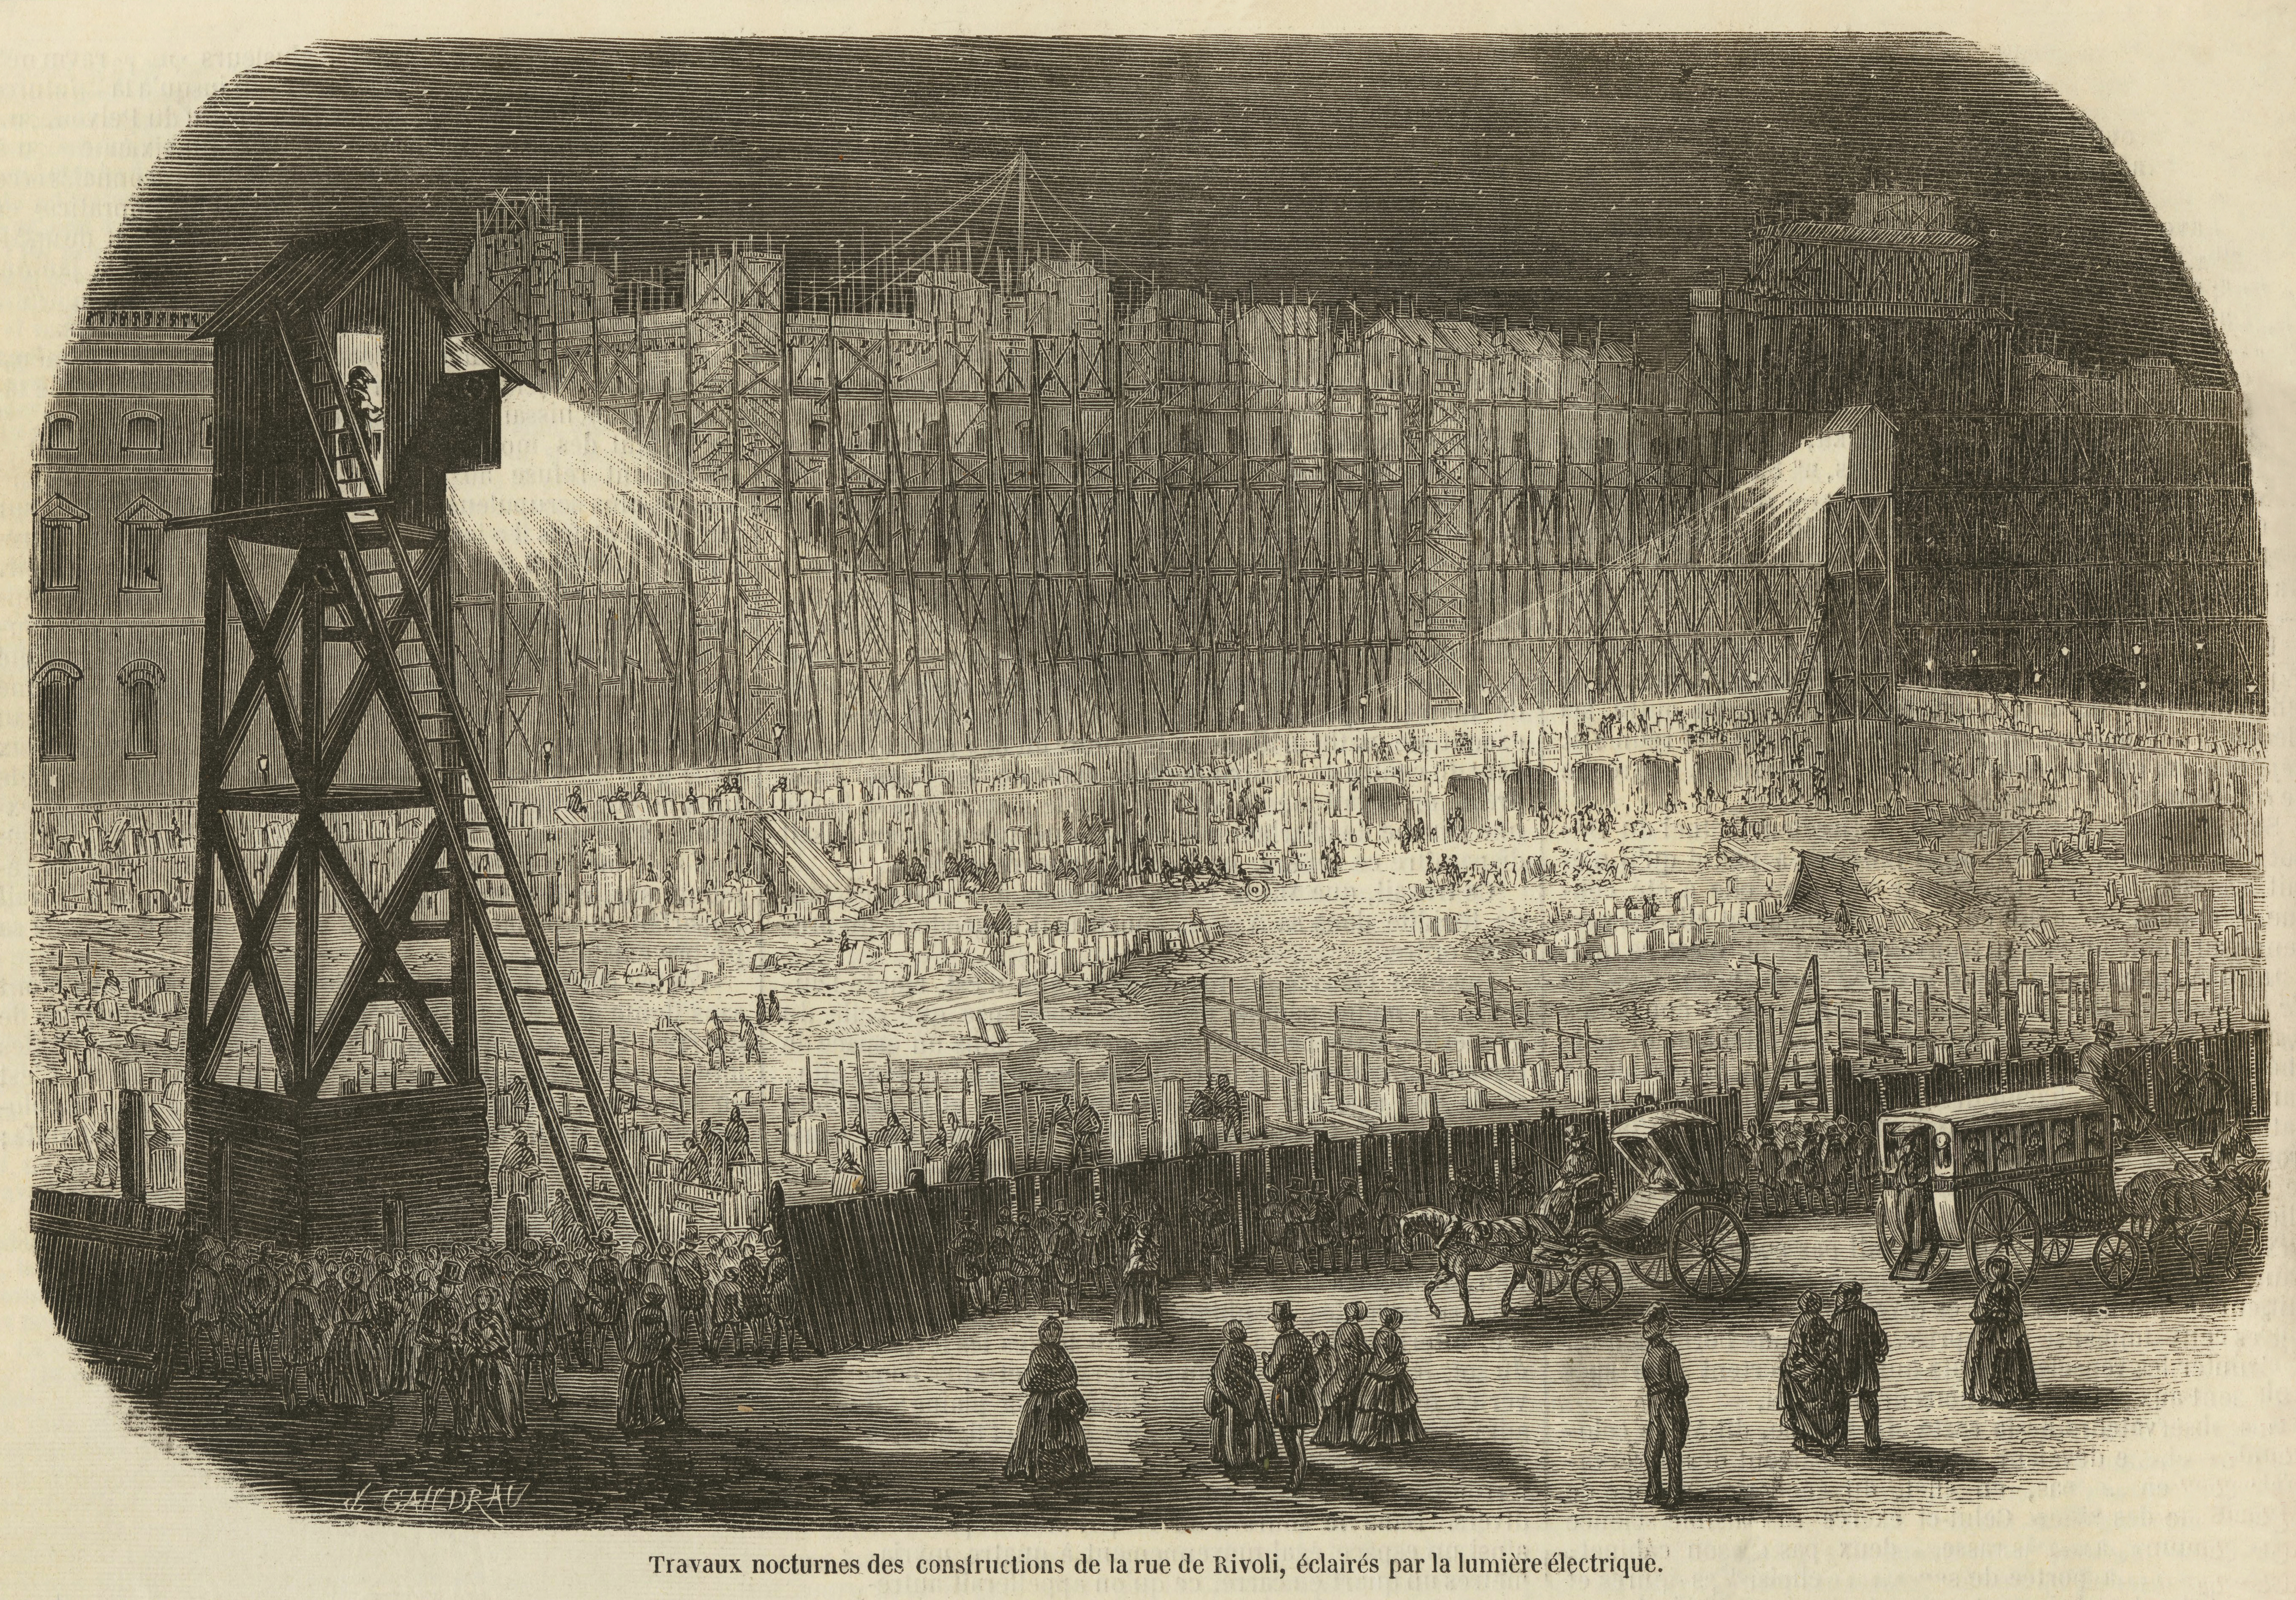
\includegraphics[width=1\textwidth]{2-cap1/complementos/fotos/rivoli.jpg}{\par \footnotesize Construção noturna da \textit{Rue de Rivoli}\textbf{Fonte:} \url{https://commons.wikimedia.org/wiki/File:Travaux_nocturnes_des_constructions_de_la_rue_de_Rivoli,_éclairés_par_la_lumière_électrique.jpg}. }
\label{fig:obrasrivoli}
\end{subfigure}
\end{figure}

A análise de exemplos poderia incluir a construção em Viena (Áustria) da \textit{Ringstrasse} e seus prédios monumentais por ordem do imperador Francisco José I (1857-1913) \cite{abercrombie_vienna_1910,abercrombie_vienna_1911,aman_vienna_1911}; poderia incluir o ``embelezamento'' de Bruxelas (Bélgica) sob a regência do burgomestre \textit{Jules Anspach} e do rei \textit{Leopoldo II} (\textit{le roi bâtisseur}, ``o rei construtor''), em especial o tamponamento e canalização do Sena entre 1859 e 1873 \cite{abercrombie_brussels1_1912,abercrombie_brussels2_1912,abercrombie_brussels3_1913}; poderia avançar pela expansão de Barcelona de acordo com o plano pioneiro de \textit{Ildefonso Cerdà} (1860) \cite{aibarbijker_barcelona_1997,ciervo_cerda_1976,soriaypuig_cerda_1995,wynn_barcelona_1979}; poderia seguir pelo \textit{Risanamento} de Florença (1865-1895), Nápoles (1885-1904) e outras cidades italianas em seguida à \textit{Unificazione} \cite{biocca_naples_1992,parisi_napoli_2001,piccinato_igiene_1989,rossi_napoli_2011}\dots Há um longo fio condutor a ligar o higienismo dos primeiro e segundo terços do século XIX ao ``proto-urbanismo'' do último terço deste mesmo século e ao urbanismo do primeiro terço do seguinte --- se é que há, realmente, alguma solução de continuidade, salvo pela escala e escopo das intervenções propostas nestes dois últimos casos. 

\begin{a3paisagem}
\begin{figure}[!htp]
\caption{Planta de situação da capital e da cidade residencial de Berlim e seus arredores --- plano de desenvolvimento dos arredores de Berlim (1856).}
\centering
\includegraphics[height=0.9\textheight]{2-cap1/complementos/mapas/1856_Bauplanungen.jpg}{\par \footnotesize \textbf{Fonte:} \url{https://commons.wikimedia.org/wiki/File:1856_Bauplanungen.jpg}.}
\label{fig:bauplannungen1856} 
\end{figure}
\end{a3paisagem}

\begin{a3paisagem}
\begin{figure}[!htp]
\caption{Plano para Berlim e arredores até Charlottenburg (1862), desenhado por Ferdinand Boehm.}
\centering
\includegraphics[height=0.9\textheight]{2-cap1/complementos/mapas/Boehm_Berlin_1862.jpg}{\par \footnotesize \textbf{Fonte:} \url{http://nbn-resolving.de/urn:nbn:de:kobv:109-opus-104224}. Os 14 departamentos do \textit{plano Hobrecht} estão rotulados como algarismos romanos. Os assentamentos programados estão indicados por letras maiúsculas e ruas por meio de algarismos arábicos, cada um dentro de um departamento de planejamento.}
\label{fig:berlin1862} 
\end{figure}
\end{a3paisagem}

\begin{a3paisagem}
\begin{figure}[!htp]
\caption{Plano de Giuseppe Poggi para Florença (1865).}
\centering
\includegraphics[height=0.9\textheight]{2-cap1/complementos/mapas/1865-planopoggi-florenca.jpg}{\par \footnotesize \textbf{Fonte:} \url{https://commons.wikimedia.org/wiki/File:Piano_Poggi_(Firenze,_1865)_-_1.JPG}.}
\label{fig:florenca1865} 
\end{figure}
\end{a3paisagem}

\begin{a3paisagem}
\begin{figure}[!htp]
\caption{Plano da cidade de Heilbronn, por Reinhardt Baumeister (1879).}
\centering
\includegraphics[height=0.9\textheight]{2-cap1/complementos/mapas/heilbronn.jpg}{\par \footnotesize \textbf{Fonte:} \url{https://commons.wikimedia.org/wiki/File:Stadtbauplan_Heilbronns_von_1879_auf_der_Grundlage_des_Generalbebauungsplanes_von_Reinhard_Baumeister.jpg}. }
\label{fig:heilbronn1879} 
\end{figure}
\end{a3paisagem}

Para os fins desta pesquisa, entretanto, os dois casos paradigmáticos apresentados já demonstram, sem necessidade de análise detalhada de outros exemplos, que o alvo preferencial das políticas do higienismo no século XIX foram os \textit{centros urbanos ditos ``degradados''} e as \textit{construções insalubres}. Ora, mas \textit{quem morava em tais construções e centros era exatamente quem não tinha condições de pagar para morar em imóveis em condições mais higiênicas}; ``higienizar'', ``embelezar'', fazer ``melhoramentos'' implicou, na maioria dos casos, em \textit{processos maciços de remoção dos trabalhadores e dos mais pobres dos bairros centrais}\footnote{No caso francês, \citeonline[p.~445]{faure_paris_2004} registra que ``dos 102 imóveis construidos nos anos 1860 pela companhia imobiliária dos irmãos Péreire, no atual bulevar Voltaire --- ou seja, num \textit{faubourg} do leste de Paris --- apenas 19\% dos apartamentos, dado o valor dos alugueis, parecem, a rigor, acessíveis a famílias operárias, a menos que se trate de cubículos nos sótãos''. Diz ainda que ``as operações de 1849-1853 tiveram como efeito desalojar 9.081 'trabalhadores' \([\dots]\): 2,1\% partiram para os \textit{banlieues}, e a imensa maioria dos outros se distribuiriam nos \textit{faubourgs}, uma reduzida minoria tendo permanecido nos bairros do centro, esperando, sem dúvida, que a continuação das obras não lhes desse caça'' (\Ibidem[p.~445]{faure_paris_2004}). No caso napolitano, tanto antes quanto depois do \textit{Risanamento} \citeonline{serao1906ventre} denunciou o caráter deletério das condições de vida dos trabalhadores mais pobres. No caso vienense, a \textit{Ringstrasse} acentuou a segregação socioespacial já existente, separando os burgueses da nova e resplandescente avenida, os operários dos subúrbios industriais como \textit{Ottakring} e uma pequena burguesia saudosa da antiga cidade \cite[p.~26]{maderthanermuser_vienna_2003}.}. O longo experimento higienista do século XIX interferiu também sobre a moradia, em especial sobre a moradia dos trabalhadores. A \textit{habitação operária} tornou-se, em paralelo à questão sanitária, pauta importante para os gestores públicos e os encontros internacionais de arquitetos e engenheiros: infiltou-se no Congresso Internacional de Higiene de 1878 em Paris \cite{congres_hygiene_1878}, fato repetido nos congressos internacionais de arquitetos de Londres (1908) e Viena (1910) \cite{QUINTOJR1990}, e mereceu um congresso internacional voltado apenas ao seu debate \cite{fleming_housing_1897}. Em nenhum deles, entretanto, chegou-se a qualquer solução definitiva quanto à questão, restringindo-se tais encontros ao relato das experiências locais em habitação operária e a soluções tópicas\footnote{Veja-se, como exemplo, o voto final da sessão plenária de 7 de agosto do Congresso Internacional de Higiene de 1878: depois de longos relatos e debates sobre a habitação dos operários em Paris, Londres, Bruxelas e outras metrópoles europeias, os presentes concordaram numa única recomendação: reforçar a legislação urbanística existente e transformar em exigência legal a instalação de água nas casas para operários \cite[p.~597]{congres_hygiene_1878}.}.

Tudo indica, até o momento, que os conflitos sociais são elemento essencial da produção, apropriação e uso dos territórios urbanos no período. Mas se há conflito social neste âmbito, seria a estética arquitetônica, ela própria, também produto dos conflitos sociais de seu tempo? Ou estaria imune a tal influência?

\subsubsection{As artes de morar: ecletismo e pré-modernismos, por dentro e por fora}\label{subsec:armor}

Entre os estilos arquitetônicos dezenovistas, o que mais interessa a esta pesquisa, pelo que se pôde encontrar nos documentos consultados, é o \textit{eclético}, do qual serão apresentados alguns exemplos --- retirados da magistral coletânea textbf{L’architecture privée au XIXe siècle, sous Napoléon III}, de César Denis Daly --- na \autoref{fig:hotelprimclas}, na \autoref{fig:hotelsegclas}, na \autoref{fig:villaprimclas}, na \autoref{fig:villasegclas1}, na \autoref{fig:villasegclas2} e na \autoref{fig:villaterclas}\footnote{Ao final da dissertação, nos \autoref{cap:anexos}, será possível encontrar plantas selecionadas de prédios residenciais e comerciais construídos entre 1889 e 1930 no distrito de Brotas, que poderão com proveito ser comparados com estes exemplos.}.

% resumidamente conceituado por um especialista como

% \begin{citacao}
% a cultura arquitetônica própria de uma classe burguesa que dava primazia ao conforto, amava o progresso (especialmente quando melhorava suas condições de vida), amava as novidades, mas rebaixava a produção artística e arquitetônica ao nível da moda e do gosto \cite[p.~13]{patetta_ecletismo_1987}.
% \end{citacao}

% A própria etimologia grega da palavra --- o adjetivo \textgreek{ἐκλεκτικός}, \textit{eklektikos}, ``escolhido entre os melhores'', por sua vez derivado de \textgreek{ἐκλεκτός}, \textit{eklektos}, ``escolhido, seleto'' --- indica uma de suas características principais: a escolha pelo arquiteto ou por seus clientes, na tradição arquitetônica passada, de elementos ora coerentes, ora díspares, que compusessem a obra de acordo com o gosto do freguês ou com a função a ser dada ao imóvel. Justo por isto, há enorme heterogeneidade estilística no campo eclético, sendo bastante difícil encontrar elementos comuns que não as justaposições e os revivalismos. 

% Como movimento artístico, o ecletismo ocorre na arquitetura e na arte do século XIX. As primeiras vanguardas desse movimento datam da terceira década do século XIX com a afirmação de pulsões neo-góticas em áreas francófonas e neo-renascentistas em Florença. Por volta de 1840, na França, em reação à hegemonia do estilo greco-romano, os arquitetos começam a propor a retomada de outros modelos históricos como, por exemplo, o gótico e o românico. O principal teórico do ecletismo arquitetônico é o francês \textit{César Denis Daly} (1811-1893) que o entende como ``o uso livre do passado''. Não se trata de uma atitude de simples copista, mas da habilidade de combinar as características superiores desses estilos em construções que satisfaçam a demandas da época por todo tipo de edificação. Na segunda metade do século XIX, o ecletismo tem forte presença na Europa. O estilo \textit{Segundo Império} ou \textit{Napoleão III} é caracterizado pela realização de importantes edifícios ecléticos, como o Teatro Ópera de Paris, projetado por \textit{Charles Garnier} (1825-1898).

\begin{figure}[!htp]
\centering
\caption{\textit{Hôtel privé} de primeira classe no estilo Segundo Império/Napoleão III.}
\includegraphics[width=1\textwidth]{2-cap1/complementos/fotos/daly01-0.JPEG}{\par \footnotesize \textbf{Fonte:} \textbf{L’architecture privée au XIXe siècle, sous Napoléon III:} nouvelles maisons de paris et des environs, de César Denis \citeonline{daly_architecture1_1864}. \par}
\label{fig:hotelprimclas} 
\end{figure}

\begin{figure}[!htp]
\centering
\caption{\textit{Hôtel privé} de segunda classe no estilo Segundo Império/Napoleão III.} 
\includegraphics[width=1\textwidth]{2-cap1/complementos/fotos/daly01-1.JPEG}{\par \footnotesize \textbf{Fonte:} \textbf{L’architecture privée au XIXe siècle, sous Napoléon III:} nouvelles maisons de paris et des environs, de César Denis \citeonline{daly_architecture3_1864}. \par}
\label{fig:hotelsegclas} 
\end{figure}

\begin{figure}[!htp]
\centering
\caption{\textit{Villa suburbaine} de primeira classe no estilo Segundo Império/Napoleão III.}
\includegraphics[width=1\textwidth]{2-cap1/complementos/fotos/daly03-4.JPEG}{\par \footnotesize \textbf{Fonte:} \textbf{L’architecture privée au XIXe siècle, sous Napoléon III:} nouvelles maisons de paris et des environs, de César Denis \citeonline{daly_architecture3_1864}. \par}
\label{fig:villaprimclas} 
\end{figure}

\begin{figure}[!htp]
\centering
\caption{\textit{Villas suburbaines} de segunda classe no estilo Segundo Império/Napoleão III.}
\begin{subfigure}[b]{0.8\linewidth}
\includegraphics[width=0.9\textwidth]{2-cap1/complementos/fotos/daly03-5.JPEG}
\caption{\textbf{Fonte:} L’architecture privée au XIXe siècle, sous Napoléon III: nouvelles maisons de paris et des environs, de César Denis \citeonline{daly_architecture3_1864}.}
\label{fig:villasegclas1}
\end{subfigure}
\
\begin{subfigure}[b]{0.8\linewidth}
\includegraphics[width=0.9\textwidth]{2-cap1/complementos/fotos/daly03-6.JPEG}
\caption{\textbf{Fonte:} \textbf{L’architecture privée au XIXe siècle, sous Napoléon III:} nouvelles maisons de paris et des environs, de César Denis \citeonline{daly_architecture3_1864}.}
\label{fig:villasegclas2}
\end{subfigure}
\end{figure}

\begin{figure}[!htp]
\centering
\caption{\textit{Villa suburbaine} de terceira classe no estilo Segundo Império/Napoleão III.}
\includegraphics[width=1\textwidth]{2-cap1/complementos/fotos/daly03-8.JPEG}{\par \footnotesize \textbf{Fonte:} \textbf{L’architecture privée au XIXe siècle, sous Napoléon III:} nouvelles maisons de paris et des environs, de César Denis \citeonline{daly_architecture3_1864}. \par}
\label{fig:villaterclas} 
\end{figure}

% As diferentes linguagens artísticas foram reelaboradas a critério do arquiteto seguindo a sua inspiração pessoal. No princípio a tendência eclética se impôs especialmente na realização de estruturas para festas e grandes eventos; sucessivamente, começou a ser apreciada também para mobiliar casas e jardins, nos quais, frequentemente e de forma totalmente acrítica, misturavam-se tempos gregos, vasos árabes e pavilhões indianos. Na época afirmou-se o costume de mobiliar cada sala das residências mais luxuosas segundo um estilo diferente. Assim, marceneiros e ebanistas, por exemplo, tiveram que aprender a lidar com formas bastante diferentes entre si. 

% Mas foi o modernismo industrial do século XIX que serviu como trampolim para o sucesso do estilo eclético. Em 1851, pela primeira vez, na \textit{Great Exhibition} em Londres foram realizados pavilhões onde os mercadores das principais nações do mundo foram chamados para expor suas próprias obras. Percebeu-se que as empresas presentes exibiam para a atenção do publico obras que mostravam a história recente ou antiga da própria nação. Houve euforia em expor todas as obras antigas remodeladas, havendo-se, inicialmente, um certo grau de dependência relativamente aos modelos originais, quase como se fosse uma cópia, uma reprodução. A fantasia de cada artista, artesão, arquiteto, ourives, etc. não demorou para se afirmar, levando os artistas a formular obras personalizadas que ``condensavam'' vários séculos de história. Era isso o que os clientes queriam, curiosos por artes distantes e citações culturais magníficas mostrando que aquela geração iria reviver uma era áurea. Todas as grande técnicas do passado reviviam numa miríade de moveis, cerâmicas e
objetos do Ecletismo.

% Grosso modo, as obras arquitetônicas em estilo eclético podem ser classificadas em três categorias principais, cujas características são assim definidas:

% \begin{itemize}
% \item A \textit{composição estilística}: caracteriza-se por um \textit{maior rigor filológico} e pela \textit{imitação precisa e coerente de um único e preciso estilo arquitetônico}. Os exemplos mais destacados são o \textit{neogrego}, o \textit{neo-egípcio} e o \textit{neogótico}.
% \item O \textit{historicismo tipológico}: caracteriza-se por uma \textit{relação apriorística de cunho analógico entre estilo e função} através de valores associativos, não raro arbitrários. A arquitetura medieval, por exemplo, forneceu aos arquitetos os traços místicos e a religiosidade para as novas igrejas; na arquitetura renascentista foram encontradas as características áulicas elegantes para os edifícios públicos; na arquitetura barroca, ou nos estilos orientais, a festividade exigida pelos equipamentos; no classicismo pesado do coríntio romano, o caráter apropriado aos solenes edificios parlamentares, aos museus e aos ministérios.
% \item Os \textit{pastiches compositivos}: caracterizam-se pela \textit{fusão de elementos arquitetônicos de estilos distintos, historicamente inadmissíveis}, sob cujos elementos díspares, não raro beirando o mau gosto, mascaravam-se muitas vezes soluções estruturais inovadoras \cite[p.~14-15]{patetta_ecletismo_1987}.
% \end{itemize}

A literatura especializada por muito tempo divergiu acerca do eclético. Primeiro considerou-o como o estilo ostentatório dos \textit{nouveaux riches} desprovidos da bagagem cultural do \textit{Ancièn Régime} e dispostos a demarcar seu espaço social por meio da sobreposição, às vezes sem nexo, das novas modas da Escola de Belas-Artes de Paris \cite[pp.~315-319]{guerrand_espacos_2009}. Num momento seguinte, considerou-o um estilo arquitetônico com méritos e conquistas próprios, em processo de redescoberta desde pelo menos a metade dos anos 1970, a partir da crítica ao ideário arquitetônico do Modernismo que o sucedeu e criticou duramente \cite{almeida_victoria_1997, almeida_vitrinescomercio_2014, patetta_ecletismo_1987, puppi_hisnamod_1998}. A discussão sobre a \textit{natureza estética} do eclético, ou de seus \textit{méritos técnicos e arquitetônicos}, é totalmente marginal a esta pesquisa. Interessa, sim, o fato de o eclético ser o estilo arquitetônico mais encontrado no distrito soteropolitano estudado.

%, especialmente nas modalidades de \textit{historicismo tipológico} e \textit{pastiche compositivo}, com maior frequência esta última.

A América Latina foi terreno fértil para as experimentações arquitetônicas, especialmente as ecléticas, e isto por questões muito particulares. No final do século XIX, findos os processos independentistas, consolidadas as fronteiras nacionais e assentados os blocos hegemônicos na política após um século pontilhado por guerras, \textit{pronunciamientos} e rebeliões, as classes dominantes nos países latinoamericanos viram na arquitetura um meio de reafirmar sua identidade nacional. Curiosa e paradoxalmente, entretanto, tal como em outros campos da cultura, esta reafirmação se deu por meio de símbolos e elementos tomados de empréstimo por estas mesmas classes dominantes às edificações da aristocracia, dos banqueiros, dos grandes comerciantes e industriais da Europa \cite[pp.~403-406]{gutierrez_arquibero_1983}. Conquanto haja leitura destes empréstimos no sentido de criar uma clivagem entre colonizados e colonizadores, em que os primeiros --- como um todo, sem qualquer clivagem, estruturação, estratificação ou hierarquização social internas a si próprios --- encontrar-se-iam sempre no encalço destes últimos por quaisquer razões \cite{bhabha_local_1998,memmi_coloniza_1967}, na perspectiva adotada por esta pesquisa parece mais plausível radicar estes empréstimos nos deslocamentos miméticos de ideias e práticas devido à \textit{inserção subordinada destas classes dominantes no capitalismo internacional e no colonialismo} \cite{schwarz_ideias_1973}. As duas correntes, entretanto, concordam em que o deslocamento de ideias, símbolos e signos de seu contexto original produz efeitos bastante diversos no novo contexto em que se inserem, e que são eles, e não aqueles produzidos em seu ambiente de origem, que devem ser estudados. Esta ``chave de leitura'' será importante para a análise da urbanização brasileira na Primeira República, mais adiante.

E aqui, nesta etapa ``pré-modernista'' do pensamento e da prática acerca das cidades, se encerram as condicionantes sincrônicas internacionais relevantes para a presente pesquisa. As defasagens entre a produção e circulação de ideias nos meios profissonaics levam a que as primeiras influências da arquitetura e do urbanismo europeus de vanguarda surgidas entre a última década do século XIX e as duas primeiras décadas do século XX, em seu pensamento ou realizações, só se façam sentir sobre o pensamento e a prática da arquitetura e do urbanismo em Salvador nos trabalhos da Semana de Urbanismo de 1935, que extrapolam o limite temporal escolhido\footnote{É certo, por exemplo, que Theodoro Sampaio mencionou explicitamente a influência sobre ele exercida pelas cidades-jardim \cite{costa1996theodoro}, e que já em 1913 estas mesmas cidades-jardins eram debatidas na imprensa baiana como contraponto ao desleixo da administração pública com o problema das moradias populares \cite{flexor_salvadorverde_2000}; apesar disto, nem o projeto da Cidade da Luz foi adiante (sua implementação em 1937 se deu vinte e oito anos depois da apresentação do projeto original de Theodoro Sampaio), nem os debates na imprensa avançaram além do confronto de ideias.}.
\section{A inserção brasileira no contexto internacional}\label{sec:insbrascontint}

É tempo, agora, de entender a inserção brasileira num contexto internacional de imperialismo, guerras, trustes e carteis. Nesta escala, já é possível analisar mais cerradamente a formação social e analisar, ainda que superficialmente, sua estrutura de classes, para, posteriormente, verificar a inserção da sociedade soteropolitana neste quadro.

\subsection{Da República da Espada (1889-1894) à República do Café-com-Leite (1894-1930)}\label{subsec:espadaleite}

A proclamação da república no Brasil (1889) resulta não apenas das questões \textit{religiosa}\footnote{Costuma-se dar este nome a uma série de conflitos ocorridos entre 1873 e 1876 entre o clero e a maçonaria, de um lado, e entre o clero e a instituição regalista do \textit{padroado}, de outro; ambos podem ser enquadrados na \textit{reação ultramontana católica} iniciada no papado de Gregório XVI (1831-1846) e continuada no papado de Pio IX (1846-1878), especialmente por meio da encílica \textit{Quanta Cura} e seu infame anexo \textit{Sílabo dos Erros} (1864) e das posturas mais duras do Concílio Vaticano I (1869-1870), como resposta às revoluções liberais e ao secularismo. O conflito do clero com a maçonaria já se antecipava enquanto ordem papal em \textit{Quanta Cura} e no \textit{Sílabo dos Erros}, ambos contrários à liberdade de consciência e ao primado da razão; restou que Vital de Oliveira, bispo de Olinda, e Macedo Costa, bispo do Pará, acendessem o pavio aplicando tais doutrinas a seu pastorado, proibindo maçons em irmandades católicas, punindo padres maçons e engajando-se em polêmica impressa contra a maçonaria. O caso chegou até à Coroa, pois o regalismo instituído pelo padroado facultava ao imperador brasileiro interferir em assuntos clericais -- na prática, a igreja era quase totalmente submissa à Coroa, fato condenado tanto em \textit{Quanta Cura} quanto no \textit{Sílabo dos Erros}. Com a subsequente prisão dos bispos por desobedecerem à ordem imperial de suspender as sanções religiosas que haviam imposto aos maçons, a questão tomou vulto, transformou-se em transtorno diplomático com o Vaticano, resolvido com a absolvição imperial dos bispos em 1876, passando assim a Pedro II a imagem de ``submisso ao Papa'' tão fortemente aproveitada pela campanha republicana então nascente.}, \textit{militar}\footnote{Entre 1884 e 1887, uma série de incidentes envolvendo o tenente-coronel Antonio de Sena Madureira e o coronel Ernesto Augusto da Cunha Matos em questões que iam desde protestos quanto à contribuição obrigatória para o montepio militar ou o afastamento de oficiais acusados de corrupção geraram intensa polêmica impressa, resultando na proibição, por parte do Ministério da Guerra, de qualquer manifestação de militares através da imprensa. A mordaça gerou insatisfação na caserna, especialmente na Escola Militar da Praia Vermelha, onde já floresciam a filosofia positivista e o republicanismo.} ou mesmo da questão \textit{sucessória}\footnote{Uma vez que Pedro II teve apenas filhas como herdeiras e a constituição brasileira de 1824 instituíra a sucessão semi-agnática, que não exclui herdeiras do processo sucessório, Isabel era a herdeira do trono brasileiro; por ser casada com Luís Filipe Maria Fernando Gastão, conde d'Eu, tido como largamente impopular em razão de sua nacionalidade francesa, sua futura ascensão ao trono criou entre as classes populares, a classe média, os militares e outros a má expectativa de serem governados por um estrangeiro.}; por importantes que sejam estas questões como expressão das contradições e conflitos sociais do último período do Império, foi fundamentalmente da crise aberta pela \index{abolição da escravidão}\textit{abolição da escravidão}, como corolário da degenerescência do regime escravista, que resultaram os problemas sociais e políticos que levaram à derrocada do Império. 

Foi, na verdade, nos anos 1860 que se acumularam fatores contrários à sustentação do regime escravista: a crise econômica dos anos 1860, causada pelo declínio nos preços do café (principal pauta de exportação brasileira na época); a crise financeira de 1864; a vitória dos Estados antiescravistas na Guerra de Secessão estadunidense, com o consequente debilitamento dos Estados escravocratas (Brasil e Cuba) perante a opinião pública internacional; a Guerra do Paraguai, onde massas de recém-libertos incorporadas à tropa são tomadas pelas ideias de liberdade e insuflaram-nas entre a oficialidade; o declínio da população escrava e as migrações internas de escravos, especialmente do Norte-Nordeste, para as regiões cafeeiras; tudo isto, enfim, resultou não apenas numa cúpula ministerial favorável à abolição, mas também ao florescimento de uma opinião pública também abolicionista, e ao surgimento das primeiras associações dedicadas à propaganda anti-escravista e à coleta de donativos para compra de alforrias \cite[p.~141-143]{gorender_escrareab_1990}.

É igualmente o momento em que não apenas a rebelião negra contra a escravidão, afogada pela maré montante da repressão no início do período, assume ao seu final novas formas e se intensifica; é de igual modo momento do dealbar, na cena política e social, de uma classe média urbana patrocinadora de um movimento abolicionista radicalizado, promotor não só da cotização para alforrias, mas igualmente de fugas individuais e coletivas de escravos \cite[p.~267-336]{saes_estadoburgues_1985}.

A \textit{abolição da escravidão} (1888) e a \textit{proclamação da república} (1889) fazem parte de um só processo de conflitos sociais no Império, em que as oligarquias agrárias enfrentaram não apenas os escravos rebeldes, mas igualmente uma classe média urbana estreante no cenário político; entendê-las separadamente implica numa separação injustificada entre entre uma esfera econômica e uma esfera política que só se podem compreender juntas. E muitas das contradições e conflitos sociais da Primeira República foram ensaiados já neste processo.

\subsubsection{A curta República da Espada (1889-1894)}\label{subsubsec:espada}

O período imediatamente posterior à proclamação da república no Brasil foi convulsionado por agitações políticas de todos os tipos. Em disputa, não somente projetos políticos, mas o poder, e, em última instância, mesmo o regime.

A crônica da época diz que o golpe militar responsável pela proclamação da república foi articulado por um grupo de jovens oficiais sem muita inserção entre a base da tropa e sem maior articulação com o oficialato superior, convocado à última hora para a ação \cite[p.~16]{cardoso_govmil_1977}; por frágil que fosse, esta articulação abriu um período de rearticulação das bases e das forças sociais hegemônicas do país. 

Durante a ditadura militar conhecida como \textit{República da Espada} DESENVOLVER RELACIONANDO CONTRADIÇÃO ENTRE CAFEICULTORES E MILITARES

O governo de Floriano Peixoto foi uma nota dissonante. Ele pensava em construir um governo estável, acima das disputas locais, estaduais e regionais, cooptando quadros nas escolas civis e militares. Teria tudo para ser ferrenho adversário dos oligarcas agrários, mas rapidamente surgiu uma aliança entre Floriano e o Partido Republicano Progressista (PRP), pois ambas as partes percebiam os riscos que corria a jovem república e viam-se como garantidores do novo regime: os oligarcas, por perceberem em Floriano a única possibilidade de garantir a sobrevivência do regime contra as forças centrífugas já então em pleno curso\footnote{EXPLICAR}; DESENVOLVER FAZENDO A PASSAGEM PARA CAMPOS SALES

Em defesa da república, surgem durante o governo Floriano Peixoto os ``jacobinos'' de 1893-1897, agrupados em torno de jornais como \textit{O Jacobino} e \textit{O Nacional}: gente como Júlio de Castilhos, Francisco Glicério, Deocleciano Martyr, Aníbal Mascarenhas e outros. Agitadores políticos profissionais, autoritários, anticlericais, defensores de medidas nacionalistas (tarifas de proteção à indústria e nacionalização do solo) e protetivas dos trabalhadores (como a jornada de oito horas e a regulamentação dos alugueis para operários), americanófilos e antilusitanos, atuavam ameaçando de morte os inimigos, intimidando-os com a publicação de seus nomes na sua imprensa (de longe a mais radical do período), provocando confrontos de rua, agitando o povo para depredações, insuflando ataques a portugueses (que tratavam, sem mais, como monarquistas) etc. \cite{queiroz_radicais_1986}\dots Tinham como base social principal o pequeno funcionalismo público e os militares de baixa e média patente. Com a perseguição aos suspeitos de envolvimento no atentado contra o presidente Prudente de Morais (5 nov. 1897), o movimento perdeu força e dissolveu-se.

Movimento monarquista (até declínio em 1910) \cite{CARONE1970inst,janotti_subversivos_1986} DESENVOLVER COMO A BAHIA FOI FOCO DO MOVIMENTO MONARQUISTA NO COMEÇO DA REPÚBLICA

\subsubsection{A longa República do Café-com-Leite, ou a Política dos Governadores (1894-1930)}\label{subsubsec:cafeleite}

DESENVOLVER EM SÍNTESE APERTADA, USANDO A Periodização de Edgar Carone: apogeu (Prudente de Moraes, Campos Sales, Rodrigues Alves, Afonso Pena), abalos (Hermes da Fonseca, Wenceslau Braz), contestações (Epitácio Pessoa, Artur Bernardes, Washington Luiz) \cite{carone_evolucao_1977}

DESENVOVER, EM SÍNTESE APERTADA A POLÍTICA DOS GOVERNADORES - funcionamento, altos e baixos 

DESENVOLVER O ARGUMENTO DE PERISSINOTO, NELSON WERNECK SODRÉ E BORIS FAUSTO; CONFLITOS REGIONAIS COMO CONFLITO ENTRE DIFERENTES FRAÇÕES REGIONAIS DOS LATIFUNDIÁRIOS, DIVIDIDOS ENTRE EXPORTADORES E PRODUTORES PARA O MERCADO INTERNO

\subsection{O Brasil, a banca internacional, o imperialismo}\label{subsec:brasimper}

A abolição e a proclamação da República criaram o quadro institucional adequado para a crescente integração do Brasil na economia capitalista mundial e colocaram o Brasil em posição de maior destaque na divisão internacional do trabalho, com um crescimento de 31,6\% nas exportações brasileiras entre 1880 e 1900 e de 63,7\% na primeira década do século XX \cite[p.~352]{singer_braecomu_1977}. 

Esta maior inserção, entretanto, se deu ainda no papel de fornecedor de matérias-primas e de produtos agrícolas, especialmente café (o principal produto da pauta de exportação brasileira), açúcar, algodão, borracha e derivados do couro.

\begin{table}[!htp]
\IBGEtab{
\caption{Brasil, principais produtos de exportação, 1889-1929 (em \%)}\label{tab:exportabrasil}}
{
\begin{minipage}{21cm}
\begin{tabular}{cccccccccc}
\hline
Períodos & Café & Açúcar & Cacau & Mate & Fumo & Algodão & Borracha & Couros/Peles & Outros \\
\hline\hline
1889-1897 & 67,8 & 6,5 & 1,1 & 1,2 & 1,7 & 2,9 & 11,8 & 2,4 & 4,8 \\
1898-1910 & 52,7 & 1,9 & 2,7 & 2,7 & 2,8 & 2,1 & 25,7 & 4,2 & 5,2 \\
1911-1913 & 61,7 & 0,3 & 2,3 & 3,1 & 1,9 & 2,1 & 20,0 & 4,2 & 4,4 \\
1914-1918 & 47,4 & 3,9 & 4,2 & 3,4 & 2,8 & 1,4 & 12,0 & 7,5 & 17,4 \\
1919-1923 & 58,8 & 4,7 & 3,3 & 2,4 & 2,6 & 3,4 & 3,0 & 5,3 & 16,5 \\
1924-1929 & 72,5 & 0,4 & 3,3 & 2,9 & 2,0 & 1,9 & 2,8 & 4,5 & 9,7 \\
\hline
\end{tabular} 
\end{minipage}
}
{ \fonte{Elaboração do autor, com dados de \citeonline[p.~63]{suzigan_polgov_2001}.} }
\end{table}

\begin{table}[!htp]
\centering
\IBGEtab{
\caption{Principais parceiros do Brasil no comércio internacional 1853-1928}\label{tab:comerbras}}
{\begin{tabular}{ccccccccc}
\hline
\multicolumn{9}{c}{Participação em \% no comércio exterior do Brasil} \\
\hline & \multicolumn{2}{c}{Grã-Bretanha} & \multicolumn{2}{c}{Alemanha} & \multicolumn{2}{c}{Estados Unidos} & \multicolumn{2}{c}{França} \\
\cline{2-9} Datas & Exp. & Imp. & Exp. & Imp. & Exp. & Imp. & Exp. & Imp. \\
\hline\hline
1853/4 a 1857/8 & 32,9 & 54,8 & 6,0 & 5,9 & 28,1 & 7,0 & 7,8 & 12,7 \\
1870/1 a 1872/4 & 39,4 & 53,4 & 5,9 & 6,5 & 28,8 & 5,4 & 7,5 & 12,2 \\
1902 a 1904 & 18,0 & 28,1 & 15,0 & 12,2 & 43,0 & 11,5 & 7,8 & 8,8 \\
1908 a 1912 & 17,0 & 27,5 & 14,3 & 16,2 & 38,2 & 13,5 & 8,6 & 9,4 \\
1920 & 8,2 & 21,4 & 5,8 & 4,6 & 42,0 & 40,6 & 12,0 & 5,4 \\
1928 & 3,4 & 21,0 & 11,0 & 12,3 & 44,6 & 26,2 & 9,0 & 6,2 \\
\hline
\end{tabular} }
{ \fonte{\citeonline[p.~369]{singer_braecomu_1977}} }
\end{table}

Para piorar, a fase monopolista do capitalismo, já detalhada na \autoref{sec:1.2}, implicava em enorme integração vertical e horizontal dos conglomerados empresariais, e igualmente de preferência pelos produtos destes conglomerados nas ``zonas de influência'' de seus países de origem; por isto, à exceção do café, para cuja produção o Brasil tinha características ecológicas excelentes, todos os demais produtos da pauta de exportação encontravam ou a concorrência de similares produzidos nas áreas de atuação dos conglomerados imperialistas (p. ex., açúcar de beterraba), ou o obstáculo de taxas aduaneiras protecionistas.

Percival Farquhar, conhecidíssimo capitalista estadunidense atuante no Brasil durante a República Velha \cite{CUNHA2011}, praticamente delineou, num artigo publicado em meio à guerra, o programa da ação dos investidores estrangeiros no país:

\begin{citacao}
Os notáveis investimentos na América do Sul serão, naturalmente, em estradas de ferro; serviços públicos urbanos; desenvolvimento da energia hidrelétrica; propriedades cujos produtos sejam consumidos nos Estados Unidos; títulos da dívida do governo federal, dos governos estaduais e dos municípios. \cite[p.~398]{farquhar_invest_1916}
\end{citacao}

Com algumas variações, este foi, na verdade o programa de atuação de todos os investidores estrangeiros no Brasil durante a Primeira República -- e o próprio Farquhar, por agir nas bancas de Londres, Paris e Bruxelas em busca de capital para seus empreendimentos, pode ser tomado como personagem-síntese desta atuação.

No que diz respeito aos empréstimos tomados pelo país junto à banca internacional, se apenas dois dos dos 17 empréstimos tomados pelo Brasil durante o Império se destinaram a investimentos em infraestrutura (estradas), após 1890 passam a se destinar majoritariamente a obras públicas (construção de portos e ferrovias) ou à sustentação das cotações externas de café. As dificuldades na quitação destas dívidas, comuns no Império, persistiram nas primeiras décadas da República: os dois \textit{funding loans} (1898 e 1914) foram pactuados pelo governo federal com a banca internacional mediante a cessão a exigências draconianas por esta última \cite[p.~365]{singer_braecomu_1977}.

\subsubsection{O capital britânico}\label{subsubsec:capbrit}

Os britânicos foram os principais beneficiados pela abertura dos portos brasileiros em 1808, e desde então dominaram o comércio externo e a banca brasileira.

A contração gradual começou por volta de 1928-1929 com a venda de diversos serviços públicos para corporações controladas por capitalistas estadunidenses, iniciando uma tendência sem retorno \cite{rippy_britlat_1954}.

DSENVOLVER USANDO A TABELA DE RIPPY

\subsubsection{O capital francês}\label{subsubsec:capfran}

Se os empresários franceses se faziam presentes no Brasil desde há muito, foi só durante a Primeira República brasileira que os investimentos franceses floresceram, como parte de uma tendência geral para investimento francês na América Latina (concentrado no Brasil, Argentina e México). Entre 1902 e 1914, os investimentos franceses na América Latina duplicaram, e os investimentos no Brasil passaram de 20\% a 42\% do total; além disso, em 1913 os investimentos diretos (ou seja, em empresas) ultrapassaram os empréstimos públicos, que até 1902 sempre haviam sido muito maiores em comparação \cite[p~83-84]{mauro_empfran_1999}. Entre 1904 e 1913 o Brasil foi o maior cliente da banca francesa na região, e o segundo em escala mundial \cite{rippy_french_1949}. 

Havia três destinos principais para os investimentos franceses: \textit{(a)} os \textit{portos}, em especial os de Recife, Porto Alegre e Rio de Janeiro; \textit{(b)} as \textit{ferrovias}, com especial destaque para a criação de seis companhias francesas específicas no setor e da  (1910), com capital de 3 milhões de francos, para a construção de ferrovias na Bahia; \textit{(c)} os \textit{bancos} \cite[p~84]{mauro_empfran_1999}, que merecem destaque.

O \textit{Banque Française au Brésil}, fundado em 1872 com capital de 10 milhões de francos, tornou-se lucrativo a partir de 1880, e mais ainda depois de 1900; o sistema financeiro francês, entretanto, ainda era insuficiente, o que levou à criação em 1909 do \textit{Banque Française et Italienne por l'Amérique du Sud} (conhecido posteriormente como \textit{Banco Sudameris}) \cite[p~84]{mauro_empfran_1999}. Entre um e outro, foram criados também o \textit{Banque Nationale du Brésil} (1893) e o \textit{Crédit Foncier du Brésil et de l'Amérique du Sud} (1907), este último tendo especial relevo nas muitas reformas urbanas realizadas no Brasil da Primeira República.

Os investimentos franceses no período gozaram de alta rentabilidade (taxas anuais de 5\%, com retorno rápido e prazos de amortização superiores a 35 anos), mas após a Primeira Guerra Mundial o franco se desvalorizou frente à libra esterlina, levando a uma conflituosa redução da dívida que só foi resolvida quando a Corte Internacional de Haia obrigou os devedores brasileiros a indexar a dívida segundo o franco-ouro \cite[p.~87]{mauro_empfran_1999}. Mesmo assim, em 1922 já havia 4 bilhões de francos investidos no Brasil\footnote{Distribuídos da seguinte maneira: 2,5 bi para empréstimos públicos, 1,25 bilhão para ferrovias, 170 milhões para bancos e 138 milhões para a indústria \cite[p~84]{mauro_empfran_1999}.}.

Até 1930, Pierre Louis Marcel Boilloux-Lafont era o mais importante capitalista francês a se relacionar com investidores e com o Estado brasileiro. Dono da \textit{Caisse Commerciale et Industriale} (fund. 1907), banco especializado em empréstimos estrangeiros, veio ao Brasil em 1909 para assumir a construção do porto de Salvador, e em 1911 conseguiu decreto autorizador do funcionamento da sua \textit{Societé Franco-Sud-américaine de Travaux Publics} no ramo da construção de estradas de ferro no Brasil; os 326 milhões de francos do grupo Boilloux-Lafont investidos no Brasil em 1914 representavam 10\% do total do investimento francês no país \cite{somogyi_lafont_1990}.

FALAR TAMBEM DO BARÃO FRANCÊS MUITO CITADO POR JOACI CUNHA

\subsubsection{O capital alemão}\label{subsubsec:capale}

As estatísticas divergem em alguns aspectos, mas é certo que a migração alemã para a América Latina não tomou vulto antes da década de 1850 \cite[p.~65]{rippy_german_1948} e só se tornou realmente significativa entre os anos 1880 e 1910 (cf. \autoref{tab:imigra}). Os primeiros migrantes foram responsáveis pelos primeiros empreendimentos comerciais de países latino-americanos com a Alemanha (antes mesmo da unificação) e por atrair investimentos alemães em terras, pecuária, imóveis, suprimentos agrícolas, cervejarias, hoteis e estabelecimentos mercantis. 

Havia na América Latina inteira em 1918 pelo menos 1.019 empresas com capital alemão, mobilizando US\$ 677 milhões \cite[p.~64-65]{rippy_german_1948}\footnote{As cifras estão em dólares, unusualmente para as estimativas do período, porque retiradas de \textit{blacklists} estadunidenses de empresas com participação alemã, usadas pelo governo dos EUA durante a Primeira Guerra Mundial como instrumento político para convencer governos latino-americanos a expulsar de seus respectivos países, ou ao menos de romper negócios e contratos pré-existentes.}. Ainda antes da Primeira Guerra Mundial, havia um pequeno circuito bancário alemão -- pequeno quando comparado com os circuitos britânico e francês -- constituído na América Latina: \textit{Banco Aleman Transatlantico}, \textit{Banco Germanico de la América del Sud}, \textit{Brasilianische Bank für Deutschland}, \textit{Banco de Chile y Alemania}, \textit{Banco Antioqueña}, \textit{Banco Mexicano de Comercio e Industria} e \textit{ZentralAmerika Bank}. Havia também outra especialidade alemã na América Latina, as empresas de navegação: Hamburg-American, Hamburg-South American, North German Lloyd, Hansa, Kosmos, Roland, Atlas e Kirsten Line \cite{rippy_german_1948}.

Não obstante sua presença marcante no campo da eletricidade e da química, reais especialidades da indústria alemã no período, em outros aspectos o capital alemão na América Latina era insignificante frente aos capitais britânico e francês. Antes da Primeira Guerra Mundial o capital alemão tinha pouca participação no setor de serviços públicos, somente duas petrolíferas, menos de doze mineradoras, quatro companhias de nitratos e três ferrovias (no valor total de US\$ 25 milhões), e participação tímida na indústia de processamento de carne, na navegação fluvial e na telefonia \cite{rippy_german_1948}. No Brasil, entretanto, sua presença foi marcante no setor agrícola.

MENCIONAR OS WILDBERGER COMO PARTE DO COMPLEXO GERMÂNICO; JUSTIFICAR A INCLUSÃO DE SUÍÇOS NESTA CATEGORIA

\subsubsection{Quadro geral}\label{subsubsec:quager}

ESCREVER TRANSIÇÃO AO CAPÍTULO

O Brasil já estava em recessão em 1928 \cite{hautcoeur_1929_2009} DESENVOLVER COM BASE NOS ARGUMENTOS DO AUTOR; POSIÇÃO POLÊMICA

A Bolsa do Café de Santos, um belíssimo prédio onde eram feitos pregões, registrava a tragédia em cifras: em agosto de 1929, dois meses antes da implosão da bolsa nova-iorquina, a saca do café estava cotada no mercado internacional em 200 mil-réis, em janeiro de 1930 desabara para 21 mil-réis. A praça de Santos, o maior centro brasileiro de atividades comerciais ficou virtualmente em moratória. Sem preços, o Brasil, que possuía 60\% do mercado internacional do café, não podia exportar o produto, e acumulava grandes estoques nos diversos armazéns gerais da cidade -- o que comprometeu os preços \cite{hautcoeur_1929_2009}.

CONTINUAR

\subsection{Classes sociais e política na Primeira República}\label{subsec:clapolprire}

Seria muito simples pegar a estrutura econômica brasileira e fazer derivar uma categoria profissional de cada um dos lugares na produção e, posteriormente, agrupá-los em classes mediante o critério da posse, propriedade ou controle dos meios de produção. 

Mas é isto suficiente?

Há vasta literatura recomendando prudência nesta caracterização \cite{aguiar_hierarquias_1974, BERNARDO1991, bernardo_fascismo_2015, ossowski_classes_1964, schumpeter_imperialismo_1961, velho_classes_1977}. Não há uma só entre as referências metodológicas consultadas que recomende tal simplismo empirista. É preciso, sim, entender como as classes se relacionam com seu lugar na produção econômica; entretanto, sem a força viva dos embates cotidianos e das pequenas coisas extra-laborais que fazem qualquer classe social fazer-se enquanto classe ao confrontar-se com outras (costumes, formas de sociabilidade, lazeres, produção cultural etc.), a análise terminaria manca.

Há ainda outra questão. É comum falar-se em ``elites'' para denominar qualquer estrato social dominante em determinado tempo e lugar. Tal classificação não será empregue nesta pesquisa, primeiro por ser vaga e imprecisa; segundo, por não respeitar a longa -- e controversa -- produção sociológica acerca do assunto \cite{bottomore_elites_1965,michels_partidos_1982,mosca_elementi_1923,pareto_mind_1935,
schumpeter_capitalismo_1961} terceiro, por só fazer sentido quando inserida num contexto teórico onde as classes sociais fornecem o substrato básico e as elites, um modo de compreensão da mobilidade social entre diferentes classes. Uma longa citação ajudará a situar o problema:

\begin{citacao}
\dots a referência a uma classe social só adquire sentido através da referência a uma classe oposta. A dialéctica da exploração e da opressão liga intimamente as características e a estrutura interna das várias classes, e sob este ponto de vista a luta entre as classes consiste na transformação conjunta e contraditória de todas elas. Mas não se passa o mesmo com a noção de elite, que pode ser definida de maneira independente, enquanto estrato privilegiado. A estrutura interna de uma elite nem se relaciona com a das massas, pois os teóricos das elites definem a massa precisamente pela sua incapacidade de organização própria, nem está em relação necessária com a estrutura interna de qualquer outra elite, porque a elite governa sozinha e se aparece uma nova é para liquidá-la e substituí-la. [\dots] a teoria das elites é incapaz de explicar, ou sequer conceber, esta transformação dos membros de uma elite em membros de uma classe. Os autores que pretendem que o fenómeno da mobilidade social invalida, ou pelo menos compromete, a teoria das classes e justifica a aplicação de uma perspectiva de elites estão a confundir classe com casta. É precisamente a mobilidade social que permite inserir o fenómeno das elites no quadro geral das classes, pois a formação de uma elite no interior de uma classe inferior prepara a projecção desta elite para a classe superior, alimentada periodicamente por estas novas elites [\dots]. As elites só têm sentido porque são elites de uma classe ou elites de uma classe transformando-se em componentes de outra classe. O conceito de elite padece, portanto, de uma assimetria, porque as elites capitalistas continuam a ser capitalistas, enquanto as elites proletárias abandonam a sua classe de origem. [\dots] a questão decisiva é que não ocorre nenhuma conversão de uma elite numa classe. Ou as elites se formam no interior de uma dada classe exploradora ou os membros da elite da classe explorada se convertem em membros de uma classe exploradora. \cite[p.~387-388]{bernardo_fascismo_2015}.
\end{citacao}

São igualmente inaplicáveis, para os fins desta pesquisa, os conceitos clássicos de \textit{oligarquia} e \textit{aristocracia}. Este último, porque com a proclamação da república foram extintos os títulos nobiliárquicos e todos os cargos políticos foram tornados eletivos pela Constituição de 1891; o primeiro, porque diz respeito a uma \textit{forma de governo} em que o exercício do poder político está restrito a um pequeno número de pessoas, não a uma \textit{classe social}, ou seja, aos fundamentos sociais do próprio poder político.

\subsubsection{Os latifundiários}\label{subsubsec:clagraris}

Dado o fato de a economia brasileira manter sua característica agroexportadora herdada do Império, são os \textit{latifundiários}, sem sombra de dúvida, uma das classes participantes do bloco político hegemônico durante a República Velha \cite{gorender_burguesia_1990,oliveira_emopro_1977,CARONE1970inst}. Há um debate em aberto acerca da natureza sociológica desta classe, em especial no período de transição do Império à República, girando em torno de ter-se ou não transformado numa \textit{burguesia agrária} por força da mudança de padrão da exploração do trabalho (da escravidão ao assalariamento) \cite{gorender_burguesia_1990,oliveira_emopro_1977}; para evitar as polêmicas, serão aqui chamados apenas de \textit{latifundiários} pelo fato de a raiz de seu poder político encontrar-se na exploração da produção agrícola em regime de \textit{plantagem}\footnote{Foi adotada aqui a denominação proposta por Jacob Gorender para o que tradicionalmente se chama \textit{plantation}. Eis a explicação, pelo próprio: ``As grandes explorações agrícolas com trabalho escravo, surgidas no continente americano à época do mercantilismo, têm sido designadas, na literatura de língua portuguesa, pelo nome de \textit{plantation}, vocábulo emprestado ao inglês e sempre impresso em itálico Mas os ingleses [\dots] tomaram o termo emprestado ao francês. [\dots] O esdrúxulo consiste em qu escritores de língua portuguesa precisem desse vocábulo estrangeiro a fim de indicar uma forma de organização econômica que Portugal teve muito antes da França e da Inglaterra (nas ilhas atlânticas) e que, no Brasil, apresentou-se sob um modelo clássico e de duração mais prolongada do que em outras regiões. Em lugar de \textit{plantation}, alguns autores empregam `plantação' ou `grande lavoura'. Ambas essas expressões linguísticas sofrem da desvantagem de carência de univocidade, prestando-se a confusões. Proponho substituir \textit{plantation}, em vernáculo, por plantagem. Não se trata aí de invenção léxica, porquanto plantagem está há muito dicionarizada. Mas, sendo vocábulo em desuso na linguagem comum e de todo ausente na literatura historiográfica e econômica, terá significação unívoca, além de dispensar o grifo e a pronúncia à inglesa \cite[pp.~119-120]{gorender_escracolo_2010}''.}. Esta classe social é quem se apropria do excedente produzido pela agricultura de exportação (café, açúcar, borracha, cacau etc.) e, por dominar a economia, reúne forças para dominar também a política e a sociedade.

Especialmente no Nordeste açucareiro, os impactos da abolição da escravidão foram drásticos: sendo os escravos bens de raiz que custavam, em conjunto, tanto ou mais que a própria terra que lavravam, sua libertação descapitalizou os donos dos velhos banguês, situação agravada pelo baixo preço internacional do açúcar, impeditivo da rápida recomposição do capital. Estas perdas, e também a baixa disponibilidade de capital excedente, levam os sucrocultores nordestinos a serem menos dispostos a arriscar em inovações tecnológicas -- exceto no caso pernambucano, onde a transição dos banguês para as usinas garantiu sobrevida econômica e política às frações inovadoras desta classe -- ou em mudanças de ramo de investimento \cite[p.~153]{CARONE1970inst}. 

No Sudeste, embora se possa falar de maior dinamismo, maior capital excedente e maior disponibilidade dos grandes cafeicultores para novos investimentos em tecnologia ou em outros ramos econômicos (como o comércio ou a indústria) \cite[p.~153-154]{CARONE1970inst}, não se pode esquecer que nem todos os cafeicultores seguiram este padrão, restrito a uma pequena fração da classe \cite[p.~32-38]{gorender_burguesia_1990}, e que a vasta maioria dos cafeicultores, por depender do mercado externo e suas flutuações, vivia endividada e sobre suas terras sobrepunham-se seguidas hipotecas \cite[p.~154]{CARONE1970inst}. 

Sua presença em todos os estratos governamentais significava, por isso, a garantia de políticas estatais de apoio financeiro à agricultura; o poder político é absolutamente dominado por esta classe durante toda a República Velha. No plano federal, todos os presidentes civis foram fazendeiros ou latifundiários; no plano dos Estados, a regra se repete \cite[p.~155]{CARONE1970inst}.

\subsubsection{A burguesia}\label{subsubsec:claburg}

Burguesia comercial DESENVOLVER, MOSTRANDO COMO OS COMERCIANTES SUBMETIAM OS LATIFUNDIÁRIOS POR MEIO DE CRÉDITO, DÍVIDAS E OLIGOPSÔNIO

Burguesia industrial DESENVOLVER, MOSTRANDO O CARÁTER SUBSIDIÁRIO FRENTE À PLANTAGEM

Os bons preços do café e a proibição de novas plantações, implementada em 1902, leva a camada mais dinâmica dos fazendeiros, como Rodrigues Alves, a aplicar capital próprio, retirado de suas lavouras, em comércio, bancos, indústrias e energia elétrica; o fenômeno se repetiu onde quer que boas safras ou inovações tecnológicas permitissem a formação de capital excedente, apto a ser reinvestido \cite[p.~147]{CARONE1970inst}

\subsubsection{Os trabalhadores}\label{subsubsec:clatrab}

Os trabalhadores são uma das classes globais do regime capitalista; conquanto esta afirmação tenha validade num plano lógico, teórico, num plano histórico, prático, sua formação assenta-se nos processos históricos de cada tempo e lugar. O que os põe juntos enquanto classe, num primeiro momento, é sua posição no processo de trabalho global, em oposição à dos burgueses e gestores; quaisquer outras ligações entre estes elementos da classe trabalhadora global dependem de sua ação nos campos político e cultural. É esta ação, assim como os processos históricos de sua formação enquanto classe, que precisam ser compreendidos em cada caso.

No caso brasileiro, houve uma coincidência de dois fatores: a chegada de uma massa de migrantes (italianos, espanhóis, portugueses, japoneses, alemães, poloneses, austríacos, lituanos, iugoslavos, húngaros, tchecos, romenos, russos etc.) para as cidades e campos, especialmente do Sul e Sudeste, de \textit{migrantes europeus} para servir como trabalhadores de baixa ou média qualificação, muitos dos quais -- não todos -- trazendo de seus países de origem ideologias e tradições próprias de organização, como o anarquismo e o socialismo \cite{petrone_imigra_1977}; e o longo processo de \textit{luta contra a escravidão}, no qual negros escravizados criaram formas próprias de negociação e resistência.

Não obstante ser possível entender que entre migrantes recém-chegados e negros recém-libertos do cativeiro houvesse sérios estranhamentos (especialmente por causa do racismo anti-negro); que correntes intelectuais como o socialismo e o anarquismo em cidades de menor porte permanecessem restritas a pequenos círculos intelectuais \cite{duarte_rebelde_1991}; que tais correntes tivessem problemas em adaptar-se a práticas e costumes locais, especialmente aos de origem africana \cite{goes_formacao_1988}; não obstante tudo isso, é certo que desde os primeiros anos da República, quando os migrantes ultrapassavam o racismo anti-negro em prol de questões comuns, estes dois setores envolveram-se em lutas conjuntas, e que os poucos trabalhadores manuais interessados na chamada ``questão social'' discutiam-na abertamente com seus companheiros de labor \cite[p.~73-85]{gomes_velhos_1988}; que formaram um potente movimento operário, simultaneamente reivindicativo e revolucionário \cite{samis_anabras_2004}, capaz de organizar as forças do trabalho nos planos político e cultural \cite{farinha_federa_2002,hardman_patripatr_2002}, de paralisar todo o trabalho de uma cidade por meio de greves gerais \cite{castellucci_salvador_2001,magnani_anarsp_1982} e inclusive de promover atos insurrecionais \cite{dulles_anacombras_1977,koval_prolbras_1982}. 

Este movimento, entretanto, circunscreveu-se aos trabalhadores \textit{urbanos}; os \textit{trabalhadores rurais}, em suas diversas formas históricas (parceiros, meeiros, moradores, arrendatários, safreiros, foreiros, boias-frias, agregados, colonos etc.) pouco se integraram a estas lutas no período estudado, embora movimentos como os de \textit{Canudos}, do \textit{Contestado} e a \textit{Revolta do Capim} (Pará) sejam de extrema relevância em seus respectivos contextos \cite{mottazarth_rescamp1_2008}. 

No que diz respeito à \textit{composição técnica} desta classe, as fontes censitárias de 1872 e 1920 refletem a divisão social do trabalho existente no país ao classificar como ``industriais'' profissões tão díspares quanto as ``artes e ofícios'' (marceneiros, ferreiros, mecânicos etc.), os trabalhadores artesanais e as indústrias caseiras \cite[p.~141]{pinheiro_prolind_1977}. Os trabalhadores ditos qualificados, os da construção civil e os dos transportes (terrestres e marítimos) conseguiam razoável grau de organização, mas os trabalhadores fabris eram, em sua maioria, mulheres e crianças, eram mais difíceis de organizar \cite[p.~152]{pinheiro_prolind_1977}. É possível dizer que, dada a pequena relevância da produção fabril na vasta maioria do território brasileiro, estes trabalhadores artesanais constituíssem a maioria da classe trabalhadora no período.

É de se indagar, no caso brasileiro, se chegou a se formar nestes movimentos a \textit{aristocracia operária} vituperada num só coro por anarquistas, socialistas e comunistas \cite{bakunin_contramarx_2015,engels_1892pref_1990,lenin_imperialismo_1987}. Os estudos realizados até o momento indicam a formação de uma \textit{camada superior} entre os trabalhadores urbanos, em geral formada por aqueles ligados às profissões artesanais (sapateiros, alfaiates, vidreiros, estucadores, marmoristas, calceteiros etc.) ou ligadas de algum modo à cultura (gráficos, professores etc.); e entre eles, formou-se uma camada ainda mais coesa o grupo daqueles que, por saber ler e escrever -- não se pode esquecer que no Brasil da época a taxa de analfabetismo variou entre 83\% (1890) a 65\% (1920) -- capitanearam as incontáveis iniciativas culturais operárias do período (escolas, grupos de teatro, círculos literários etc.) \cite{gomes_velhos_1988,goes_formacao_1988,hardman_patripatr_2002,pinheiro_prolind_1977}. Há, inclusive, quem classifique esta camada superior da classe trabalhadora já como ``classe média'' -- problema a ser discutido na \autoref{subsubsec:clamed}.

É importante observar, por outro lado, que esta camada estava apta apenas a exercer hegemonia \textit{cultural} sobre a classe, que não coincidia com a hegemonia \textit{política}. Os sindicatos do período, instrumento político por excelência dos trabalhadores num momento em que a proibição do voto aos analfabetos impedia-os de participar da política eleitoral mesmo no papel passivo de eleitores, eram organizados por ofícios (ou seja, para cada profissão um sindicato), e não por ramo industrial (ou seja, para cada cadeia produtiva um sindicato); isto garantia que mesmo os trabalhadores menos privilegiados podiam liderar suas categorias, e assim participar da ação política em pé de igualdade com as categorias profissionais mais elitizadas. As reivindicações trabalhistas eram tratadas no período pelos empresários com supremo desdém, quando não com violência; isto, e a criminalização das greves no Código Penal de 1890 (arts. 204 a 206), gerou a reação de ações igualmente violentas por parte dos trabalhadores, transformando cada greve numa potencial insurreição. Adicionalmente, embora a ação sindical existisse no Brasil desde a alvorada da república (ou mesmo antes dela \cite[p.~69-77]{koval_prolbras_1982}), o reconhecimento dos sindicatos como interlocutores pelos empresários via de regra era nulo, e os acordos ao final de cada greve eram feitos diretamente entre os patrões e os trabalhadores \cite{dulles_anacombras_1977,koval_prolbras_1982}. Soma-se a isso o fato de os poucos partidos denominados ``operários'' ou ``socialistas'' no período, além de absolutamente inexpressivos em termos eleitorais, serem em geral dominados pelas chamadas ``classes médias'' \cite[p.~150]{pinheiro_prolind_1977}, gerando um estranhamento impeditivo de sua transformação em reais instrumentos políticos dos trabalhadores. Para piorar, fora dos períodos de greve os sindicatos não conseguiam a mesma audiência dos períodos paredistas \cite[p.~152]{pinheiro_prolind_1977}. Sendo assim, esta camada superior, por privilegiada que fosse no seio da própria classe, não dispunha das condições para o mesmo tipo de ``aburguesamento'' verificado nas aristocracias operárias europeias. Esta aristocracia, conhecida no Brasil pelo nome de ``pelego'', só veio a ser formada quando da reestruturação corporativista do Estado brasileiro em 1937, quando os sindicatos foram transformados em órgãos estatais.

\subsubsection{O enigma da ``classe média'' urbana}\label{subsubsec:clamed}

Sociólogos, economistas e historiadores criticam o uso do termo ``classe média'' por ser vago, incerto e não ter ``base conceitual de origem controlada'' \cite[p.~19]{POCHMANN2014};  mesmo as ilustrações históricas do papel desta classe seriam ``insatisfatórias'' \cite[p.~9]{pinheiro_clamed_1977}. Há, inclusive, quem prefira, prudentemente, passar reta e silenciosamente por qualquer esforço conceitual, confiando no puro empirismo para analisar a ação política desta ``classe''. O máximo que se tentou fazer quanto a esta ``classe'' no período estudado foi subdividi-la em dois grandes grupos: a classe média \textit{antiga}, composta pelos pequenos produtores e pequenos comerciantes, e a classe média \textit{nova} \cite[p.~11]{pinheiro_clamed_1977}. Ou, ainda, dividi-la numa camada \textit{alta}, oriunda de setores da classe latifundiária por meio do bacharelismo; numa camada \textit{média}, composta por imigrantes, segmentos das classes decadentes, profissionais liberais, exército etc.; e numa camada \textit{baixa}, composta por artesãos e funcionários públicos \cite[p. ~175-176]{CARONE1970inst}. Foi tentado, também, diferenciar esta ``classe média'' segundo as características de sua inserção na estratificação social segundo o desenvolvimento histórico em cada região do país: se no Sul esta classe é formada por ``pequenos fazendeiros que abandonavam o campo, assim como colonos e seus descendentes que pretendiam subir na escala social'', no Norte ``as grandes famílias proprietárias decadentes forneciam contingentes de funcionários públicos, grupos profissionais, empregados de indústria e comércio, proprietários de pequenos negócios''  \cite[p.~16]{pinheiro_clamed_1977}.

A profusão de estratificações da ``classe média'', tal como as reiteradas confissões sobre as dificuldades de separá-las da classe trabalhadora ou de setores da classe latifundiária, testemunham o caráter problemático da categorização homogênea de tantos elementos heteróclitos. A ``classe média'' é tratada como classe distinta das demais por \textit{hábito}, mais que por construção conceitual precisa; entretanto, como quer que seja categorizada (e por maiores os problemas encontrados na sua conceituação), há vasta produção historiográfica sobre a atuação desta ``classe'' durante a República Velha, indicando não apenas a atuação de grupos sociais específicos, como também a pertinência do conceito, conquanto equívoco, para agrupá-los numa só ``classe''. Esta produção permitirá elucidar o enigma de sua caracterização sociológica -- o que, como se verá, só permite chamar a ``classe média'' de ``classe'' com muita insistência nas aspas.

Indo aos fatos, percebe-se que a República Velha reuniu as condições ideais para o florescimento desta ``classe''. Um primeiro exemplo é a proliferação das \textit{faculdades}, os criadouros de bacharéis, futuros burocratas. Em 1916 já havia 16 faculdades de Direito, que formavam cerca de 408 bacharéis por ano; não se pode esquecer que, na falta de cursos formais de Administração, Sociologia ou Economia, eram os bacharéis em Direito quem cumpria com suas atribuições, e muitos dos cursos jurídicos então existentes nomeavam-se de ``Ciências Jurídicas e Sociais''. Em 1920 foi criada a Universidade do Rio de Janeiro, atual universidade federal, primeira do país; em 1930, havia 350 estabelecimentos de ensino secundário e 200 de ensino superior \cite[p.~17]{pinheiro_clamed_1977}.

As grandes cidades reuniam num só espaço as repartições públicas e os cursos superiores; eram, desde a Colônia, o lugar por excelência de exercício das \textit{profissões artesanais} \cite{REIS2012}, e agrupavam também os negros recém-libertos, que a elas acorriam em massa para fugir -- temporária ou definitivamente -- da escravidão. O Rio de Janeiro era o lugar por excelência das ``classes médias'', por ser o maior entreposto comercial do país (com o consequente surgimento de postos de trabalho nos escritórios comerciais) e por ser a capital federal (com o consequente agrupamento espacial da burocracia correspondente) \cite[p.~119]{pinheiro_clamed_1977}, mas a emergência da burocracia estatal ou privada é fenômeno verificável em todas as capitais estaduais ou em cidades com função comercial destacada.

No que diz respeito à sua atuação política, o aparente antagonismo entre a ``classe média'' e os latifundiários era superficial, não correspondia a um antagonismo econômico; a ``classe média'' era economicamente dependente dos latifundiários, na medida em que durante toda a Primeira República brasileira desenvolveu-se o chamado ``estado cartorial'', uma política de angariamento de apoio político em troca de cargos na máquina pública \cite[p.~20]{pinheiro_clamed_1977}.

Comércio DESENVOLVER, FALANDO DOS PEQUENOS COMERCIANTES

 DESENVOLVER, FALANDO DOS CARGOS PÚBLICOS, DA PRESENÇA MAJORITÁRIA NO TERCIÁRIO ETC.

Concretamente, sua atuação foi tão oscilante quanto sua própria situação de classe. O florianismo e sua vertente radical, o jacobinismo, por exemplo, desenvolveram-se entre a ``classe média'' das grandes cidades brasileiras \cite{queiroz_radicais_1986}, mas já em 1910 esta mesma ``classe média'' apoiaria decididamente a campanha civilista de Rui Barbosa. Se no primeiro caso houve a aparência de autonomia de classe, isto se dá pela inserção -- certamente equivocada, como se verá na \autoref{subsubsec:milclaest} -- dos militares como elementos desta ``classe''; no segundo caso, a submissão da ``classe média'' às táticas políticas dos latifundiários é total, vez que a campanha civilista encontrou sua principal base entre latifundiários paulistas \cite[p.~28-29]{pinheiro_clamed_1977}.

Em suma: crescente em termos demográficos, por força da crescente complexificação da divisão social do trabalho no país, a ``classe média urbana'' aparentemente não teve durante a República Velha um desempenho político que visasse o aumento de seu poder no sistema político vigente, nem tampouco pautou questões voltadas à transformação radical do regime vigente \cite[p.~36]{pinheiro_clamed_1977}.

\subsubsection{Militares: classe ou estamento?}\label{subsubsec:milclaest}

DESENVOLVER O TEMA USANDO O ESTAMENTO WEBERIANO E A LEITURA DE HELOÍSA FERNANDES SOBRE O LUGAR SOCIAL DOS MILITARES

RESSALTAR QUE OS MILITARES TIVERAM POUCA RELEVÃNCIA POLÍTICA NA BAHIA, E QUE SE ORGANIZARAM PARA RESISTIR AO ``GOLPE'' REPUBLICANO NOS PRIMEIROS MOMENTOS

\subsection{As cidades brasileiras: reformas urbanas e regime de terras em tempo de monopólios}\label{subsec:cidbraref}

Tendo chegado à escala nacional, já é possível falar, malgrado as inevitáveis particularidades, de um \textit{contexto urbano} um pouco mais homogêneo.

Censitariamente, e mesmo com os cuidados a serem tomados no uso dos dados censitários anteriores a 1940\footnote{\citeonline[p.~24]{santos_urbanizacao_2005} observa que ``somente após 1940 as contagens separavam a população urbana (cidades e vilas) da população rural do mesmo município''.}, a evolução da urbanização brasileira, conquanto ``pequena e frágil'' \cite[p.~303]{suzigan_polgov_2001} e longe de alcançar os patamares do período iniciado na década de 1940, começava a se destacar (cf. \autoref{tab:popurbra}).

\begin{table}[!htp]
\centering
\IBGEtab{
\caption{Grau de urbanização do Brasil (1872-1920)}\label{tab:popurbra}
}{
\begin{minipage}{18cm}
\begin{tabular}{m{1cm} m{1.8cm} m{0.4cm} m{1.5cm} m{0.4cm} m{1.5cm} m{0.4cm} m{1.5cm} m{1cm} m{1cm} m{1cm}}
\hline 
\multirow{2}{*}{Censo} & \multirow{2}{*}{Pop. total} & \multicolumn{2}{c}{50 mil ou +} & \multicolumn{2}{c}{100 mil ou +} & \multicolumn{2}{c}{500 mil ou +} & \multicolumn{3}{c}{Pop. urbana (\%)} \\ 
\cline{3-11} & & nº & pop. & nº & pop. & nº & pop. & 50 mil ou + & 100 mil ou + & 500 mil ou + \\ 
\hline\hline
1872 & 9.930.478 & 4 & 582.749 & 3 & 520.752 & -- & -- & 5,9 & 5,6 & -- \\ 
1890 & 14.333.915 & 6 & 976.038 & 3 & 808.619 & -- & -- & 6,8 & 5,6 & -- \\ 
1900 & 17.438.434 & 8 & 1.644.149 & 4 & 1.370.182 & -- & -- & 9,4 & 7,9 & -- \\ 
1920 & 30.635.605 & 15 & 3.287.448 & 6 & 2.674.836 & 1 & 1.157.873 & 10,7 & 8,7 & 3,8 \\ 
\hline 
\end{tabular} 
\end{minipage}
}
{\fonte{Artigo ``Dos governos militares a Prudente – Campos Sales'', de F. H. \citeonline{cardoso_govmil_1977}}.}
\end{table}


Durante a República Velha, as cidades se desenvolveram dentro da dinâmica do sistema agrário-exportador; a urbanização se deu ``à sombra do fortalecimento da economia agrário-exportadora, que a longo prazo conformará o Estado à sua própria imagem, portanto, à própria burocracia''  \cite[p.~22-23]{pinheiro_clamed_1977}.

DESENVOLVER, FALANDO DO DESENVOLVIMENTO DAS GRANDES CIDADES TENDO AS CAPITAIS COMO EXEMPLOS

O \textit{higienismo}, como alhures, era a ideologia animadora dos debates em torno da situação das cidades; medicina e engenharia sobrepunham-se na definição do que era mais salubre para as cidades, propondo invariavelmente ambientes capazes de deixar sair os ``maus odores'' \cite{CAPONI2002}. Engenheiros sanitaristas como Saturnino de Brito, Lourenço Baeta Neves, Miguel Presgrave, Teodoro Sampaio, Bernardino de Queiroga, Victor da Silva Freire, Manoel Pereira Reis, Américo Rangel e José Pereira Rebouças desenvolveram planos urbanos (alguns chamados de ``planos de melhoramentos'' \cite{leme_urbasp_1991}) e coordenaram a execução de obras de saneamento; se não se diziam ``modernos'', suas concepções eram profundamente modernas \cite{andrade_saturnino_1991}. Entre os vários ``planos de melhoramentos'' da época, o mais conhecido é o realizado, em 1927, por convite do prefeito do Rio de Janeiro, Antonio Prado Junior, ao urbanista francês Alfred Agache: resultou daí um plano de extensão, embelezamento e remodelação para o Rio de Janeiro, apresentado em 1930 \cite{pinheiro_capiconsul_2009}.
\section{A sociedade baiana e soteropolitana num mundo em convulsão}\label{sec:sobasotconv}

É só depois de empreender este longo percurso que é possível entender a situação das sociedades baiana e soteropolitana no período. Estabelecidas as linhas gerais da economia, da política e da cultura, a narrativa do \textit{desajuste} da economia baiana frente aos núcleos mais dinâmicos do capitalismo, assim como a permanência atávica de certos traços culturais e políticos, pode ser compreendida sem maiores problemas.

Será preciso, para isto, compreender a inserção da Bahia na evolução nacional nos aspectos econômico, demográfico, social e cultural e a posição de Salvador neste processo; as razões da estagnação econômica do Estado e da paralisia demográfica de Salvador nas primeiras décadas do século XX; a formação de uma estratificação e de uma estrutura de classes sociais correspondente a uma economia baseada no trabalho livre, em substituição a uma estratificação e a uma estrutura de classes sociais correspondente a uma economia baseada no trabalho escravo; os lazeres públicos e as festas cívicas, laicas e religiosas, momentos onde expressavam-se de forma bastante ritualizada as distinções comportamentais e estéticas entre classes sociais.

\subsection{Demografia}\label{subsec:demogbasa}

A análise da população soteropolitana será feita com base nos censos de 1872, 1890, 1900, 1920 e 1940. O primeiro e o último serão incluídos, apesar de ultrapassarem o lapso temporal escolhido para esta dissertação, pelo fato de os censos programados para os anos de 1880 e 1930 não terem sido realizados por força de dificuldades políticas conjunturais \cite{oliveirasimoes_censos_2005}; da mesma forma, a precária apresentação dos censos de 1890 e 1900 mediante simples sinopse, sem qualquer tabela de detalhamento, levou a considerá-los nesta pesquisa apenas para simples contagem populacional municipal, sem qualquer outro item que se lhes aproveite \cite{reisetal_areascensos_2011}. 

Viu-se no século XIX a população soteropolitana mais que triplicar entre 1800 (50 mil hab.) e 1890 (174 mil hab.) \cite[p.~70]{sampaio_formas_1999}; é com base no puro impacto da triplicação que se costuma afirmar a existência de um forte crescimento demográfico no período. Ora, sem entrar na discussão das causas das variações populacionais sazonais, já bastante comentadas na historiografia -- cólera (1855, 1866), febre amarela (1849-1854), peste bubônica (1855), secas prolongadas no interior baiano (1857-1861, 1869-1870, 1877-1879, 1888-1890) etc. --, trata-se do acréscimo médio de aproximadamente 1.378 habitantes ao ano, e de uma taxa de crescimento populacional de 1,4\% ao ano (a.a.)\footnote{A taxa de crescimento populacional é calculada usando a metodologia do IBGE: \[ r = \Bigg[ \Bigg( \sqrt[n]{\frac{P_{0}}{P_{t}}} \Bigg) - 1 \Bigg] X 100 \] onde \textit{r} é a taxa de crescimento anual, \textit{$P_{0}$} é a população ao início do perído, \textit{$P_{t}$} é a população ao final do período e \textit{n} é o número de anos do período.}. Uma comparação com o crescimento populacional em outros períodos ajuda a situar a questão (cf. \autoref{tab:1}, p. \pageref{tab:1}).

\begin{table}[!htp]
\centering
\IBGEtab{
\caption{Evolução populacional de Salvador 1872-1940}\label{tab:1}}
{\begin{tabular}{|c|c|c|c|}
\hline 
Ano & População (hab.) & Variação (hab.) & Taxa média de crescimento (em \% a.a.) \\ 
\hline 
1872 & 129.109 & -- & -- \\ 
1890 & 174.412 & 45.303 & 1,68 \\ 
1900 & 205.813 & 58.401 & 1,67 \\ 
1920 & 283.422 & 77.609 & 1,61 \\ 
1940 & 290.443 & 7.021 & 0,12 \\ 
\hline 
\end{tabular} }{
\fonte{Elaboração do autor, com base nos Recenseamentos de 1872, 1890, 1900, 1920 e 1940.}}
\end{table}

Por esta perspectiva, apenas a taxa de crescimento verificada entre 1920 e 1940 pode ser considerada como ``ponto fora da curva'' por força das epidemias de gripe espanhola (1918), varíola (1919) e febre amarela (1919), causadoras de óbitos e de emigração; exceto por este período, a velocidade do crescimento demográfico soteropolitano manteve-se durante toda a Primeira República consistente com o verificado no século anterior, sendo mesmo ligeiramente maior.

Vista a questão em termos comparativos com outras cidades brasileiras, entretanto, aparece uma enorme defasagem entre este incremento demográfico e os do Rio de Janeiro e São Paulo, únicas cidades brasileiras demograficamente comparáveis a Salvador no período.

\begin{table}[!htp]
\centering
\IBGEtab{
\caption{Incremento demográfico segundo recenseamentos oficiais}\label{tab:2}}
{\begin{tabular}{|c|c|c|c|c|c|c|c|c|}
\cline{1-9}
\multirow{3}{*}{Capitais} &\multicolumn{8}{c|}{Aumentos populacionais}\\
\cline{2-9} & \multicolumn{2}{|c|}{1872-1890} & \multicolumn{2}{|c|}{1890-1900} & \multicolumn{2}{|c|}{1900-1920} & \multicolumn{2}{|c|}{1920-1940}	\\
\cline{2-9} &nº &\% &nº &\% &nº &\% &nº &\%\\
\cline{1-9} São Paulo &33.549 &106,89 &147.886 &269,32 &339.183 &141,43 &747.258 &129,05\\
\cline{1-9} Rio &247.679 &90,07 &288.792 &55,25 &346.430 &42,69 &606.268 &52,36\\
\cline{1-9} Salvador &45.303 &35,08 &31.401 &18 &77.609 &37,7 &7.021 &2,47\\
\hline
\end{tabular} }
{ \fonte{\cite[p.~14]{santos_repovo_2001}} }
\end{table}

O incremento populacional no Rio de Janeiro pode-se facilmente explicar pelo fato de ser a capital federal e principal porto do país. O de São Paulo pode-se explicar pelo crescimento industrial da cidade e pela preponderância da economia cafeeira sobre a economia brasileira no período, que atraiu massas de migrantes em fuga da crise e da fome na Europa, no Oriente Próximo e no Japão. A discrepância do incremento populacional soteropolitano frente ao carioca e ao paulistano explica-se principalmente pelo baixo dinamismo da economia baiana, pouco capaz de criar novos postos de trabalho e atrair população migrante. Descontado o fluxo migratório rumo a Salvador imediatamente após a abolição da escravatura, constantemente referenciado pela literatura a respeito do tema \cite{fraga_encruzilhadas_2014,souza_trabalholivre_2011}, não foram registrados nos censos quaisquer outras causas para movimentos migratórios na direção de Salvador no período, mesmo em épocas de seca (1898-1900); pelo contrário, a tendência global era \textit{emigratória}. Fugia-se das epidemias, das elevadas taxas de mortalidade, da insegurança alimentar endêmica, mas, fundamentalmente, da estagnação econômica \cite{santos_repovo_2001}.

\subsection{Economia e classes sociais}\label{subsubsec:ecobasa}

Passando da demografia à economia, na Primeira República a economia baiana participou da economia global fundamentalmente por meio de importações e exportações de produtos agrícolas. Entretanto, desde o Império verificou-se tendência ao declínio da participação baiana na pauta de exportações brasileira, como decorrência da crise na lavoura açucareira que era o esteio da economia baiana desde os tempos da colônia.

A economia baiana acompanhou os ciclos da economia global vivendo seus mesmos altos e baixos; se em termos de ciclo econômico os anos 1874-1895 são de \textit{recessão}, os anos 1895-1928 são de relativa \textit{prosperidade}, alavancada pela recuperação das importações, pela revalorização do mil-réis, pela aceleração no ritmo das exportações (especiamente do cacau) e pelo aumento da receita e das despesas públicas do Estado \cite[p.~28-29]{CPE1980}. Em tal conjuntura, entretanto, não foi significativamente alterada a inserção da Bahia nas economias brasileira e global, pouco se alterou em sua estrutura produtiva, e menos ainda nas condições de vida da população baiana. Durante toda a República Velha a Bahia permaneceu aferrada à \textit{agricultura para exportação}, especialmente via (por ordem de importância) cacau, fumo, açúcar, café, coco e coquilhos, piaçava e outros \cite[p.~77;110]{CPE1980}. Tal vinculação ao mercado exterior, ao mesmo tempo em que fez das regiões produtoras dos principais produtos da pauta (Recôncavo e Sul) as regiões mais economicamente dinâmicas do Estado, atrelou a Bahia às flutuações e mesmo às menores crises cíclicas dos mercados destinatários de seus produtos. As demais regiões baianas (Nordeste, São Francisco, Chapada Diamantina e Sertão), conquanto vivessem um ou outro momento de prosperidade graças a produtos sazonais, tinham papel complementar ou mesmo marginal diante das duas regiões principais \cite[p.~77]{CPE1980}. 

As exportações declinavam em consequência da decadência canavieira. Se a participação brasileira no mercado internacional do açúcar diminuiu desde os últimos anos do Império, a participação baiana declinou ainda mais velozmente. A transição tecnológica do \textit{engenho} para a \textit{usina} incrementaria a produtividade no setor, como se deu em Pernambuco (ainda que por meio de empréstimos tomados ao governo estadual, feitos em literais doações ao longo do tempo) \cite[p.~31]{gorender_burguesia_1990}; observa-se, todavia, que praticamente todos os engenhos baianos durante a Primeira República encontravam-se aparelhados com máquinas deficientes e obsoletas, grande parte proveniente de engenhos que haviam sido desmontados no Egito e instalados na Bahia por firmas inglesas \cite[p.~74]{sampaio_legislativo_1985}, e a demora dos sucrocultores baianos em fazer acontecer em tempo hábil esta transição, por quaisquer meios que fossem\footnote{O último esforço para soerguer a produção açucareira manifestou-se no projeto de lei 2 do Senado da Bahia, de 1898, ``autorizando o governo a contratar como pessoas idôneas, proprietários e lavradores, a construção de seis usinas aperfeiçoadas para a fabricação do açúcar''; tal projeto estabelecia que ``cada usina deveria ter uma capacidade para moer 200 toneladas de cana em 24 horas'', e dispor de ``instrumentos agrários aperfeiçoados e adaptados ao cultivo da cana, destinados a funcionar nas propriedades agrícolas que fornecerem matéria-prima''. Submetido a emendas e levado á discussão, foi considerado ``inexequível'', mas mesmo assim aprovado e promulgado como a Lei Estadual 255; foi todavia ineficaz, e a produção açucareira baiana permaneceu na estagnação tecnológica em que se encontrava \cite[pp.~74-75]{sampaio_legislativo_1985}.}, afastou-os das novas centralidades tecnológicas das condições gerais de produção, perdendo posição para os sucrocultores pernambucanos, agora capazes de produzir açúcar mais barato e portanto de quebrá-los por meio da concorrência no mercado, e no mercado internacional tornando seus preços incapazes de competir com o açúcar cubano. O Recôncavo, antes principal região agrícola do Estado, passou a sobreviver economicamente da policultura de exportação (fumo, algodão etc.) que, durante a hegemonia açucareira, era secundária, de menor porte, subsidiária da economia dos engenhos. As demais regiões baianas (Nordeste, São Francisco, Chapada Diamantina e Sertão), onde se praticava há séculos a pecuária extensiva, a produção extensiva de gêneros alimentícios e a agricultura de subsistência, mantiveram seu caráter \textit{complementar} ao restante da produção agrícola baiana, não se operando nelas quaisquer alterações seja em suas técnicas produtivas, seja em sua escolha de culturas agrícolas em função do mercado, seja em sua estrutura fundiária -- em suma, permaneceram durante toda a Primeira República tão marginais quanto o foram na Colônia e no Império. 

Abriu-se uma possibilidade de reversão do processo involutivo mediante a boa fase da \textit{lavoura cacaueira} durante a Primeira República. O aumento da procura internacional pelo produto fez do Sul da Bahia, entre 1907 e 1925, nova fronteira agrícola, onde a disputa pela terra materializou-se em incêndios de cartórios, grilagem, corrupção de autoridades e toda sorte de fraudes e violências para legitimar os \textit{caxixes} \cite[pp.~78-79]{CPE1980}; de 1923 em diante, razoavelmente consolidadas as forças políticas e econômicas locais, passaram os latifundiários cacaueiros a pautar o governo a apoiá-los por meio de concessão de isenções tributárias, de recursos para a construção de estradas de rodagem e prédios escolares na região Sul baiana, e mesmo por meio de um convênio estadual em defesa do cacau \cite[p.~77]{sampaio_legislativo_1985}. É importante, adicionalmente, ressaltar que a economia cacaueira, por si só, não teria sido capaz de brecar a involução econômica baiana, pois a massa de excedente econômico criada pelo cacau na Bahia nunca alcançou o tamanho da produzida pelo café em São Paulo, ou pelo algodão e açúcar no Nordeste. Em 1929, no final do auge das exportações de cacau, as vendas desse produto no exterior representavam apenas 6\% das exportações totais do país \cite[p.~20]{CPE1980}. Soma-se a isto o fato de que, não obstante a boa fase cacaueira, repetiram-se nesta cadeia produtiva os mecanismos da \textit{subordinação dos fazendeiros aos comerciantes} vistos em outras lavouras intensivas voltadas à exportação: a baixa oferta de crédito, comum também na Bahia, fez com que os produtores de cacau vendessem sua produção aos intermediários e exportadores quando o cacau estava ainda em floração; eram as casas exportadoras, majoritariamente estrangeiras, quem estava em posição adequada para retirar as melhores vantagens da situação ao financiar os fazendeiros, funcionando quase como bancos de investimento ao emprestar-lhes dinheiro contra as safras ainda pendentes nos cacaueiros, safras estas não raro insuficientes para saldar as dívidas -- fazendo dos cacauicultores dependentes de novos créditos, ou mesmo reiterados suplicantes em torno de novos prazos ou renegociações de valores \cite[p.~229]{perissinotto_cladom_1994}. 

O \textit{setor industrial} baiano também viveu crise e descenso durante a Primeira República. Primeiro polo têxtil da indústria brasileira \cite{stein_textil_1979}, de terceira força industrial do país em 1892, a Bahia caiu em vinte anos para o 12º posto, empregando, em 1912, dez mil operários, envolvendo um capital de 28:000\$000 e produzindo bens no valor de 25:000\$000 \cite[p.~29-30]{CPE1980}. Este parque industrial, entretanto, era fundamentalmente \textit{acessório da produção agrícola} -- engenhos e usinas de açúcar, fábricas e manufaturas de fumo etc. --, exceto em cidades como Salvador, Valença e Santo Amaro; nelas, pequenas fábricas de sabão, papel, pólvora e rapé concorriam com fundições de ferro e cobre cuja produção centrava-se em ferramentas para a lavoura e maquinismos para os engenhos e embarcações a vapor \cite[p.~30]{CPE1980}. Observa-se, adicionalmente, a \textit{pequenez} das indústrias baianas na Primeira República, expressa em seu baixo capital de giro (vasta maioria entre 1\$000 a 500\$000 de 1898 a 1914), sua baixa densidade tecnológica, seu baixo número de empregados, a natureza arcaica de sua força motriz e a baixa complexidade das instalações \cite[p.~55]{CPE1980}. Em Salvador, mais especificamente, proliferavam-se os chamados \textit{artífices}, ou seja, profissionais envolvidos em processos artesanais de trabalho cujas tradições remontavam pelo menos ao século XVIII: alfaiates, costureiras, chapeleiras, cabeleireiros, bombeiros hidráulicos, ferreiros, funileiros, encanadores, latoeiros, sapateiros e tipógrafos etc. \cite{CPE1980,REIS2012}.

A \textit{infraestrutura viária} e os \textit{transportes}, duas condições gerais de produção fundamentais para alavancar o dinamismo econômico, eram precaríssimas na Bahia. Ainda que a \textit{rede ferroviária} concluída em 1896 permitisse ligar Salvador a Juazeiro e, portanto, ao rio São Francisco; ainda que tal ligação interligasse a praça comercial soteropolitana aos 1.700km navegáveis do mais importante rio do Centro-Norte brasileiro; ainda assim, havia dois problemas. Em primeiro lugar, o crescimento da rede ferroviária para além da linha Salvador-Juazeiro mostrou-se insuficiente para atender a todas as regiões do Estado \cite[p.~31]{CPE1980}. Já a \textit{navegação no Vale do São Francisco}, infraestrutura decisiva para a praça comercial de Salvador por conectá-la aos mercados ribeirinhos e também de Goiás, Piauí, Pernambuco, Minas Gerais e Maranhão por meio de ramais navegáveis partindo do Rio Preto e chegando ao rio Sapão \cite[p.~220]{CUNHA2011}, começou bem o século XX, mas já durante a Primeira Guerra Mundial mostrou-se defasada, mal-administrada, incapaz de atender às demandas da praça soteropolitana, que reclamou inclementemente ao Governo da Bahia por mudanças até que, por fim, em 1921, foi completamente arrendada à iniciativa privada e relegada a segundo plano frente à navegação marítima, esta última finalmente posta, depois de muita contenda epistolar, parlamentar, jornalística e publicitária, sob o controle direto de elementos hegemônicos dentro da Associação Comercial da Bahia \cite[p.~221-223]{CUNHA2011}. No plano \textit{rodoviário}, desimportante no período que vai até os anos 1950, a Bahia seguiu a tendência brasileira de pouca valorização deste modal de transporte no período: dos 11.517km de estradas no Estado existentes em 1936 (ano da primeira estatística do setor), 10 mil deles ``não passavam de caminhos para as tropas de burros'' \cite[p.~31]{CPE1980}.

A predominância da agricultura na estrutura produtiva baiana resultou, necessariamente, em alguma \textit{atividade comercial} para escoar a produção, seguindo os mesmos mecanismos oligopsonistas já vistos e repisados no tocante a outras lavouras; tal atividade era hegemônica nas praças de Salvador, Ilhéus e Cachoeira, cidades portuárias por excelência. No caso soteropolitano, o comércio era o setor econômico mais numericamente extenso e também o que mais contribuía com a renda pública por meio de tributos \cite[p.~55]{CPE1980}. Ressalta-se a \textit{concentração de capitais}, pois os \textit{pequenos comerciantes}, apesar de mais numerosos -- eram mais da metade dos contribuintes do Imposto de Indústrias e Profissões arrolados pela Fazenda estadual -- pagavam muito menos ao Estado em rendas tributárias que os \textit{escritórios comerciais}, onde se realizavam os negócios mais vultosos \cite[p.~56]{CPE1980}. Os mais numerosos entre os pequenos comerciantes soteropolitanos eram os que exploravam bares, tavernas, cafés ou restaurantes; os que vendiam alimentos e bebidas; os armazéns de gêneros não-alimentícios; e as lojas de tecidos e roupas. 

No que diz respeito à \textit{presença do capital estrangeiro} na Bahia, com a ressalva de que muitas firmas comerciais estrangeiras não se registravam na Junta Comercial, é curioso observar a enorme presença do capital \textit{português}, alhures insignificante e aqui persistente desde os tempos do Império; e do capital \textit{alemão}, algo esperado numa economia agroexportadora \cite[p.~69-70]{CPE1980}. O capital francês, em especial, dominou o comércio exportador de cacau por meio da firma suíço-brasileira \textit{Wildberger \& Cia.} -- e as articulações desta empresa com outros setores da economia serão vistas em momento oportuno.

No setor \textit{bancário}, até 1910 apenas o \textit{Banque l'Union Parisienne} despontava numa praça hegemonizada pelos ingleses; os mais estáveis entre estes últimos foram o \textit{The British Bank of South America}, o \textit{London and Brazilian Bank}, \textit{The London and River Plate Bank} e o \textit{Bank of London and South America}. Em 1910 chegou à praça soteropolitana o \textit{Brazilianische Bank für Deutschland}, inaugurando a presença alemã na praça bancária soteropolitana, reforçada em 1930 com a chegada do \textit{Banco Alemão Transatlântico}. Em 1918 abriu as portas uma filial do estadunidense \textit{The National City Bank of New York}. Todos, independentemente da nacionalidade, operavam com alta margem de lucro, mas o conjunto de suas operações não superava o das casas de comércio, que desde o Império faziam as vezes de instituições financeiras \cite[p.~55]{CPE1980}.

Como resultado de tantos e tamanhos limites e constrangimentos, mesmo em conjuntura economicamente favorável a população da Bahia inteira, afora os grandes latifundiários exportadores, tinha poder aquisitivo ``limitadíssimo'' \cite[p.~189]{azevedolins_bancoba_1969}. Num cenário de tamanha estagnação econômica, sem outras regiões que não o Sul e o Recôncavo a dinamizar a economia baiana, Salvador manteve-se não apenas como capital política do Estado, mas igualmente como capital econômica, cabeça de região, porta de entrada e saída do Estado -- em suma, aparecia como centro hiperdimensionado relativamente aos demais municípios \cite[p.~63]{CPE1980}. 

A estrutura das classes sociais na Bahia durante a Primeira República segue as linhas gerais das classes sociais brasileiras, já desenhadas na \autoref{subsec:clapolprire}. Da estrutura econômica baiana seria razoavelmente fácil fazer derivar uma estrutura de classes regional e local que opusesse, no setor agrícola, os grandes latifundiários e a miríade de pequenos agricultores e assalariados agrícolas deles dependentes sob variadas formas; no setor industrial, os artesãos, os grandes industriais e os proletários; no setor comercial e bancário, os donos das grandes casas comerciais e bancos (nacionais ou estrangeiros), seus gerentes e o restante pessoal dos escalões inferiores; e assim por diante, a cada setor correspondendo grupos e categorias profissionais a somar, de acordo com sua posição no processo de trabalho, a um ou outro lado da exploração econômica e da opressão política. Vários autores já o fizeram antes \cite{castellucci_salvador_2001,CPE1980,santos_repovo_2001}, e seria de pouco interesse a esta pesquisa repetir o que alhures já se disse. Já se viu na \autoref{subsec:clapolprire}, entretanto, que há certas precauções a tomar, e serão repetidas aqui no contexto baiano e soteropolitano.

Se formalmente a escravidão fora abolida em 1888, não se pode dizer o mesmo do \textit{comportamento escravocrata} e da \textit{persistência de fomas de trabalho oriundas do tempo do cativeiro}. Desde antes da abolição formas de resistência escrava eram comuníssimas, e o caso baiano não foge à regra: fugas (especialmente para as cidades, onde poderiam lançar-se ao trabalho em obras públicas assumindo a identidade de trabalhadores livres), ações de liberdade, rebeliões, negaças, tudo foi tentado pelos escravizados tanto para obter sua liberdade, quanto para obter melhorias provisórias em sua situação \cite[p.~45-52]{fraga_encruzilhadas_2014}. Nos campos, conquanto a pequena roça destas pessoas escravizadas fosse absolutamente subsidiária à plantagem \cite{gorender_escracolo_2010}, surgia entre os cativos a partir dela um senso de direitos mínimos, de direito à terra, materializado imediatamente após a escravidão na expectativa, infelizmente vã, de que ao fim do cativeiro corresponderia o acesso à terra \cite{fraga_encruzilhadas_2014}. Da mesma forma, houve na Bahia movimento abolicionista que, se não alcançou os mesmos resultados conseguidos no Ceará ou o mesmo engajamento intenso vivido no Rio de Janeiro e em São Paulo, conseguiu por outro lado impulsionar alforrias gratuitas e promover eventos arrecadatórios em prol de alforrias; envolveu sociedades recreativas como a Filarmônica Euterpe, o Clube Cruz Vermelha ou o Clube Fantoches; fundou a Sociedade Abolicionista 25 de Junho (Cachoeira, 1870), a Sociedade Libertadora Baiana (Salvador, 1883) e jornais abolicionistas como \textit{O Asteroide} (1887-1889); o movimento abolicionista baiano, enfim, representou bem a corrente ideológica e política em voga no final do Império na província com maior número de escravos no Nordeste brasileiro \cite{brito2003abolicao}.

O fim da escravidão no Recôncavo baiano\footnote{Foge ao escopo desta pesquisa analisar o processo abolicionista na Bahia inteira, e há mesmo dificuldade de acesso a estudos sobre o assunto, dada a concentração do olhar dos historiadores sobre o perímetro que vai de Salvador e seu Recôncavo até o Sul baiano -- significando, portanto, poucos estudos sobre o processo abolicionista no Além São Francisco, no sertão, nas Lavras Diamantinas e noutras regiões baianas.} teve uma cadeia de efeitos de curto prazo e outra de médio prazo. No curto prazo, os recém-libertos, como visto, esperavam que o fim do cativeiro resultasse-lhes também no seu acesso à terra, o que não aconteceu; guardando ou não esta expectativa, por meses a fio após o 13 de maio de 1888 negaram-se peremptoriamente a realizar qualquer trabalho que vagamente lembrasse a condição escrava. Recusaram-se a trabalhar nos canaviais, enjeitaram os serviços domésticos, desfilaram (sozinhos ou em grupos) pelas ruas dando vivas à liberdade e -- muito provocativamente -- à igualdade, quebraram a dominação senhorial (mesmo o mais dengoso paternalismo era tratado com desdém) e reivindicavam terras. Não por acaso, policiais, autoridades políticas e senhores de engenho chamavam-lhes de ``insubordinados'', ``rebeldes'' e -- sem anacronismo algum -- ``comunistas'' \cite[p.~119-160]{fraga_encruzilhadas_2014}. No médio prazo, a liberdade implicou numa onda de saques a engenhos, incêndios e conflitos entre recém-libertos sitiantes e senhores de engenho, amoldadores da estrutura agrária da região e dos sistemas de assalariamento e arrendamento rurais; e também na migração em massa de ex-cativos para as cidades em busca de trabalho, onde, descapitalizados, ingressaram com as qualificações de que dispunham nas pequenas indústrias e oficinas, nos serviços e obras públicas, nos poucos grandes empreendimentos fabris (\textit{Dannemann}, \textit{União Fabril}, \textit{Empório do Norte} etc.) \cite[p.~161-241]{fraga_encruzilhadas_2014}.

Não é de surpreender, deste modo, que a classe trabalhadora soteropolitana -- ousaria dizer a classe trabalhadora brasileira como um todo, mas faltam-me os dados empíricos comprobatórios da hipótese -- tenha sua formação fortemente condicionada pelo processo de transição do trabalho escravo para o trabalho livre. As formas e processos de trabalho, as profissões exercidas, o controle sobre os trabalhadores (e sua intensidade), seu exercício profissional no espaço público e suas manifestações culturais coletivas, tudo isto foi, pelo menos durante as duas primeiras décadas República (1889-1910), fortemente condicionado pela tentativa de disciplinamento dos recém-libertos para limitar sua recém-conquistada liberdade aos termos de uma sociedade pautada pelas relações assalariadas de exploração do trabalho. Havia inclusive soluções ditadas pelo mais puro e simples desespero, que somado ao autoritarismo e racismo velhos de séculos resultava em verdadeiros absurdos. Veja-se, por exemplo, que para resolver a escassez de mão-de-obra nos anos imediatamente posteriores à abolição os latifundiários baianos, em especial os sucrocultores por meio de seus representantes no Legislativo estadual, conceberam soluções drásticas como o projeto de lei 173, que autorizava o governo a ``fazer regulamento para a colocação de desocupados, homens e mulheres que não tivessem ocupação conhecida'', e a criar colônias correcionais para aqueles ``delinquentes'' que infringissem os novos contratos de trabalho estabelecidos em sequência ao retorno de recém-libertos ao trabalho nos engenhos de açúcar. Este projeto do barão de Lacerda Paim, verdadeira legislação punitiva voltada a forçar ao trabalho os ex-escravos que migravam em massa para as cidades baianas e ao lá chegar viam-se subempregados ou desempregados, foi aprovado em plenário na primeira discussão, ainda que fortemente contestado em segunda discussão pelo deputado oposicionista Lacerda Medrado, e enfim engavetado, pondo cobro a esta tentativa desesperada dos latifundiários açucareiros de arrebanhar à força trabalhadores para seus engenhos decadentes \cite[pp.~73-74]{sampaio_legislativo_1985}.

Por outro lado, o isolamento comercial das regiões baianas, as barreiras mercantis, tudo isto fazia com que a economia baiana mostrasse-se cenário fértil para fatores produtivos locais e gerasse, no âmbito urbano, um grande número de ocupações capazes de inforporar a mão de obra e mesmo pequenos capitais oriundos de negros e mestiços. A própria configuração urbana de Salvador, com seus hábitos, serviços e mestrias construídos ao longo dos séculos, facilitou a criação de empregos, e nesta perspectiva a decadência da economia agroexportadora -- com seus engenhos endividados, safras empenhadas etc. -- não prejudicou, mas beneficiou a expansão da estrutura de serviços urbanos e pequenas manufaturas, estabelecendo-se portanto uma diferenciação socioeconômica interna à comunidade negra até que, passado o primeiro terço do século XX, a concorrência com bens e serviços oriundos do Centro-Sul, por força dos ganhos de escala de tecnologias mais produtivas e das vantagens de seu confronto no mercado com produtos e serviços decorrentes das tecnologias arcaicas empregues na Bahia, empurrou definitivamente tais setores para a proletarização \cite[pp.~71-72]{sodre_terreiro_1988}.

\subsection{Cultura e espaço público}\label{subsec:cultespubsaba}

Salvador, como qualquer outro assentamento humano em todos os tempos e lugares, não viveu somente de sua economia; em torno dela foram produzidas formas de cultura que, conquanto comunguem de elementos centrais à cultura brasileira, guardam especificidades capazes de permitir a forja e portanto também a invenção de tradições -- e, como em qualquer invenção de tradições, oculta-se a dimensão conflituosa da sociedade \cite{mariano_baianidade_2009,pinho_baianidade_1998}. Pode-se dizer que havia na Salvador da Primeira República uma distinção, um combate mal-disfarçado mesmo, entre a cultura \textit{dos salões} e a cultura \textit{da rua}. À espurcícia das vias, ainda estruturadas \textit{grosso modo} conforme o legado colonial, descalçadas e côncavas, onde uma vala central captava indistintamente todas as águas pluviais e servidas (apesar da proibição municipal ao seu lançamento em via pública, era esta a rotina), formando córregos pútridos de lama e excrementos; à azáfama dos \textit{moleques compradores de tempero} e ao vaivém das \textit{caixinheiras} e \textit{lavadeiras}; às cantilenas altissonantes dos \textit{mascates} ``árabes'' ou ``russos'', dos \textit{homens das folhas} e das \textit{mulheres de saia} a vender abará, aberem, acaçá, acarajé, amendoim, amoda, bolo, roletes de cana, cocada, cuscuz, mingau e outros acepipes trazidos nos baús e gamelas que lhes vacilavam por sobre as cabeças ou nos tabuleiros que lhes recurvavam a figura; aos cheiros, à profusão de cheiros, à indistinção acrimoniosa dos fedores emanados das valas pseudossanitárias em meio ao odor acre de peixe e de vísceras bovinas trazidas daqui para ali pelas \textit{peixeiras} e \textit{fateiras} a mercadejar, tudo imiscuindo-se entre as essências  olorosas das bandejas dos \textit{pulgas-prenhas}; a tudo isto, a todo este sensualismo das ruas, tão perigoso em tempos de miasmas e maus ares, opunham-se os lazeres como que ``assépticos'' das \textit{salas de estar}, dos \textit{clubes}, dos \textit{salões}, admirados sôfrega e desejosamente por quem assistia às \textit{funções} de suas cadeiras cativas no \textit{sereno} \cite{vianna_bahia_1973}.

É certo que os aspectos \textit{privados} da cultura são marcantes, mas para esta pesquisa importam mais os aspectos necessariamente \textit{públicos} da cultura, ou seja, aqueles que para sua manifestação ou existência necessitam dos espaços públicos, ou abertos ao público. Destes, foram destacados a \textit{imprensa} e a formação da camada de \textit{intelectuais} que através dela se manifestava; espaços votados à diversão pública, como os \textit{teatros} e \textit{cinemas}, então novidade; as \textit{procissões} e as \textit{festas} públicas, fossem profanas ou religiosas, populares ou oficiais; por fim, a mais duradoura tradição festiva soteropolitana, o \textit{carnaval}.

Radicava-se na Bahia uma seção da chamada ``República das Letras'', ciosa de ser ``o segundo centro cultural do país'' \cite[p.~263]{machadoneto_bahiaint_1972}. Estes intelectuais eram em geral \textit{polígrafos}, ou seja, ``franco-atiradores'' generalistas, com especialização de sua produção cultural correspondente ao fraco grau de especialização profissional e à pequena complexificação da divisão social do trabalho; altamente influenciados pela cultura europeia, particularmente a francesa; gravitando em torno do Rio de Janeiro como centro intelectual, seja para elogiá-lo, seja para desdenhá-lo; ideologicamente formados pelo positivismo então reinante, nas vertentes de Haeckel, Comte e Buchner;  \cite{MachadoNeto1966,machadoneto_bahiaint_1972}.  Nestas e noutras características, não destoavam da restante intelectualidade brasileira da época \cite{martins_intelv5_1977,martins_intelv6_1978}. No pensamento e nas letras, esta fração da burguesia era agitada pela juventude frequentadora da Faculdade de Medicina do Terreiro de Jesus, da Faculdade Livre de Direito da Bahia, da Escola Normal, da Academia de Letras, da Escola de Belas Artes, do Instituto de Música \cite[p.~272]{machadoneto_bahiaint_1972}; na prática, esta agitação se dava através da imprensa, cada jornal assumindo a defesa de tal ou qual bloco político ao sabor das alianças de momento (p. ex., o \textbf{Diário da Bahia} defendia posições dos partidários de Severino Vieira, \textbf{A Tarde} teve início como órgão associado ao ex-governador Luiz Vianna, \textbf{O Imparcial} tomava o lado da Associação Comercial da Bahia que financiava sua publicação etc.) \cite{souza_imprensa_1972,machadoneto_bahiaint_1972}.

No campo das \textit{diversões públicas}, uma de suas formas, democrática de certa maneira, foram os \textit{teatros}. \citeauthoronline{ruy_teatro_1959} registrou uma crise no teatro baiano na passagem do Império para a República, derivada segundo ele da ``depressão econômica advinda da abolição em 1888'' e das ``reformas radicais impostas pela nova forma de governo em 1889''; neste momento, o público baiano, ``preocupado com o jogo desenfreado da bolsa'', perdeu o interesse pela comédia de costumes, pela burleta (ou comédia musicada), ``repudiava as peças de tese que obrigavam a pensar'', ``voltava as costas ao teatro romântico, já em desuso'', e também ``fugia do gênero lírico''. Como saída, os empresários do ramo lançaram a ``revista'', forma teatral bastante licenciosa para os costumes da época, aplaudida todavia pela crítica e aclamada pelo público, entusiasmado pelas ``coplas licenciosas'' \cite[p.~48-49]{ruy_teatro_1959}. No período estudado abrem-se os primeiros \textit{cinemas} da capital, que \citeonline[p.~89]{boccanera_teatro_2008} considerava ``o maior inimigo do teatro''. Viu-se no período uma profusão de salas, especialmente entre 1910 e 1914 (cf. \autoref{tab:cinemas}).

\begin{table}[!htp]
\IBGEtab{\caption{Nome, endereço, data de abertura e de fechamento de salas de cinema em Salvador (1897-1930)}\label{tab:cinemas}}{
\begin{minipage}{0.9\textwidth}
\begin{tiny}
\begin{longtabu} to \textheight {m{3cm} m{9cm} m{1cm} m{1cm}}
\hline Nome & Endereço & Abriu & Fechou \\ \hline \endhead
\hline \multicolumn{4}{c}{Continua na próxima página...} \\ \endfoot
\hline \endlastfoot
Edison & Praça Castro Alves, por cima da Confeitaria Luso-Brasileira & 1898 & 1906 \\
Cassino Castro Alves & Praça Castro Alves, onde depois foi instalado o Teatro Guarani & 1903 & 1906 \\
Santo Antonio & Praça Barão do Triunfo (antigo Largo do Santo Antônio) & 1907 & 1907 \\
Salesianos & Rua Conselheiro Almeida Couto, 19 & 1907 & -- \\
Bahia & Rua Chile, nº 1 & 1909 & 1911 \\
Jandaia & Rua Dr. Seabra & 1910 & -- \\
Bijou Teatro-Cinema & Calçada do Bonfim & 1910 & 1911 \\
Popular & Rua da Madragoa, nº 5, no arrabalde de Itapagipe & 1910 & 1919 \\
Cinema Odeon & Calçada do Bonfim, antigo prédio Mira-Mar, próximo à estação da Estrada de Ferro & 1919 & 1920 \\
Avenida & Travessa de Sant'Anna (Rio Vermelho) & 1910 & -- \\
Castro Alves & Largo do Carmo & 1910 & 1911 \\
Central & Praça Castro Alves, na parte térrea do antigo Hotel Paris & 1910 & 1912 \\
Recreio Fratelli Vita & Calçada do Bonfim, nº 20 & 1911 & 1919 \\
Bahia & Largo do Papagaio, nº 38 (Itapagipe) & 1911 & 1915 \\
Rio Branco & Rua do Saldanha, nº 2 & 1911 & 1912 \\
Iris-Teatro & Rua Dr. Seabra & 1912 & 1913 \\
Soledade & Ladeira da Soledade, nº 112 & 1912 & 1913 \\
Ideal & Ladeira de S. Bento, nº 3 & 1913 & 1921 \\
Petit-Cinema & Rua Dr. Agripino Dória (Brotas) & 1913 & 1914 \\
Recreativo & Largo de Sant'Anna (Rio Vermelho) & 1913 & 1914 \\
Centro Católico & Largo de S. Antônio da Mouraria. & 1913 & \\
Parisiense & Praça Dois de Julho (antigo Campo Grande) & 1914 & 1914 \\
Forte de São Pedro & Praça da Aclamação & 1914 &  \\
Cinema da Barra & Rua Barão de Sergy, nº 22 & 1914 & 1918 \\
Olímpia & Rua Dr. Seabra & 1915 & \\
Cine Venus & Rua Carlos Gomes, 25 & 1916 & 1916 \\
Recreio S. Jerônimo & Praça 15 de Novembro (antigo Terreiro de Jesus) & 1917 & \\
Kursaal Baiano & Praça Castro Alves & 1919 &  \\
Cinema Itapagipe & Rua do Poço, nº 155 & 1920 & \\
Cinema Liceu & Rua do Liceu & 1921 & \\
Politeama Baiano & Politeama & 1897 & \\
Teatro São João & Praça Castro Alves & 1899 & 1911 \\
\hline
\end{longtabu}
\end{tiny}
\end{minipage}
}
{\fonte{\cite{boccanera_teatro_2008}}}
\end{table}

Teatro e cinema, entretanto, são diversões, digamos, \textit{semipúblicas}, onde a sociabilidade festiva se dava em espaços fechados, ainda que abertos ao público. Poderiam, certamente, afetar seu entorno, pois seu público cativo, ontem como hoje, deixava impressões no espaço circunvizinho; estavam longe, entretanto, de causar o mesmo impacto das \textit{diversões públicas}, das que tomavam as ruas e impunham seu \textit{joie de vivre} dionisíaco às rotinas pretensamente ``civilizadas'' que políticos e intelectuais pretendiam impor à vida urbana de Salvador -- e por isto mesmo tornadas inimigas públicas numa luta sem quartel.

As mais importantes entre tais diversões públicas são, inequivocamente, as \textit{festas de largo}, manifestações multitudinárias antiquíssimas da religiosidade popular baiana, algumas datando de séculos. Nelas é possível perceber as inúmeras tentativas de controle e disciplinamento do desregramento festivo, tudo em prol das aparências de ``civilização''.

Todas as datas festivas soteropolitana costumavam ser precedidas em alguns dias por \textit{bandos anunciadores}, grupos de foliões mascarados e fantasiados a prenunciar os festejos enquanto gozavam do momento ao som de quadrinhas e serenatas; numa tentativa de contê-los, a postura municipal 146, de 1920, estabeleceu multa de 30\$000 a ser cobrada de seus cabecilhas, ressalvados os bandos de São Pedro, São Gonçalo do Bonfim, Sant’Anna do Rio Vermelho e Santo Antônio da Barra \cite[pp.~42-43]{albuquerque_doisdejulho_1997}. 

Outra prática festiva soteropolitana da época eram as \textit{máscaras} e os \textit{mascarados}, integrantes inescapáveis dos \textit{bandos anunciadores}. Foi tudo isto proibido em 1901, seguido, em 1920, por regulamentação severa, necessitando os mascarados, para escapar às punições caso pegos disfarçados passadas as 18h, de estarem confinados aos bailes carnavalescos dos clubes ou de obterem licença do intendente (prefeito) \cite[p.~44]{albuquerque_doisdejulho_1997}. 

Outra festa pública a destacar é o \textit{Dois de Julho}. Teve ele próprio seu bando anunciador em tempos pretéritos, igualmente proibido com a república, ainda que se tentasse disfarçá-lo como bando de São Pedro \cite[p.~43]{albuquerque_doisdejulho_1997}. Se durante o Império a populaça dominava a festa, com a república os festejos bi-julinos foram tomados como oportunidade educativa pelo \textit{Instituto Geográfico e Histórico da Bahia} (IGHB), pela \textit{Liga de Educação Cívica}, por acadêmicos de medicina e direito e \textit{tutti quanti} perfilados em cortejo ordeiro e garboso, com a ``crioulada'', a ``mulataria'', os ``africanos, maltrapilhos e selvagens'' seguindo ao lado dos carros dos caboclos bem depois das alas organizadas, inclusive das bandas de música, como que a representar a hierarquia social do período \cite[p.~49]{albuquerque_doisdejulho_1997} \dots

Quem conheça o ciclo soteropolitano de festas populares certamente terá notado a ausência do \textit{carnaval} neste relato. Simples: o carnaval é uma \textit{tradição inventada}, não uma festa legitimamente popular. Foi em fevereiro de 1884 que o governo provincial baiano tomou para si a prerrogativa de criar um desfile festivo em substituição ao então popular \textit{entrudo}, considerado bárbaro, incivilizado e assustador pelas ``boas famílias''. A ideia era extinguir a festa popular espontânea, onde se guerreava nas ruas com os famosos ``limões de cera'' perfumados ou mesmo bexigas de tripa de animal cheias d'água, e estimular um préstito no estilo dos \textit{carnavais europeus}. E assim, por iniciativa governamental, consolidou-se o \textit{carnaval}, hoje tido como modelo de festa popular graças a um processo de fabricação de tradições.

Desde a década de 1850 essa transição do entrudo para o carnaval já era realidade no Rio de Janeiro. Na Bahia demorou a se implantar esse modelo de brincadeira ``civilizada'', mas em 1884 foi anunciado através de uma portaria um novo formato da festa momesca; desfilaram em sua estreia os clubes carnavalescos Cruz Vermelha e Fantoches de Euterpe, com carros alegóricos no estilo dos carnavais de Nice, Paris e Veneza. Era o que se queria. Um desfile suntuoso para o povo ver e admirar, bestializado pela opulência e magnanimidade do cortejo. Desfilaram também outras agremiações que já participavam do Carnaval desde a década de 1870 como Sarrabulhada, por exemplo, mas sem os ``carros de ideias'' -- ou seja, os carros alegóricos -- das agremiações mais chiques. A iniciativa do governo vingou em parte. É que esqueceu-se de oferecer alternativas ao povo além da prerrogativa de assistir, até por os despossuídos não frequentarem os mesmos espaços de convivência de quem tinha posses e ainda se vivia num regime escravagista. Isto garantiu mais duas décadas de sobrevida ao entrudo, praticado desde então com a convivência da policia --- que fazia-lhe vistas grossas --- e da alta sociedade baiana, que condenava a pratica, mas não abria mão de brincar também, no seu modo, jogando limões de cera nos amigos ou até em desconhecidos. Desfile de carros alegóricos era muito bonito de se ver, mas entrudar os outros era tocar nas pessoas, tinha um ar de intimidade, de cumplicidade -- no dizer de um cronista, ``era o abre alas da paquera'' \cite{cadena_130carnaval_2017}.

Com o fim do entrudo, os libertos também reivindicaram sua parte nos festejos. O primeiro tempo dos blocos afros e afoxés ocorreu a partir de 1895, no 11º ano do carnaval oficial, assim considerado em função do poder público assumir a prerrogativa de ordenar o desfile das agremiações carnavalescas; naquele ano desfilou a \textit{Embaixada Africana}, organizada por Marcos Carpinteiro a partir de um terreiro do Engenho Velho de Brotas; era um bloco de ``misturados'' como se dizia naquele tempo \cite{cadena_doistemposafro_2017}. Já no carnaval de 1898 saíam às ruas, além da Embaixada Africana, os blocos \textit{Pândegos da África}, \textit{Filhos D'África} e \textit{Chegada Africana}\footnote{\textbf{A Coisa}, ano 1, nº 27, 27 fev. 1898.}, e até 1905, quando as agremiações com temática africana foram proibidas de desfilar por decreto, surgiram outros blocos como \textit{Africanos em Pândega}, \textit{Congada Africana}, \textit{Folia Africana}, \textit{Guerreiros da África}, \textit{Império da África}, \textit{Lembrança dos Africanos}, \textit{Lanceiros da África}, \textit{Lutadores da África}, \textit{Mamãe Arrumaria} e \textit{Papai Folia}.  A maioria era ligada ao candomblé e assim eram reconhecidos pejorativamente pela imprensa, que os chamava ``candomblés de rua''. Algum desses blocos desfilavam com carros alegóricos e muitas fantasias, pertinentes ao tema-enredo que evocava epopeias do continente negro \cite{cadena_doistemposafro_2017}. Com a proibição dos blocos africanos em 1905, todos encerraram suas atividades; os \textit{Filhos da Bahia} chegaram a tentar desfilar sem licença, mas não deu certo. Depois da Primeira Guerra Mundial, entretanto, voltaram a sair no carnaval soteropolitano chamando-se \textit{cordões}. São desse tempo os \textit{Nagôs em Folia}, \textit{Congos D’África} (vinculado a um terreiro de Omolú no Dique do Tororó) e os \textit{Pândegos da África} (que não é o mesmo de antes da guerra) \cite{cadena_doistemposafro_2017}.
\section{A política baiana (e soteropolitana) sob constante agitação}\label{sec:1.3}

Assim desenhada a situação econômica e social baiana, não parece ser difícil entender por que a política baiana viveu tempos tumultuados durante a Primeira República. A participação marginal da economia baiana na produção agroexportadora; a concentração da produção voltada à exportação em duas regiões do Estado e a debilidade econômica das demais regiões; a insignificância da malha rodoviária, a deterioração da rede fluvial de transportes e a insuficiência da malha ferroviária para interligar mais intensamente as diversas regiões do Estado com sua capital e principal porto; a dependência imposta pela burguesia e pelos gestores ligados ao comércio aos latifundiários; a extrema concentração de capitais e o pauperismo generalizado; tudo isto cria as condições para que seja o Estado a principal fonte de acesso a recursos para investimentos, e faz do acesso aos postos governamentais a condição para a sustentação do prestígio político de chefes políticos locais em franca decadência econômica. A simples construção de um quadro econômico, entretanto, não é suficiente para entender as forças motrizes da política baiana, nem consegue explicar, por si só, a ação política das classes sociais voltadas à superação da situação desoladora já descrita e redescrita; é preciso ver, na esfera propriamente política, como se movimentaram as classes sociais para superar este quadro, e como sua ação política, direta ou indiretamente, teria dado ainda outros elementos para aprofundar o declínio econômico a que gerações de políticos e economistas chamaram de ``enigma baiano'' \cite{aguiar_notas_1958}.

Resistente à república como via de regra o foram as demais províncias ditas ``nortistas'', cedo, cedo mesmo, em menos de uma semana a política baiana encontrava-se plenamente integrada ás instituições republicanas \cite{sampaio_legislativo_1985}. Daí em diante, a política baiana durante a Primeira República, para facilitar o entendimento, costuma ser periodizada conforme os grupos a hegemonizá-la em cada momento, tendo em vista que os partidos políticos que então se formavam eram efêmeros, existiam apenas nas vésperas das eleições, e durante todo o tempo restante o fator aglutinador na política era não a organização partidiária, mas a fidelidade a chefes políticos e suas alianças ou cisões, tornando-se assim as organizações partidárias verdadeiras claques \cite[p.~18]{sampaio_partidos_1978}. Assim, há um período de \textit{consolidação da República} (1893-1896) onde os blocos de poder não estavam claramente configurados e o conflito intergrupal era a regra. Seguiu-se um período dominado, sucessivamente, pelos partidários de \textit{Luís Viana}, contestados pelos sequazes de \textit{José Gonçalves} (1896-1900); pelos partidários de \textit{Severino Vieira}, contestados pelos gonçalvistas e pelos vianistas (1900-1904); pelos partidários de \textit{José Marcelino de Sousa}, a princípio em aliança com os severinistas (1904-1907) mas pouco depois em oposição desabrida (1907-1912). A intervenção federal de janeiro de 1912, parte da política das salvações do presidente Hermes da Fonseca, marca o início da longa e turbulenta hegemonia de \textit{José Joaquim Seabra} e seus partidários (1912-1924), seguida, encerrando o período da Primeira República, pela hegemonia do grupo capitaneado por \textit{Francisco Goes Calmon} (1924-1930). 

Ressalte-se, para evitar confusões, que \textit{hegemonia} não significa, necessariamente, \textit{posse do chefe político no cargo de governador}, mas sim a capacidade de um grupo político de manter-se no poder por meio do consenso e da coerção; a constituição baiana impedia a recondução do governador ao cargo sem o intervalo mínimo de um mandato, o que impedia as reeleições e impunha alguma rotatividade no cargo máximo do Executivo baiano entre integrantes do mesmo bloco político. Seabra, por exemplo, foi governador duas vezes (1912-1916 e 1920-1924), mas continuou hegemônico na política estadual durante o mandato de Antônio Moniz Sodré de Aragão (1916-1920), seu correligionário. De igual maneira, pode-se dizer que os mecanismos de engenharia política vigentes na esfera federal, consolidados na ``política dos Estados'', foram adaptados às instituições políticas baianas \cite{sampaio_legislativo_1985}, resultando igualmente numa circularidade de favores e poderes: as eleições para o Executivo e o Legislativo estaduais eram controladas nos municípios pelos coroneis, cuja fidelidade política ao grupo hegemônico do momento assegurava a eleição dos candidatos deste grupo, fidelidade esta recompensada pelo controle sobre os cargos municipais conferido pelo grupo político hegemônico de cada momento.

Interessa a esta pesquisa, como já dito, muito menos a simples sucessão das personagens a ocupar o Palácio Rio Branco que as turbulências da política baiana da Primeira República, ou, melhor dizendo, as \textit{forças motrizes} destas turbulências. Por outro lado, o quadro da ``política dos Estados'' em nível federal impunha aos grupos hegemônicos na Bahia a cada momento alinhar-se aos sucessivos titulares do Executivo federal, sob pena de ostracismo político; interessa saber, portanto, além das forças motrizes das turbulências políticas baianas, quando houve alinhamento do governo baiano ao governo federal nos diferentes períodos em que se costuma categorizar a política baiana durante a Primeira República.

Há três obras clássicas para estudar a política baiana neste período. A primeira, mais antiga e frequentemente reeditada \cite{TAVARES2008}, justamente por seu caráter didático e introdutório pouco avança além do elenco de governadores e de algumas palavras sobre a economia baiana do período, inseridos, o elenco e a breve notícia econômica, no quadro da longa duração. A segunda, de escopo amplo \cite{pang_coronelismo_1979}, peca por anacronismo: pretende explicar as disputas políticas baianas por meio de uma complexa tipologia das oligarquias e dos coroneis e pelo emprego francamente anacrônico das estruturas de \textit{clã} e de \textit{tribo}, centradas no \textit{paterfamilias}, como sustentáculo da política baiana (e brasileira por extensão, dado que a Bahia foi escolhida por ser ``caso de estudo do coronelismo''). A terceira, mais completista e detalhista \cite{sampaio_partidos_1978}, peca entretanto por circularidade e anacronismo: \textit{circularidade}, porque nesta obra a fragmentação política baiana do período teria como causa a fragmentação econômica baiana; \textit{anacronismo}, porque projeta ao passado uma estrutura jurídico-legal ordenadora do processo eleitoral que, se vigente durante a Primeira República, talvez estancasse os conflitos interpartidários -- como se não existissem então, além de arcabouço legal próprio regulamentador das eleições, mecanismos políticos de regulação tanto das eleições, quanto da competição política, eficazes para aquilo a que seus criadores se propunham (o controle das eleições, a hegemonia política e a redução das incertezas sucessórias). Fundamentais antes como agora pela riqueza das informações recolhidas, estes três clássicos não conseguiram, entretanto, romper a superfície das disputas internas aos sucessivos blocos de poder e entender que forças levavam a tais disputas. 

Obras mais recentes alargaram o foco e mudaram o ângulo de análise; duas destacam-se do conjunto, pela amplitude de seus respectivos objetos e pela complementariedade entre eles. A primeira entre elas \cite{castellucci_maquina_2008} trata da política baiana não mais pelo ponto de vista dos latifundiários, burgueses e gestores, de suas intrigas palacianas, dos conflitos às vezes armados entre eles, mas pelo ponto de vista dos \textit{trabalhadores} e de sua difícil \textit{articulação política} durante a Primeira República. A segunda \cite{CUNHA2011} tenta enriquecer a análise das disputas de poder em meio às classes dominantes ultrapassando o âmbito das disputas na imprensa e nas tribunas parlamentares para ir mais a fundo, em meio aos arquivos privados, arquivos empresariais e correspondências pessoais sem entretanto rejeitar a pesquisa em arquivos públicos e na imprensa de época, e encontrar nas disputas entre empresas pela produção e gestão de infraestruturas urbanas uma das forças motrizes dos conflitos políticos da Primeira República.

As informações constantes nestas obras clássicas e recentes permitem alinhavar numa só narrativa os conflitos de classe esboçados na \autoref{sec:sobasotconv} (p. \pageref{sec:sobasotconv}). Para isto, em primeiro lugar, é preciso dialogar com a tese das ``oligarquias regionais'' \cite{pang_coronelismo_1979,sampaio_partidos_1978,TAVARES2008}, recebendo dela a radicação geográfica de famílias de destaque na política baiana\footnote{``Os clãs políticos dominantes demarcaram duas áreas de influência ao longo de limites \textbf{geoeconômicos}, e, dentro de cada zona, uma ou mais famílias surgiu como oligarquia municipal'' \cite[p.~76, \textbf{grifo nosso}]{pang_coronelismo_1979}.}; se o foco for transferido das ``oligarquias regionais'' para o funcionamento da economia baiana estruturado de modo geográfico, em especial numa hierarquização de centros urbanos regionais ainda que precária, e sendo as classes sociais radicadas nos diferentes estratos da rede urbana simultaneamente tributárias e construtoras desta estrutura hierarquizada por meio de sua atuação econômica, o arrolamento de patronímicos ilustres fará mais sentido. A análise da rede urbana baiana terá como base obras clássicas sobre o tema \cite{geiger_rede_1963,SANTOS1959}, e o cruzamento com a inserção econômica e geográfica dos coroneis será feito por meio de um dos mapas do \textbf{Atlas Histórico do Brasil} (cf. \autoref{2016-coroneisfgv}, na p. \pageref{2016-coroneisfgv}), produzido pela Fundação Getúlio Vargas (FGV) \cite{fgv_coroneis_2016} com base no anexo IV (``Cinquenta dos coroneis mais 'ativos' da Bahia, 1889-1937'') do livro de \citeonline{pang_coronelismo_1979}, incorporando inclusive alguns de seus erros mais flagrantes\footnote{Um exemplo: \textit{Abílio Rodrigues de Araújo}, chefe político de Rio Preto, no referido anexo de \citeonline[pp.~246-249]{pang_coronelismo_1979} é creditado como sendo de Feira de Santana.}. Para evitar repetições desnecessárias e a saturação visual da mancha gráfica desta dissertação, a referência a estas obras será feita apenas quando de citações diretas.

\begin{figure}[!htp]
\centering
\includegraphics[width=1\textwidth]{2-cap1/complementos/mapas/2016-coroneisfgv.eps}{\footnotesize \par \textbf{Fonte:} \citeonline{fgv_coroneis_2016}.}
\caption{Distribuição geográfica dos principais coroneis da Bahia (1889-1937).}\label{2016-coroneisfgv}
\end{figure}

Salvador e o \textit{Recôncavo} eram áreas de economia hegemonizada pelas plantagens de açúcar, com algumas culturas complementares. Salvador, centro macrocéfalo de vasta hinterlândia, obedecia, decerto, a outras dinâmicas; era o Recôncavo e sua sucrocultura decadente, entretanto, quem lhe dava régua e compasso, apesar de serem dependentes do mercado e do porto soteropolitano cidades como Cachoeira, São Félix, Santo Amaro e Nazaré. Feira de Santana, durante a Primeira República, entrava no Recôncavo de Salvador como seu limite extremo rumo ao sertão. Desta região açucareira vieram os Araújo Pinho (de Santo Amaro), os Meireles (de Mata de São João), os Calmon, os Mangabeira, os Prisco Paraíso (de Cachoeira), os Costa Pinto (de Santo Amaro), os Tosta (de São Félix), os Sousa (de Nazaré), os Bulcão (de São Francisco do Conde), os Moniz, os Aragão e os Vilas Boas, famílias de onde vieram figuras de proa da política baiana durante a Primeira República. Foram ainda os reconcavinos liberais e conservadores do Império, ao se conciliar, quem fundou o Partido Republicano da Bahia (PRB), hegemônico na política baiana até 1912.

A \textit{zona cacaueira}, de economia voltada para a exportação de cacau, era encabeçada por Ilhéus e Itabuna, onde também se radicam Canavieiras e Itapetinga. Aí se radicaram Misael Tavares, Pedro Levino Catalão, Domingos Adami de Sá e Oscar Falcão. Nas \textit{Lavras Diamantinas}, onde a mineração fazia e desfazia fortunas, destacavam-se do Centro-Sul, tendo Lençóis como centro econômico e Hegemonizava a política lençoense o coronel Felisberto Augusto de Sá. Eram também centros importantes: Mucugê (terra dos Rocha Medrado e do coronel Douca); Andaraí (terra de Aureliano Brito de Gondim); Brotas (terra de Militâo Rodrigues Coelho); Macaúbas (terra do monsenhor Hermelino Marques de Leão); Morro do Chapéu (terra de Francisco Dias Coelho); Campestre, atual Seabra (terra de Manuel Fabrício de Oliveira). Na região pecuarista do \textit{Nordeste baiano}, vocacionada para o mercado interno,  surgiram os Dantas Bião (Alagoinhas), os Dantas (Jeremoabo e Itapicuru) e José Gonçalves (Bonfim). O \textit{Centro-Sul}, onde na Primeira República a economia centrava-se na pecuária e na plantagem de café e cacau, encontram-se Jequié, Jaguaquara e Vitória da Conquista, então muito menor que a primeira. 

O extenso \textit{vale do São Francisco}, divisor do sertão baiano, tinha vários polos regionais, bocas de entrada para o sertão a partir da navegação ao longo do rio homônimo. Centros como Juazeiro, centro de armazendamento e polo comercial sanfranciscano e terra de coroneis comerciantes como José Alves Pereira, João Evangelista Pereira e Melo, Aprígio Duarte Filho  mas tinha como outros centros de destaque: Casa Nova (cidade de origem dos Viana e dos Castro); Sento Sé (território da família homônima e também dos Sousa); Pilão Arcado (terra dos Albuquerque) e Remanso (terra dos Castelo Branco e dos França Antunes); Barra (terra dos Wanderley e dos Mariani). O oeste do vale, região por muito tempo conhecida como ``além São Francisco'', era região extensa e pouquíssimo povoada, e a precariedade das ligações com a capital certamente acentuava a dependência da população local frente aos coroneis. Suas principais cidades: Barreiras (terra de Antônio Balbino de Carvalho, Abílio Wolney e dos Rocha); Correntina (terra de Félix Joaquim de Araújo); Santa Maria da Vitória (terra de Clemente Araújo de Castro); Santana dos Brejos (terra de Francisco Joaquim Flores); Rio Preto, atual Santa Rita de Cássia (terra de Abílio Rodrigues de Araújo). Carinhanha emergia no cenário por sua particularidade geográfica: fronteiriça entre Bahia e Minas, servia de entreposto para o comércio destes dois estados e também para o de Goiás, resultando em que a política local, hegemonizada pelos Duque e pelos Alkmin, vivesse pendendo ora para o lado baiano, ora para o lado mineiro.

Seria aplicável à política estadual o mesmo modelo discutido na \autoref{subsec:espadaleite} (p. \pageref{subsec:espadaleite})? Ou seja, seria a dinâmica da política baiana movida por um conflito entre classes sociais distintas, confundidas pela aparência de conflitos entre ``oligarquias regionais''? Ou, ao contrário, teria vigido na política baiana a simples oposição ``litoral'' e ``interior'', ainda hoje reproduzida nos mesmos termos estabelecidos há mais de século por Euclides da Cunha n'\textbf{Os Sertões}? Por outro lado, seria a capacidade de apaziguar conflitos internos determinante para estabelecimento de boas relações com o governo federal?

Os conflitos ocorridos na fase de consolidação da república na Bahia (1889-1896) não permitem discernir um grupo hegemônico.

Durante a hegemonia vianista (1896-1900), talvez o conflito principal, além do massacre a Canudos (Viana era acusado por seus adversários de ``complacência'' com a comunidade sertaneja) e das expedições policiais promovidas contra os inimigos políticos de Luiz Vianna em Ilhéus, Belmonte, Canavieiras, no Nordeste baiano e nas Lavras Diamantinas, tenha sido a eleição municipal soteropolitana de 1899, em que a polícia investiu contra comerciantes, fato determinante do declínio político de Luiz Vianna, anatematizado pela burguesia comercial baiana até o fim de sua carreira política. 

Durante a hegemonia severinista (1900-1904) foi fundado o Partido Republicano da Bahia (PRB), tentativa de aglutinar numa só organização política representantes de regiões distintas do Estado mas muito solidamente fundado em meio aos latifundiários do Recôncavo baiano e aos burgueses comerciantes, frustrada ela enfim pela política vingancista do governador contra seus antigos desafetos interioranos. Severino Vieira foi Ministro da Viação e Obras Públicas durante a presidência de Campos Sales (1898-1900), sucedido pelo paulista, aliás nascido carioca, Alfredo Eugênio de Almeida Maia; sua escolha como candidato oficial ao governo baiano servia tanto como consolidação da ``política dos Estados'' como forma de afastar Severino do governo federal, onde já se desentendia com o Ministro da Fazenda, Joaquim Murtinho -- desentendimento aliás compartilhado com a burguesia comercial baiana, insatisfeita com as políticas daquele a quem chamavam de ``financista homeopata''. Ao ascender ao governo da Bahia, entretanto, Severino viu nomeado para o Ministério da Justiça do governo Rodrigues Alves seu adversário José Joaquim Seabra, numa expressão de desagrado do presidente pelo grupo hegemônico na Bahia. 

Durante a hegemonia marcelinista (1904-1912) reforçou-se a hegemonia açucareira -- o próprio José Marcelino era proprietário da Usina Conceição, em Nazaré -- e as medidas pró-agricultura do governo estadual (manutenção de Miguel Calmon na Secretaria de Agricultura; estudos de aperfeiçoamento da lavoura cacaueira por agrônomos alemães; estudos de implantação da cotonicultura no sertão baiano; investimentos no transporte fluvial etc.) eram muito bem-vistas pelos latifundiários baianos. A estruturação do Banco de Crédito da Lavoura da Bahia, ademais, servia para romper a dependência dos comerciantes em que os latifundiários se viam envolvidos, e fortaleceu ainda mais a hegemonia açucareira: o presidente era João Ferreira de Araújo Pinho, promotor santamarense membro de antiga família açucareira; o diretor Henrique Teixeira tinha trânsito fácil entre os comerciantes exportadores; e o secretário Viriato Ferreira Maia Bittencourt era ligado à família Calmon, também do ramo. José Marcelino de Sousa, além de apaziguar os latifundiários interioranos em seu favor com medidas de estímulo à economia local, disponibilização de crédito barato para a agricultura e instalação ou renovação de infraestruturas de transporte, viu seu secretário de agricultura, Miguel Calmon, ser cooptado pelo novo presidente Afonso Pena para o Ministro da Viação e Obras Públicas durante a presidência de Campos Sales (1906-1909). Calmon foi sucedido neste ministério pelo mineiro, aliás nascido cearense, Francisco Sá.

Foi durante a hegemonia marcelinista que surgiu um novo tipo de político, iniciamente apelidados de ``jovens turcos'', bachareis oriundos de famílias latifundiárias. Os irmãos Miguel e Antônio Calmon, o promotor Araújo Pinho, o jornalista Ernesto Simões Filho, o advogado e jornalista Pedro Lago, o advogado João Mangabeira, o jurista e jornalista Antônio Moniz e o engenheiro Otávio Mangabeira, ao invés de representarem uma ``mistura de classes'' \cite[p.~93]{pang_coronelismo_1979}, são elementos que, por meio da educação, da inserção profissional e em especial pela atuação política, \textit{transitaram de uma classe à outra}, nomeadamente da classe latifundiária à classe dos gestores.

A escolha de Araújo Pinho como candidato oficial à sucessão governamental em 1908 mostra como a oferta de crédito fácil para os latifundiários foi um dos elementos determinantes da hegemonia marcelinista: recebeu quase imediatamente apoio irrestrito de Dias Coelho (Morro do Chapéu) e de lideranças políticas de todo o vale sanfranciscano, pecuaristas e comerciantes dependentes da atuação do governo estadual para a criação, manutenção e gestão de condições gerais de produção (transporte, mercados etc.); por outro lado, em Ilhéus e Itabuna, vivendo então rápido desenvolvimento econômico por força das exportações cacaueiras, a disputa foi acirradíssima. Complementarmente, o apoio de Afonso Pena, Pinheiro Machado e Rui Barbosa à candidatura de Araújo Pinho mostra como a \textit{pax baiana} facilitara as relações entre o governo estadual e o governo federal; conta aí certamente a presença de Miguel Calmon no ministério, azeitando as relações.

A dissolução da \textit{pax baiana} marcelinista emergiu da disputa entre Severino Vieira, eleito deputado ao deixar o governo, e José Marcelino; tal disputa, ao invés de ser creditada ao puro conflito de personalidades entre dois líderes carismáticos, deve ser vista, ao contrário, como conflito pelo acesso ao governo federal, sabidamente o meio mais fácil para acesso aos recursos necessários para o desenvolvimento das condições gerais de produção durante a Primeira República e, portanto, para a criação das condições para a hegemonia política. Decerto o fator pessoal pesou, mas ele, por si só, explica pouco. Esfacelado o partido ainda antes da eleição governamental e fraturado o Estado quando da apuração dos resultados -- pois a campanha de Joaquim Inácio Tosta, apoiado por Severino Vieira, fora declarada vencedora em trinta municípios, contra oitenta onde Araújo Pinho fora declarada vencedora -- o mandato de Araújo Pinho à frente do governo da Bahia, à frente de um partido esfacelado entre severinistas e marcelinistas, foi incapaz de manter as boas relações com o governo federal; demonstra-o a incapacidade de apoiar a demanda dos cacauicultores de obter apoio à cacauicultura semelhante ao que se fizera ao café por meio do Convênio de Taubaté (1906). Por isto mesmo, por sua incapacidade de manter o mesmo ritmo de apoio à agricultura que seu antecessor e padrinho político, Araújo Pinho não conseguiu reunificar o PRB nem tampouco reconciliar as diferenças transformadas em verdadeiras batalhas campais.

Em 1910 Araújo Pinho, José Marcelino e Severino Vieira apoiaram ativamente a campanha civilista de Rui Barbosa, enquanto Hermes da Fonseca foi apoiado por Luiz Vianna, José Gonçalves da Silva (então decadente) e, curiosamente, por um inimigo dos vianistas, José Joaquim Seabra. Vitorioso Hermes, tratou Seabra, mesmo frustrado em sua missão de cabo eleitoral hermista, de manter a aliança temporária com Luiz Vianna para isolar Severino Vieira, e com isto obteve em primeiro lugar o cargo de Ministro da Viação e Obras Públicas no governo federal; tal posto garantiu-lhe contatos preciosos com capitalistas internacionais e permitiu-lhe gerir demandas dos coroneis do interior, além de granjear-lhe a popularidade necessária à eleição ao governo em 1912. Tal eleição, entretanto, foi precedida por manobras políticas e conflitos que resultaram não apenas no bombardeio de Salvador em 10 de janeiro de 1912, mas igualmente na verdadeira guerra civil que durou entre 22 a 27 de janeiro e envolveu milhares de pessoas, barricadas, tiroteio entre a polícia e a turbamulta armada na capital etc. 

Teve início, com a eleição de Seabra em 1912, nova fase de alinhamento com o governo federal, com os sectários de Seabra agrupando-se no Partido Republicano Democrata (PRD), fundado em 1910 por uma constelação de bachareis\footnote{Trata-se do primeiro partido de bases nitidamente urbanas na Bahia: entre seus fundadores de 1910 contavam-se 40 ``doutores'', 33 ``coroneis'', 3 ``cônegos'', 2 ``conselheiros'', 1 ``comendador'', 1 ``desembargador'', 1 ``capitão'', 1 ``farmacêutico'' e 2 ``não portadores de títulos'' \cite[p.~70]{sampaio_partidos_1978}. Comparativamente, o Conselho Geral do Partido Republicano da Bahia, instrumento político da hegemonia severinista e marcelinista, era composto em 1901 por 29 ``doutores'', 10 ``coroneis'', 3 ``batinas'',  4 ``nobres'', 2 ``comendadores'', 1 ``professor'' e 1 ``senador'' \cite[p.~49]{sampaio_partidos_1978}.} e que aglutinou inclusive seus antigos opositores no Senado federal. Opuseram-se a Seabra de início alguns latifundiários no Recôncavo, no Sul, no vale sanfranciscano e nas Lavras Diamantinas; Seabra optou por não intervir nas disputas locais entre os latifundiários, apoiando em seguida o vencedor (ainda que se tratasse de adversário seu) em busca da construção de bases sólidas em meio a esta classe social. Sua busca por uma governança unipartidária culminou com a promulgação de uma reforma municipal que mudou a forma de acesso às intendências municipais (como então eram chamadas as prefeituras): antes eletivas, as 141 intendências baianas passaram a ser ocupadas por pessoas nomeadas pelo governador, no caso o próprio Seabra. Com tal mecanismo, o poder dos latifundiários encontrou-se de repente ameaçado, podados que foram de sua fonte de poder: o controle sobre as eleições municipais. Fez assim Seabra a base de poder com que construiu a eleição de seu sucessor, Antônio Ferrão Moniz de Aragão, e elegeu-se deputado federal para assim circular novamente nos meios políticos do Rio de Janeiro. Tratava-se de uma derrota para os latifundiários e uma vitória para os burgueses e gestores, base social da hegemonia seabrista.

Ocorre que Seabra, já em 1913, se desentendera com Luís Vianna por força de um empréstimo externo ao Estado, e na esfera federal afastara-se do porto seguro situacionista ao afrontar o senador gaúcho Pinheiro Machado, eminência parda do presidente Hermes da Fonseca; 

Para piorar, o mandato de Antônio Moniz foi um verdadeiro fracasso, em parte devido à inabilidade do governador em negociar e transigir. Os oposicionistas ao seabrismo viram bloqueados os canais de diálogo abertos por Seabra, e portanto perderam o acesso às obras públicas que não apenas garantiam-lhe o prestígio, mas impactavam positivamente a economia local; por isso enfrentaram, inclusive de armas na mão, o que consideravam ``abusos'' do governador no trato com os latifundiários No vale do São Francisco, exemplo mais extremado dos conflitos do período, Franklin Lins de Albuquerque deu início, em janeiro de 1918, a enfrentamentos armados contra José Correia de Lacerda, Antônio Joaquim Correia e Adolfo Gomes de Queiroz; vencidos os três, enviou o governo a Força Pública\footnote{Diga-se de passagem que no Brasil da Primeira República as polícias estaduais eram tropas via de regra mal pagas e mal equipadas, postas em ação ao arbítrio dos governadores para subjugar seus adversários. No caso baiano, tratava-se de um contingente pequeno (média de 10 praças por município e 400, incluindo oficiais, estacionados em Salvador), mal-pago (o salário de uma praça, 1\$600, equivalia ao de um servente de pedreiro) e mal-equipado, e além do mais responsável pela segurança num Estado de grande tamanho vitimado pela precariedade de sua malha viária, tornando-a portanto incapaz de fornecer uma resposta tática rápida às situações a que era enviada para intervir \cite[pp.~46-47]{sampaio_legislativo_1985}.} para conter a revolta, que durou quase um ano e espalhou-se por diversas cidades no vale sanfranciscano, interrompendo a navegação fluvial e paralisando o comércio. Em Carinhanha, a indisciplina da Força Pública baiana -- era comum que os policiais compensassem os constantes atrasos em seus salários minguados com saques a lojas e fazendas dos opositores -- voltou-se contra João Duque, latifundiário com ligações também em Minas Gerais, de onde conseguia apoio por meio de incursões constantes da polícia mineira contra os policiais baianos; os opositores do seabrismo cedo transformaram as incursões policiais contra Duque numa bandeira de batalha, acusando Antônio Moniz de perseguição. Nas Lavras Diamantinas, a trégua armada de 1915 foi quebrada quando jagunços do pecuarista Militão Rodrigues Coelho, seabrista, invadiram o território de Horácio de Matos, latifundiário e comerciante de diamante e carbonato; o governador Moniz interveio em favor de Militão enviando a Força Pública, derrotada e desmoralizada pela jagunçada de Horácio de Matos em sucessivos combates.

Nâo por acaso foi neste período que se deu a unificação das oposições ao seabrismo, aglutinando num só bloco a burguesia comercial (insatisfeita com a incapacidade do governador Moniz de lidar com a apreensão pela marinha britânica de 1908 sacas de cacau e 1600 sacas de café despachadas a Copenhaga em 1915), os bachareis opositores (Pedro Lago, os irmãos Calmon, Simões Filho e os irmãos Octavio e João Mangabeira) e os latifundiários sertanejos em revolta. Fundamental para a articulação entre oposicionistas sertanejos e urbanos foi Manoel Alcântara de Carvalho, comerciante de diamantes, fazendeiro, homem de letras e correspondente de \textit{A Tarde} nas Lavras Diamantinas: foi ele quem pôs em contato Horácio de Carvalho com Pedro Lago e João Mangabeira, deslocados até as Lavras Diamantinas para acertar planos com os latifundiários antisseabristas, acertar a compra de armas e munição e tentar convencer os policiais a unir-se à revolta \cite[p.~201]{CUNHA2011}; foi também ele quem articulou a ocupação das vilas de Poções e Boa Nova (distritos de Vitória da Conquista) e das cidades de Jequié e Jaguaquara por Marcionílio de Souza, visando assim estabelecer uma cabeça-de-ponte na estação final da Estrada de Ferro de Nazaré e assim ameaçar diretamente o Recôncavo e a capital \cite[p.~202]{CUNHA2011}. Estava aberta a guerra pelo Estado; objetivava a oposição forçar uma intervenção federal e com isto jogar por terra as eleições em que Seabra despontava  

; somou-se a isto o surgimento, dentro do próprio PRD, de um blogo oposicionista capitaneado por Frederico Costa, presidente do Senado estadual, ainda fiel ao seabrismo mas rompido com Moniz. 



A carreira política de Seabra na Primeira República seria marcada ainda por outro revés: candidato à vice-presidência na chapa presidencial encabeçada por Nilo Peçanha e apoiada pelos blocos hegemônicos na Bahia, Rio Grande do Sul, Pernambuco e Rio de Janeiro, foi derrotado pela chapa encabeçada por Artur Bernardes e apoiada por todos os demais Estados brasileiros. Seabra apoiou a revolução de 1930 na esperança de sair do ostracismo em que se encontrava depois de sua derrocada em 1924 e foi um dos dois parlamentares a assinar as duas primeiras constituições brasileiras (1891 e 1934), mas já então encontrava-se na oposição ao regime varguista.


Durante a hegemonia calmonista (1924-1930) 




No que diz respeito ao alinhamento com o governo federal, 








\section{Espaço urbano soteropolitano em momento de reformas}\label{sec:1.4}

\begin{figure}[!htp]
\centering
\includegraphics[width=1\textwidth]{2-cap1/complementos/mapas/1855weyll.eps} 
\caption{``Mappa topographica da cidade de S. Salvador e seus subúrbios'', elaborada pelo engenheiro alemão Carlos Augusto Weyll e posteriormente datada como sendo de 1851. Ainda é a mais detalhada fonte cartográfica para o estudo de Salvador no período que vai até os anos 1930. \textbf{Fonte:} \citeonline{weyll_mappa_1851}.}
\end{figure}

Em seguida, esta sociedade será relacionada à produção, uso e apropriação do espaço urbano onde está situada mediante uma análise do grau de urbanização dos dez distritos urbanos \cite{NASCIMENTO2007, VASCONCELOS2002}, do regime de uso e apropriação da terra então vigentes \cite{CEDURB1978}, dos agentes públicos e privados de produção do espaço urbano e das reformas urbanas \cite{cardoso_vilas_1991, CUNHA2011}, sejam as projetadas, sejam as efetivamente executadas.

Se o fortíssimo influxo populacional e o dinamismo econômico do século XIX resultaram na percepção da necessidade de mudanças na malha urbana de Salvador e na efetiva realização de reformas, como a construção do Teatro São João e do Passeio Público (1812), o código de posturas de 1844, o calçamento do Largo do Teatro (1846), a abertura da Rua da Vala (1849), a construção do Campo Grande (1851), o início do abastecimento de água pelos chafarizes da Companhia do Queimado (1852) e a instalação de uma malha viária de bondes \cite{fernandesgomes1992, fernandessampaiogomes1999, NASCIMENTO2007, sampaio_50_2005}, elas estiveram aquém do necessário.

\subsection{Distritos de Salvador}\label{subsec:1.4.1}

Salvador era subdividida, no período estudado, nos distritos urbanos de \textit{Brotas} (fundada em 1718), \textit{Conceição} (f. 1623), \textit{Mares} (f. 1870), \textit{Nazaré} (f. 1897), \textit{Paço} (f. 1718), \textit{Penha} (f. 1745), \textit{Pilar} (f. 1720), \textit{Santana} (1679), \textit{Santo Antônio }(1646), \textit{São Pedro Velho} (1679), \textit{Sé} (f. 1549) e \textit{Vitória} (f. 1561) \cite[259-307]{VASCONCELOS2002}, e nos distritos suburbanos de \textit{Cotegipe} (f. 1608), \textit{Itapuã} (f. 1608), \textit{Maré} (f. 1832), \textit{Matoim} (f. 1609, hoje integrante do município de Candeias), \textit{Paripe} (f. 1608), \textit{Passé} (f. 1608, hoje integrante do município de Candeias) e \textit{Pirajá} (f. 1608) \cite[p.~53-62]{NASCIMENTO2007}. O nome, tamanho, limites e outras informações sobre os distritos foram estabelecidas por uma Lei Municipal de 05 de agosto de 1892\footnote{Embora tal informação conste no site do IBGE, todas as seis pastas de projetos de lei do período 1889-1930 constantes no Arquivo Histórico Municipal de Salvador foram consultadas em busca desta lei, sem sucesso.}.

\subsubsection{População e vetores de crescimento populacional}\label{subsubsec:populacaosalvador}

Os únicos entre os censos mais antigos que permitem destrinchar a população soteropolitana por distrito são os de 1872 e 1920\footnote{Sabe-se que estudos como os de \citeonline{NASCIMENTO2007} e \citeonline{COSTA1989} basearam-se em censos ainda mais antigos que inclusive desagregam os dados censitários em quarteirões, mas estas duas autoras apontaram o caráter precário de conservação em que se encontravam os documentos por elas consultados, além de inúmeras lacunas neles constantes; desta forma, optou-se por considerar o censo de 1872 como o mais antigo da série.}. Desta forma, é possível desenhar um ``antes'' e um ``durante'' dos distritos soteropolitanos no período estudado. A conhecida inexistência de um censo de 1930 e a falta dos dados distritais no censo de 1940 não permitem avançar muito além desta data. 

A \autoref{tab:evodisal1872} e a \autoref{tab:evodisal1920}, que sintetizam os dados destes dois censos para a população dos distritos soteropolitanos, permitem comparar sua evolução populacional e observar as diferenças no desenvolvimento dos diferentes distritos. 

\begin{table}[!htp]
\IBGEtab{
\caption{População dos distritos soteropolitanos (1872)}\label{tab:evodisal1872}}
{
\begin{minipage}{18cm}
\begin{tiny}
\begin{tabular}{m{1.3cm} m{1cm} m{1cm} m{1.1cm}  m{1cm} m{0.7cm} m{0.7cm} m{1.1cm} m{1cm} m{1cm} m{1cm}}
\hline
\multirow{2}{*}{Distrito} & \multicolumn{4}{c}{Livres} & \multicolumn{4}{c}{Escravos} & \multicolumn{2}{c}{TOTAL} \\
\cline{2-11}	&Hom.	&Mul.	&TOTAL	&\% do segm.	&Hom.	&Mul. 	&TOTAL	&\% do segm.	&absol.	& \% da pop. \\
\hline
\multicolumn{11}{c}{Urbanos}\\
\hline
Brotas	&3.490	&1.006	&4.496	&3,48\%	&317	&277	&594	&0,46\%	&5.090	&3,94\%	\\
Conceição	&3.330	&1.010	&4.340	&3,36\%	&415	&735	&1.150	&0,89\%	&5.490	&4,25\%	\\
Mares	&1.828	&1.750	&3.578	&2,77\%	&84	&60	&144	&0,11\%	&3.722	&2,88\%	\\
Paço	&1.602	&1.596	&3.198	&2,48\%	&210	&228	&438	&0,34\%	&3.636	&2,82\%	\\
Penha	&2.341	&2.412	&4.753	&3,68\%	&543	&471	&1.014	&0,79\%	&5.767	&4,47\%	\\
Pilar	&3.868	&3.569	&7.437	&5,76\%	&490	&419	&909	&0,70\%	&8.346	&6,46\%	\\
Santana	&9.447	&8.047	&17.494	&13,55\%	&296	&164	&460	&0,36\%	&17.954	&13,91\%	\\
Santo Antônio	&7.257	&8.246	&15.503	&12,01\%	&515	&595	&1.110	&0,86\%	&16.613	&12,87\%	\\
São Pedro	&5.989	&6.408	&12.397	&9,60\%	&1.121	&1.225	&2.346	&1,82\%	&14.743	&11,42\%	\\
Sé	&5.874	&7.139	&13.013	&10,08\%	&1.105	&993	&2.098	&1,62\%	&15.111	&11,70\%	\\
Vitória	&5.493	&3.935	&9.428	&7,30\%	&989	&1.249	&2.238	&1,73\%	&11.666	&9,04\%	\\
TOTAL	&50.519	&45.118	&95.637	&74,07\%	&6.085	&6.416	&12.501	&9,68\%	&108.138	&83,76\%	\\
\hline
\multicolumn{11}{c}{Rurais}\\
\hline
Cotegipe	&1.052	&700	&1.752	&1,36\%	&180	&120	&300	&0,23\%	&2.052	&1,59\%	\\
Itapuã	&2.015	&2.266	&4.281	&3,32\%	&270	&384	&654	&0,51\%	&4.935	&3,82\%	\\
Maré	&496	&453	&949	&0,74\%	&95	&80	&175	&0,14\%	&1.124	&0,87\%	\\
Matoim	&837	&596	&1.433	&1,11\%	&447	&566	&1.013	&0,78\%	&2.446	&1,89\%	\\
Paripe	&1.189	&1.065	&2.254	&1,75\%	&488	&366	&854	&0,66\%	&3.108	&2,41\%	\\
Passé	&2.465	&1.334	&3.799	&2,94\%	&464	&180	&644	&0,50\%	&4.443	&3,44\%	\\
Pirajá	&1.246	&1.290	&2.536	&1,96\%	&172	&155	&327	&0,25\%	&2.863	&2,22\% \\
TOTAL	&9.300	&7.704	&17.004	&13,17\%	&2.116	&1.851	&3.967	&3,07\%	&20.971	&16,24\%	\\
\hline
\multicolumn{11}{c}{TOTAL GERAL}\\
\hline
Salvador	&59.819	&52.822	&112.641	&87,24\%	&8.201	&8.267	&16.468	&12,76\%	&129.109	&100\% \\
\hline
\end{tabular} 
\end{tiny}
\end{minipage}
}
{\fonte{Elaboração do autor, com dados do Censo de 1872 \cite[p.~508-510]{brasil_censo3_1876}.}}
\end{table}

\begin{table}[!htp]
\IBGEtab{
\caption{População dos distritos soteropolitanos (1920)}\label{tab:evodisal1920}}
{
\begin{tiny}
\begin{tabular}{m{1.3cm} m{1cm} m{1cm} m{1.1cm}  m{1cm} m{0.7cm} m{0.7cm} m{1.1cm} m{1cm} m{1cm} m{1cm} }
\hline
\multirow{2}{*}{Distrito} & \multicolumn{4}{c}{Brasileiros} & \multicolumn{4}{c}{Estrangeiros} & \multicolumn{2}{c}{TOTAL} \\
\cline{2-11}	&Hom.	&Mul.	&TOTAL	&\% do segm.	&Hom.	&Mul. 	&TOTAL	&\% do segm.	&absol.	& \% da pop. \\
\hline
\multicolumn{11}{c}{Urbanos}	\\
\hline
Brotas	&10.466	&12.274	&22.740	&8,02\%	&300	&81	&381	&0,13\%	&23.121	&8,16\% \\
Conceição	&2.429	&1.949	&4.378	&1,54\%	&177	&34	&211	&0,07\%	&4.589	&1,62\% \\
Mares	&6.331	&7.587	&13.918	&4,91\%	&252	&102	&354	&0,12\%	&14.272	&5,04\% \\
Nazaré	&5.189	&7.735	&12.924	&4,56\%	&391	&123	&514	&0,18\%	&13.438	&4,74\% \\
Paço	&2.948	&3.668	&6.616	&2,33\%	&392	&66	&458	&0,16\%	&7.074	&2,50\% \\
Penha	&8.413	&10.987	&19.400	&6,84\%	&276	&75	&351	&0,12\%	&19.751	&6,97\% \\
Pilar	&4.708	&5.059	&9.767	&3,45\%	&279	&62	&341	&0,12\%	&10.108	&3,57\% \\
Santana	&6.259	&9.064	&15.323	&5,41\%	&346	&70	&416	&0,15\%	&15.739	&5,55\% \\
Santo Antônio	&26.389	&29.620	&56.009	&19,76\%	&642	&191	&833	&0,29\%	&56.842	&20,06\% \\
São Pedro	&6.944	&10.727	&17.671	&6,23\%	&717	&278	&995	&0,35\%	&18.666	&6,59\% \\
Sé	&6.042	&8.175	&14.217	&5,02\%	&897	&294	&1.191	&0,42\%	&15.408	&5,44\% \\
Vitória	&18.999	&21.908	&40.907	&14,43\%	&1.135	&498	&1.633	&0,58\%	&42.540	&15,01\% \\
TOTAL	&105.117	&128.753	&233.870	&82,52\%	&5.804	&1.874	&7.678	&2,71\%	&241.548	&85,23\% \\
\hline
\multicolumn{11}{c}{Rurais}	\\
\hline
Cotegipe	&2.637	&1.616	&4.253	&1,50\%	&9	&1	&10	&0,00\%	&4.263	&1,50\% \\
Itapuã	&1.702	&1.744	&3.446	&1,22\%	&8	&3	&11	&0,00\%	&3.457	&1,22\% \\
Maré	&1.310	&1.400	&2.710	&0,96\%	&14	&5	&19	&0,01\%	&2.729	&0,96\% \\
Matoim	&1.664	&1.515	&3.179	&1,12\%	&6	&1	&7	&0,00\%	&3.186	&1,12\% \\
Paripe	&2.166	&1.965	&4.131	&1,46\%	&4	&0	&4	&0,00\%	&4.135	&1,46\% \\
Passé	&4.001	&3.981	&7.982	&2,82\%	&32	&15	&47	&0,02\%	&8.029	&2,83\% \\
Pirajá	&7.543	&8.388	&15.931	&5,62\%	&111	&33	&144	&0,05\%	&16.075	&5,67\% \\
TOTAL	&21.023	&20.609	&41.632	&14,69\%	&184	&58	&242	&0,09\%	&41.874	&14,77\% \\
\hline
\multicolumn{11}{c}{TOTAL GERAL} \\
\hline
Salvador	&126140	&149362	&275502	&97,21\%	&5988	&1932	&7920	&2,79\%	&283422	&100\% \\
\hline
\end{tabular} 
\end{tiny}
}
{\fonte{Elaboração do autor, com dados do Censo de 1920 \cite[p.~32-43]{brasil_censo421_1920}.} }
\end{table}

São de especial interesse para esta pesquisa:

\begin{itemize}
\item O surpreendente crescimento populacional do distrito rural de Pirajá (461,47\%), maior que o crescimento de qualquer outro distrito soteropolitano, seja ele rural ou urbano. É possível, a julgar pelo fato de o EPUCS, décadas depois, haver projetado concentrar a moradia operária neste distrito \cite{PREFEITURA1978,sampaio_formas_1999}, e pela proximidade dos empreendimentos industriais da península de Itapagipe, levantar a hipótese de que este crescimento tenha sido majoritariamente causado pela \textit{moradia operária} \cite{cardoso_vilas_1991}.
\item O salto populacional dos distritos de Mares (283,45\%), Penha (242,48\%) e Santo Antônio (242,15\%), refletindo, ao que indicam os dados sobre a distribuição da moradia proletária entre os distritos da cidade \cite[p.~126]{cardoso_vilas_1991}, o crescimento populacional no entorno dos empreendimentos industriais e o surgimento da \textit{moradia operária}, em suas diversas formas, tanto como demanda quanto como modelo de atuação do mercado imobiliário local, ainda que precário\footnote{As formas clássicas da moradia operária -- vilas operárias, evoneias e avenidas -- não esgotam a questão: ainda há que se considerar os casebres individuais, os conjuntos de casas para aluguel, as habitações coletivas e os cortiços, estes últimos combatidos pelo menos desde a Postura nº 39 do Código de Posturas Municipais de 1921 \cite{PREFEITURA1921}}.
\item O vertiginoso crescimento populacional da ordem de 354,28\% no distrito de Brotas, maior expansão demográfica entre todos os distritos urbanos de Salvador no período, a ser tratado com maior detalhe nos capítulos seguintes.
\item O acelerado crescimento populacional no distrito da Vitória (264,65\%), que reflete o desenvolvimento de áreas populares como a Fazenda Garcia (405 construções entre 1889 e 1930) e Federação (93 construções), bem como a expansão da cidade rumo às áreas nobres do Campo Grande (24 construções), Vitória (74 construções), Graça/Barra Avenida (145 construções) e Barra (225 construções) \cite[p.~295]{ALMEIDA1997}.
\item A relativa estagnação populacional dos distritos de São Pedro (26,61\%) e Pilar (21,11\%) quando comparado seu crescimento populacional com o dos demais. 
\item A completa estagnação populacional do distrito da Sé (1,97\%), com variação de 297 pessoas nos quarenta e oito anos que separam os dois censos empregues (comparativamente, Brotas recebeu acréscimo de 18.031 pessoas no mesmo período).
\item A perda de população no distrito de Santana (-12,35\%), facilmente explicada pelo desmembramento do distrito de Nazaré.
\item A perda de população no distrito da Conceição (-16,41\%), refletindo mudanças no perfil do seu uso.
\item A concentração do crescimento populacional nos distritos urbanos industriais (Mares, Penha, Santo Antônio) ou nos distritos semi-urbanos, compostos por um setor urbano e um setor rural (Santo Antônio, Brotas) ou nos distritos rurais fronteiriços com os distritos industriais (Pirajá), reflexos simultaneamente de pequena mudança no perfil de trabalho da população soteropolitana e de esgotamento da malha urbana consolidada, já incapaz de suportar o acréscimo populacional.
\end{itemize}

\subsubsection{Política fundiária, densidade imobiliária e aproximações ao valor da terra}\label{subsubsec:polfundvalter}

Não há \textit{política urbana} sem \textit{política fundiária}, e não há política fundiária sem um \textit{regime de terras} correspondente, entendendo-se a expressão como o \textit{modo de apossamento e uso da terra}. No caso soteropolitano, a ocupação da terra se dava de maneira relativamente simples, dada a abundância do espaço e sua mercantilização quase inexistente \cite[p.~25]{MOURA1990}; o complicado era a documentação, o registro, a titulação da posse ou da propriedade. As terras de Salvador pertenciam basicamente a algumas ordens religiosas, a poucos proprietários individuais e à Prefeitura \cite{CEDURB1978}; sendo assim, era comum que o soteropolitano, mesmo quando proprietário de sua casa, fosse mero ``foreiro'', ``rendeiro'' ou ``morador'' de terras de terceiros \cite[p.~139]{BRANDAO1980}. 

Salvador, com 72,21 prédios por $km^{2}$ em 1920, era uma das capitais com maior \textit{densidade de prédios por metros quadrado}, ultrapassada apenas por Fortaleza (318,09 prédios/$km^{2}$), Recife (231,25 prédios/$km^{2}$), Niterói (162,09 prédios/$km^{2}$) e São Paulo (82,16 prédios/$km^{2}$) \cite[p.~XV]{brasil_censo46_1920}. O recenseamento de 1920, entretanto, não informa se esta densidade foi calculada tendo em vista a área total de cada município, ou apenas sua área urbana. Seria preciso detalhar a questão, e felizmente o próprio recenseamento de 1920, assim como outras fontes, permitem analisar o espaço urbano de Salvador com precisão um pouco maior.

% \begin{table}[!htp]
\IBGEtab{
\caption{Estatística predial e domiciliária de Salvador, 1872-1920}\label{tab:estpredomsal1872-1920}}
{
\begin{tabular}{|c|c|c|}
\hline 
\multirow{2}{*}{Categoria} & \multicolumn{2}{c|}{Censos} \\ 
\cline{2-3} 
 & 1872 & 1920 \\ 
\hline 
População & 129.109 & 283.422 \\ 
\hline 
Prédios & 18.460 & 39.717 \\ 
\hline 
Domicílios & 24.894 & 40.615 \\ 
\hline 
Densidade predial & 6,99 & 7,14 \\ 
\hline 
Densidade domiciliária & 5,19 & 6,98 \\ 
\hline 
\end{tabular} 
}
{\fonte{Elaboração do autor, com dados de \citeonline[p.~XVI]{brasil_censo421_1920}.}}
\end{table}

A \autoref{tab:domsaldist1-1920} e a \autoref{tab:domsaldist2-1920}, ambas do recenseamento de 1920, detalham os dados para Salvador acerca dos imóveis existentes e seus usos, permitindo chegar a algumas conclusões: 

\begin{itemize}
 \item Santo Antônio, distrito mais populoso da cidade, era igualmente o mais extenso entre os urbanos, o que lhe conferia baixíssima densidade imobiliária, na verdade a menor entre todos os distritos urbanos. Tinha o maior número de imóveis particulares desocupados, mas a participação deles no conjunto de imóveis do distrito (2,88\%) era apenas ligeiramente maior que a média soteropolitana (2,85\%).
 \item A Vitória, segundo distrito mais populoso da cidade, ocupava a 9ª posição quanto à densidade imobiliária (7,09 prédios/$km^{2}$) e a 12ª taxa de desocupação (2,48\%). Os dois indicadores reforçam a hipótese de a Vitória ser um dos vetores do crescimento urbano soteropolitano no período estudado, pois dada a extensão do distrito seria de se esperar um índice menor de densidade imobiliária.
 \item Brotas, terceiro distrito mais populoso, estava na 12ª posição quanto à densidade imobiliária (6,73 prédios/$km^{2}$) e na 6ª posição quanto à taxa de imóveis desocupados (4,09\%). Estes dados serão retomados para explicações mais detalhadas quanto ao distrito no \autoref{cap:3}.
 \item Penha, quarto distrito mais populoso, ocupava a 10ª posição quanto à densidade imobiliária (7,04 prédios/$km^{2}$) e a 3ª posição quanto à taxa de desocupação (5,08\%), a maior entre os distritos urbanos. 
 \item São Pedro, quinto distrito mais populoso, ocupava a 3ª posição quanto à densidade imobiliária (8,31 prédios/$km^{2}$) e a 5ª posição quanto à taxa de desocupação (4,26\%).
 \item Pirajá, sexto distrito mais populoso, ocupava a 18ª posição quanto à densidade imobiliária (5,56 prédios/$km^{2}$) e a 9ª posição quanto à taxa de imóveis desocupados (3,16\%). 
 \item Santana, sétimo distrito mais populoso, ocupava a 5ª posição quanto à densidade imobiliária (7,79 prédios/$km^{2}$) e a 8ª posição quanto à taxa de desocupação (3,25\%).
 \item Sé, oitavo distrito mais populoso, ocupava a 5ª posição quanto à densidade imobiliária (7,79 prédios/$km^{2}$) e a 16ª posição quanto à taxa de desocupação (0,78\%). 
 \item Mares, nono distrito mais populoso,
 \item Nazaré, décimo distrito mais populoso, tinha a segunda maior densidade imobiliária (8,43 prédios/$km^{2}$) e a quarta maior taxa de imóveis desocupados (4,41\%)
 \item Pilar, décimo-primeiro distrito mais populoso,
 \item Passé, décimo-segundo distrito mais populoso,
 \item Paço, décimo-terceiro distrito mais populoso,
 \item Conceição da Praia, décimo-quarto distrito mais populoso, tinha ao mesmo tempo a maior densidade imobiliária (10,53 prédios/$km^{2}$) e a 13ª taxa de imóveis desocupados (2,34\%).
 \item Cotegipe, décimo-quinto distrito mais populoso,
 \item Paripe, décimo-sexto distrito mais populoso,
 \item Itapuã, décimo-sétimo distrito mais populoso,
 \item Matoim, décimo-oitavo distrito mais populoso,
 \item Maré, décimo-nono distrito mais populoso, tinha a segunda maior taxa de imóveis desocupados entre todos os distritos.
\end{itemize}

\begin{landscape}
\begin{table}[!htp]
\IBGEtab{
\caption{Estatística predial e domiciliar soteropolitana, por distrito, em 1920 (parte 1)}\label{tab:domsaldist1-1920}}
{
\begin{tiny}
\begin{tabular}{rrrrrrrrrrrrrr}
\hline
\multirow{3}{*}{Distrito} & \multicolumn{13}{c}{Domicílios}\\
\cline{2-14}
 & \multicolumn{2}{c|}{Particulares / residências} & \multicolumn{11}{c}{Coletivos} \\
\cline{2-14}
 & Ocupados & Desocup. & Asilos & Cadeias & Escolas & Fábricas& Fazendas e outros & Hospitais & Hotéis & Pensões ou & Quartéis & Diversos & TOTAL \\
 & & & & & & ou oficinas & estabelecimentos & & & casas de & & & \\
 & & & & & & & agrícolas & & & cômodos & & & \\
\hline
\multicolumn{14}{c}{Urbanos} \\
\hline
Brotas	&3.427	&140	&1	&0	&0	&0	&0	&1	&0	&3	&2	&1	&8\\
Conceição	&428	&10	&0	&0	&0	&0	&0	&0	&0	&7	&1	&0	&8\\
Mares	&1.786	&53	&1	&1	&0	&0	&0	&0	&0	&0	&0	&0	&2\\
Nazaré	&1.587	&70	&1	&0	&4	&0	&0	&2	&0	&0	&1	&0	&8\\
Paço	&990	&7	&1	&0	&0	&0	&0	&0	&0	&1	&1	&0	&3\\
Penha	&2.798	&142	&1	&0	&1	&0	&0	&2	&0	&1	&1	&0	&6\\
Pilar	&1.336	&16	&0	&0	&1	&0	&0	&0	&0	&18	&3	&0	&22\\
Santana	&1.998	&65	&1	&0	&3	&0	&0	&0	&0	&16	&2	&0	&22\\
Santo Antônio	&8.721	&251	&2	&0	&3	&0	&0	&1	&0	&2	&5	&0	&13\\
São Pedro	&2.206	&94	&2	&0	&8	&0	&0	&1	&2	&23	&3	&0	&39\\
Sé	&1.914	&15	&1	&0	&1	&0	&0	&0	&2	&78	&3	&0	&85\\
Vitória	&5.964	&148	&1	&1	&3	&0	&2	&2	&0	&18	&5	&0	&32\\
\hline
\multicolumn{14}{c}{Rurais} \\
\hline
Cotegipe	&691	&1	&0	&0	&0	&0	&0	&0	&0	&2	&0	&0	&2\\
Itapuã	&520	&3	&0	&0	&0	&0	&4	&0	&0	&0	&1	&0	&5\\
Maré	&413	&23	&0	&0	&0	&0	&0	&0	&0	&0	&1	&0	&1\\
Matoim	&571	&6	&0	&0	&0	&0	&0	&0	&0	&0	&1	&0	&1\\
Paripe	&609	&36	&0	&0	&0	&0	&1	&0	&0	&0	&0	&0	&1\\
Passé	&1.497	&49	&0	&0	&0	&0	&0	&0	&0	&11	&0	&0	&11\\
Pirajá	&2.883	&91	&0	&0	&0	&0	&0	&0	&0	&4	&3	&0	&7\\
\hline
TOTAL	&40.339	&1.220	&12	&2	&24	&0	&7	&9	&4	&184	&33	&1	&276\\
\hline
\end{tabular} 
\end{tiny}
}
{\fonte{Elaboração do autor, com dados de \cite[p.~108-109]{brasil_censo46_1920}.}}
\end{table}
\end{landscape}
\input{2-cap1/complementos/tabelas/tabela-domsaldist2-1920}

Seria interessante encontrar alguma forma direta de acesso ao \textit{valor da terra} nos distritos soteropolitanos no período pesquisado, mas diversos obstáculos impossibilitaram a tarefa: em primeiro lugar, nenhum dos documentos consultados trata a questão da forma direta como hoje se trata, por meio do preço do metro quadrado; em segundo lugar, a consulta à imprensa da época evidenciou que, ao contrário do que é hoje usual nos classificados imobiliários, o valor dos imóveis ofertados para venda ou aluguel nos jornais nunca era apresentado, sendo usual a orientação aos interessados de comparecerem ou bem à redação do jornal, ou aos endereços indicados nos anúncios para terem acesso aos preços e proceder às negociações; em terceiro lugar, a análise minuciosa das anotações dos livros das décimas urbanas custodiados no Arquivo Histórico Municipal de Salvador, única fonte onde o valor de cada imóvel é individuado e registrado ano a ano, seria trabalho já para outra dissertação com este foco específico, mesmo em se reduzindo a amostras quinquenais ou decenais o universo de livros de décimas urbanas a serem pesquisados.

Para ter acesso ao valor da terra nos distritos soteropolitanos de forma ao menos aproximativa, foi preciso recorrer a caminhos oblíquos.

A \autoref{tab:imoveis1924geral} lista e compara os imóveis cadastrados pelo Município de Salvador para fim de arrecadação da décima urbana em 1924, e por isto mesmo emprega critérios diferentes daqueles constantes no Censo e apresenta dados que por vezes com ele divergem\footnote{Não se pode esquecer o caráter precário dos censos realizados anteriormente a 1940, já referidos \cite{oliveirasimoes_censos_2005, reisetal_areascensos_2011}; a discrepância entre dados obtidos em fontes diversas num período bastante próximo é comum nas fontes encontradas, sendo possível trabalhar com eles apenas de modo aproximativo e com muitas cautelas.}. Ela permite uma série de análises diretas e extrapolações capazes de indicar não apenas o valor da terra de forma aproximativa, como também de lançar luzes sobre outras questões relativas ao desenvolvimento urbano de Salvador na Primeira República.

\begin{sidewaystable}[!tp]
\IBGEtab{
\caption{Relação dos imóveis arrolados pelo município de Salvador nos distritos urbanos e suburbanos em 1924}\label{tab:imoveis1924geral}}
{
\begin{tiny}
\begin{tabular}{rrrrrrrrrrrrr}
\hline
\multirow{2}{*}{Distritos}&\multirow{2}{*}{Valor locativo}&\multicolumn{11}{c}{Imóveis}\\
\cline{3-13}
	&	&Térreos	&Sobrados	&Abarracados	&Barracão	&Telheiros	&Galpões	&Em ruínas	&Em construção	&Em reconstrução	&Interditados	&TOTAL\\
\hline 
\hline 
\multicolumn{13}{c}{Urbanos}\\
\hline 
Sé	&2855:505\$	&323	&573	&25	&1	&8	&1	&5	&6	&13	&0	&955\\
São Pedro	&3714:596\$	&1113	&660	&24	&1	&2	&4	&3	&4	&5	&0	&1816\\
Passo	&1280:900\$	&373	&277	&12	&0	&0	&0	&2	&0	&2	&0	&666\\
Conceição da Praia	&3675:038\$	&69	&326	&7	&4	&0	&0	&15	&0	&0	&2	&423\\
Pilar	&1874:596\$	&716	&238	&3	&2	&0	&1	&23	&5	&0	&0	&988\\
Mares	&1245:862\$	&1742	&67	&0	&10	&3	&1	&8	&15	&0	&0	&1846\\
Nazaré	&1559:070\$	&981	&197	&3	&1	&3	&1	&10	&11	&0	&0	&1207\\
Vitória	&4676:477\$	&4010	&558	&5	&8	&4	&0	&26	&32	&0	&0	&4643\\
Santana	&1951:010\$	&1571	&169	&1	&2	&1	&0	&1	&0	&0	&0	&1745\\
Penha	&1740:457\$	&2416	&126	&5	&2	&15	&1	&23	&14	&3	&5	&2610\\
Santo Antônio	&2401:906\$	&4773	&210	&24	&2	&3	&3	&27	&5	&0	&0	&5047\\
Brotas	&1346:364\$	&2662	&13	&10	&0	&0	&0	&4	&33	&6	&0	&2728\\
TOTAL 	&28321:781\$	&20749	&3414	&119	&33	&39	&12	&147	&125	&29	&7	&24674\\
\hline
\multicolumn{13}{c}{Suburbanos}\\
\hline
Itapuã	&25:456\$	&210	&0	&0	&0	&0	&0	&0	&3	&0	&0	&213\\
Pirajá	&314:634\$	&1732	&0	&0	&0	&0	&0	&0	&56	&4	&0	&1792\\
Paripe	&50:678\$	&308	&0	&0	&0	&0	&0	&1	&12	&2	&0	&323\\
Passé	&70:920\$	&578	&0	&0	&0	&0	&0	&0	&23	&0	&0	&601\\
Matoim	&11:148\$	&114	&0	&0	&0	&0	&0	&0	&1	&1	&0	&116\\
Maré	&29:192\$	&272	&0	&0	&0	&0	&0	&0	&5	&3	&0	&280\\
Cotegipe	&10:488\$	&75	&0	&0	&0	&0	&0	&0	&3	&0	&0	&78\\
TOTAL 	&512:516\$	&3289	&0	&0	&0	&0	&0	&1	&103	&10	&0	&3403\\
\hline
TOTAL GERAL	&28834:297\$	&27327	&3414	&119	&33	&39	&12	&149	&331	&49	&7	&31480\\
\hline
\end{tabular} 
\end{tiny}
}
{\fonte{\citeonline[p.~249]{bahia_annuario_1926}.}}
\end{sidewaystable}

No que diz respeito a análises diretas, vê-se o seguinte:

\begin{itemize}
\item O maior número de imóveis \textit{em construção} -- ou seja, segundo os critérios de época, imóveis novos, construídos a partir de terrenos baldios -- estava no distrito de Pirajá (56), seguido de perto pelos da Vitória (33) e Brotas (32) e de longe por Mares (15), Penha (14) e Nazaré (11), reforçando a hipótese de uma tendência ao crescimento de Salvador para fora de seu núcleo tradicional.
\item O maior número de imóveis \textit{em reconstrução} -- ou seja, segundo os critérios de época, imóveis existentes que passavam por reformas parciais ou reconstruções completas -- estava no distrito da Sé (13), seguido de longe por Brotas (6), São Pedro (5) e Pirajá (4); tal fato se dá, de um lado, como consequência das intervenções urbanas sobre a área central consolidada (a serem vistas mais detalhadamente adiante), e de outro como claro sintoma do incremento da atividade imobiliária em distritos vetores do crescimento urbano de Salvador no período estudado.
\end{itemize}

Partindo para as extrapolações, é possível achegar-se, senão do valor da terra considerado por metro quadrado como deveria ser, de uma noção aproximativa acerca de quais distritos tinham a terra mais valorizada, quais a tinham menos valorizada, e em alguns casos o porquê da valorização ou da desvalorização.

Os valores apresentados na \autoref{tab:imoveis1924geral} permitem obter um \textit{valor locativo médio dos imóveis} em cada distrito. Chega-se a este valor dividindo-se a massa do valor locativo dos imóveis de cada distrito, constante na segunda coluna da \autoref{tab:imoveis1924geral}, pelo número de imóveis do mesmo distrito, constante na última coluna da mesma tabela. O procedimento, rudimentar no mínimo, foi a solução encontrada para evitar as distorções verificadas quando tentada a comparação direta entre as massas de valores locativos de cada distrito, por força das diferenças nos valores locativos de cada imóvel e das grandes variações no número de imóveis por distrito. Os resultados deste procedimento podem ser vistos na \autoref{tab:valorlocativo1924geral}, e permitem chegar às seguintes conclusões:

\begin{sidewaystable}[!htp]
\IBGEtab{
\caption{Valor locativo médio dos imóveis nos distritos arrolados pelo município de Salvador em 1924}\label{tab:valorlocativo1924geral}}
{
\begin{tabular}{ll}
\hline
Locais	&Valor locativo médio por imóvel\\
\hline
\hline
\multicolumn{2}{c}{Urbanos}\\
\hline
Sé	&2:990\$060\\
São Pedro	&2:045\$480\\
Passo	&1:923\$270\\
Conceição da Praia	&8:688\$030\\
Pilar	&1:897\$360\\
Mares	&674\$900\\
Nazaré	&1:291\$690\\
Vitória	&1:007\$210\\
Santana	&1:118\$060\\
Penha	&666\$840\\
Santo Antônio	&475\$910\\
Brotas	&493\$540\\
Valor médio urbanos	&1:939\$360\\
\hline
\multicolumn{2}{c}{Suburbanos}\\
\hline
Itapuã	&14\$210\\
Pirajá	&974\$100\\
Paripe	&84\$320\\
Passé	&611\$380\\
Matoim	&39\$810\\
Maré	&374\$260\\
Cotegipe	&3\$080\\
Valor médio suburbanos	&300\$170\\
\hline
VALOR MÉDIO GERAL	&1:335\$450\\
\hline
\end{tabular} 
}
{\fonte{Elaboração do autor, com base em \citeonline[pp.~263-264]{bahia_annuario_1926}.}}
\end{sidewaystable}

\begin{itemize}
\item Embora o distrito da Conceição da Praia concentrasse os imóveis ``mais caros'' entre todos os distritos (entre aspas por se tratar de valores médios, aproximativos, não de valores reais), cabe lembrar que nele se concentravam tanto o porto da cidade quanto número significante de casas de negócios e escritórios e os imóveis residenciais eram escassos, como visto na \autoref{tab:domsaldist1-1920}, o que pode explicar a enorme discrepância entre o valor médio de seus imóveis e o de outros distritos.
\item Ressalvada a discrepância encontrada no distrito da Conceição da Praia, o segundo distrito com imóveis ``mais caros'' era o da Sé, seguido por São Pedro, Passo, Pilar, Nazaré, Santana e Vitória.
\item Os distritos urbanos com imóveis ``mais baratos'' entre os urbanos eram os dos Mares, da Penha, de Brotas e de Santo Antônio.
\item Os distritos suburbanos com imóveis ``mais caros'', superando inclusive os valores locativos médios por imóvel dos distritos urbanos de Brotas e Santo Antônio, eram os de Pirajá e Passé, seguidos pelo de Maré, este inaugurando a faixa dos distritos suburbanos com imóveis ``mais baratos'' que os dos distritos urbanos.
\item Os valores locativos médios dos imóveis nos distritos de Paripe, Matoim, Itapuã e Cotegipe eram quase irrisórios, fato facilmente explicável pela sua distância relativamente ao centro de Salvador e pelo fato de serem, realmente, áreas predominantemente rurais.
\end{itemize}

Há ainda outro indicador a observar, que pode reforçar as conclusões a que se chegou por meio do método anterior. Na medida em que os imóveis \textit{térreos} costumam ter menor valor agregado que os \textit{sobrados}, a \textit{proporção de cada um no total de imóveis do distrito} pode servir como outro indicador do valor da terra, ou do volume de investimento em cada distrito. Tendo como base os dados apresentados na \autoref{tab:imoveis1924geral}, é possível chegar às seguintes conclusões:

\begin{itemize}
\item Surge uma possível explicação para a discrepância do valor locativo médio dos imóveis do distrito da Conceição da Praia frente aos demais distritos: ele tem a maior concentração de sobrados (77,07\%) frente aos imóveis térreos (16,31\%).
\item Seguem-se à Conceição da Praia no quesito de concentração de sobrados, em ordem decrescente, os distritos da Sé (60\%), Passo (41,59\%), São Pedro (36,34\%), Pilar (24,09\%), Nazaré (16,32\%) e Vitória (12,02\%).
\item As menores concentrações de sobrados encontravam-se nos distritos de Santana (9,68\%), Penha (4,83\%), Santo Antônio (4,16\%), Mares (3,63\%) e Brotas (0,48\%), este último quase rivalizando com os distritos suburbanos, que não tinham sobrado algum.
\end{itemize}

Por meio destes dois métodos um tanto oblíquos, desenha-se assim um cenário no qual Conceição da Praia, Sé, São Pedro e Passo surgem como os distritos urbanos onde há maior valorização da terra, e os distritos urbanos dos Mares, da Penha, de Brotas e do Santo Antônio aparecem como aqueles onde a terra era menos valorizada.

\subsection{Intervenções no espaço urbano e seus agentes}\label{subsec:1.4.3}

\begin{figure}[!htp]
\centering
\includegraphics[width=1\textwidth]{2-cap1/complementos/mapas/1894moralesdelosrios.eps} 
\caption{``Planta da cidade de São Salvador, capital do Estado federado da Bahia'', elaborada em 1894 por Afonso Morales de Los Rios, arquiteto-engenheiro participante, em 1893, de concurso para realização de obras de esgotamento em Salvador. Conforme observação da profª Odete Dourado, quando vista mais de perto, a planta mostra representação equivocada da localização do Largo do Teatro (atual Praça Castro Alves). \textbf{Fonte:} \citeonline{morales_planta_1894}.}
\end{figure}

Os dados populacionais e imobiliários acima não se bastam por si sós. São apenas reflexo de mudanças operadas em Salvador pelos \textit{agentes de produção do espaço urbano}, já conceituados na \autoref{subsubsec:milsanroblobcor}; descendo do plano conceitual ao historicamente concreto, trata-se, no caso soteropolitano, 

. É sobre estes distritos que se seram intervenções urbanas as mais diversas, patrocinadas por agentes igualmente diversos. 

O espaço urbano de Salvador foi objeto de uma quantidade de intervenções projetadas e executadas sobre seu espaço urbano 

A primeira a merecer comentário, pela sua extensão, é o \textit{Plano de saneamento de Theodoro Sampaio} (1904).

Como decorrência da encampação pela Intendência Municipal dos serviços, sempre precários, da Companhia do Queimado, foi aberta em 8 de novembro de 1904 concorrência para um plano de melhoramentos no setor, vencida pelo engenheiro baiano Theodoro Sampaio, único a apresentar proposta \cite[150]{gordilhobarbosa_eau_2004}. O trabalho foi financiado por um empréstimo feito pelo município de Salvador junto ao Banque de l'Union Parisienne no valor de 25 milhões de francos \cite[p.~150]{gordilhobarbosa_eau_2004}, e marcou o início de um processo de intervenção planificada e efetiva do poder público sobre o setor de saneamento de Salvador \cite[p.~150]{gordilhobarbosa_eau_2004} 

Os trabalhos foram parcialmente inaugurados em 1907, e abrangiam reformas e prolongamentos da rede de distribuição, assim como os primeiros 27km de redes de esgoto da cidade \cite[p.~151]{gordilhobarbosa_eau_2004}. O trabalho foi interrompido, segundo o próprio Theodoro Sampaio, porque o intendente municipal da época (Antônio Victor de Araújo Falcão) interrompeu o pagamento e o fornecimento de materiais, paralisando os trabalhos previstos, e passou a contratar terceiros para a canalização provisória dos esgotos da cidade \cite[p.~152]{gordilhobarbosa_eau_2004}.

Em seguida ao plano de Theodoro Sampaio, foi apresentado o \textit{Plano de melhoramentos de Alencar Lima} (1910). Quando apresentou seu ``Plano geral de melhoramentos em parte da cidade do Salvador'' à Intendência Municipal de Salvador, em 1910, o engenheiro Jerônimo Teixeira de Alencar Lima já era um dos sócios da Estrada de Ferro Central da Bahia, junto com Austricliano Honório de Carvalho \cite{souza_trabalholivre_2011}, e comprara o Lloyd Brasileiro em 1903, para depois vendê-lo ao Governo da Bahia e arrendá-lo novamente \cite[p.~220]{CUNHA2011}; não era, por assim dizer, um neófito no ramo da prestação de serviços públicos, tampouco desconhecido no cenário político baiano.

Em resumo apertado, o projeto de Alencar Lima consistia em:

\begin{itemize}
\item Abertura da avenida Sete de Setembro;
\item Alargamento de ruas, em especial da avenida Carlos Gomes;
\item Construção de novas casas seguindo os critérios de higiene, arte e incombustibilidade;
\item Ajardinamento de praças e arborização de ruas;
\item Recomendação ao uso preferencial do concreto armado nas novas construções.
\end{itemize}

O projeto visava os distritos da Vitória e de São Pedro, escolhidos explicitamente em virtude de serem zonas ``capazes de compensar-lhes o capital empregado'' \cite[p.~95]{CUNHA2011} -- e como vimos na \autoref{subsubsec:polfundvalter}, isto fazia todo o sentido. Este projeto interessa principalmente por antecipar, em linhas muito gerais, os polêmicos ``melhoramentos'' feitos no Centro de Salvador durante o primeiro período de J. J. Seabra à frente do Governo da Bahia (1912-1916).

Tais melhoramentos, entretanto, não podem ser compreendidos de forma isolada. Eles sucedem imediatamente às vultosas obras de melhoramento do porto de Salvador, 
% \section{Conclusão}\label{sec:1.5}

Ao final do período 1889-1930, pelo que se apresentou no cenário, foi possível verificar a consolidação de uma dupla hegemonia: da sociedade por ações, da corporação impessoal, da grande empresa enquanto forma preferencial do empreendimento capitalista e ``órgão supremo do imperialismo'' \cite{PEDROSA1966a}, e dos EUA enquanto principal ator geopolítico. Pode-se dizer que as tensões do período se avolumaram até a crise de 1929, que é, no plano internacional, o marco temporal extremo desta pesquisa. Suas consequências -- o \textit{New Deal} rooseveltiano e outros planos de recuperação econômica, ou o surgimento do \textit{fascismo} em diversos países (e não só na \index{Itália}Itália ou na \index{Alemanha}Alemanha) -- extrapolam os limites temporais a que esta investigação se circunscreve. Resta, portanto, deixar a crise em suspenso como um trítono, e seguir o \textit{ritornello} para retomar a narrativa, desta vez analisando os conflitos sociais em escala nacional.